% Options for packages loaded elsewhere
\PassOptionsToPackage{unicode}{hyperref}
\PassOptionsToPackage{hyphens}{url}
\PassOptionsToPackage{dvipsnames,svgnames,x11names}{xcolor}
%
\documentclass[
  12pt]{article}

\usepackage{amsmath,amssymb}
\usepackage{iftex}
\ifPDFTeX
  \usepackage[T1]{fontenc}
  \usepackage[utf8]{inputenc}
  \usepackage{textcomp} % provide euro and other symbols
\else % if luatex or xetex
  \usepackage{unicode-math}
  \defaultfontfeatures{Scale=MatchLowercase}
  \defaultfontfeatures[\rmfamily]{Ligatures=TeX,Scale=1}
\fi
\usepackage{lmodern}
\ifPDFTeX\else  
    % xetex/luatex font selection
\fi
% Use upquote if available, for straight quotes in verbatim environments
\IfFileExists{upquote.sty}{\usepackage{upquote}}{}
\IfFileExists{microtype.sty}{% use microtype if available
  \usepackage[]{microtype}
  \UseMicrotypeSet[protrusion]{basicmath} % disable protrusion for tt fonts
}{}
\makeatletter
\@ifundefined{KOMAClassName}{% if non-KOMA class
  \IfFileExists{parskip.sty}{%
    \usepackage{parskip}
  }{% else
    \setlength{\parindent}{0pt}
    \setlength{\parskip}{6pt plus 2pt minus 1pt}}
}{% if KOMA class
  \KOMAoptions{parskip=half}}
\makeatother
\usepackage{xcolor}
\setlength{\emergencystretch}{3em} % prevent overfull lines
\setcounter{secnumdepth}{5}
% Make \paragraph and \subparagraph free-standing
\ifx\paragraph\undefined\else
  \let\oldparagraph\paragraph
  \renewcommand{\paragraph}[1]{\oldparagraph{#1}\mbox{}}
\fi
\ifx\subparagraph\undefined\else
  \let\oldsubparagraph\subparagraph
  \renewcommand{\subparagraph}[1]{\oldsubparagraph{#1}\mbox{}}
\fi


\providecommand{\tightlist}{%
  \setlength{\itemsep}{0pt}\setlength{\parskip}{0pt}}\usepackage{longtable,booktabs,array}
\usepackage{calc} % for calculating minipage widths
% Correct order of tables after \paragraph or \subparagraph
\usepackage{etoolbox}
\makeatletter
\patchcmd\longtable{\par}{\if@noskipsec\mbox{}\fi\par}{}{}
\makeatother
% Allow footnotes in longtable head/foot
\IfFileExists{footnotehyper.sty}{\usepackage{footnotehyper}}{\usepackage{footnote}}
\makesavenoteenv{longtable}
\usepackage{graphicx}
\makeatletter
\def\maxwidth{\ifdim\Gin@nat@width>\linewidth\linewidth\else\Gin@nat@width\fi}
\def\maxheight{\ifdim\Gin@nat@height>\textheight\textheight\else\Gin@nat@height\fi}
\makeatother
% Scale images if necessary, so that they will not overflow the page
% margins by default, and it is still possible to overwrite the defaults
% using explicit options in \includegraphics[width, height, ...]{}
\setkeys{Gin}{width=\maxwidth,height=\maxheight,keepaspectratio}
% Set default figure placement to htbp
\makeatletter
\def\fps@figure{htbp}
\makeatother

\addtolength{\oddsidemargin}{-.5in}%
\addtolength{\evensidemargin}{-1in}%
\addtolength{\textwidth}{1in}%
\addtolength{\textheight}{1.7in}%
\addtolength{\topmargin}{-1in}%

\usepackage{amsthm}
\newtheorem{ass}{Assumption}
% \usepackage{mathtools}
\usepackage[final, nomargin, inline, nomarginclue, author=HM]{fixme}
% \fxusetargetlayout{color}
\fxsetface{inline}{\color{blue}}
\fxsetface{env}{\color{blue}}
% \usepackage{amsmath}
% \usepackage[final,nomargin,index,inline, author=]{fixme}
% \usepackage{bbm}
\usepackage{unicode-math}
\usepackage{tabularx}
\usepackage{adjustbox}
% \usepackage{amsmath}
% - \usepackage{longtable}
% - \usepackage{booktabs}
% - \usepackage{graphicx}
% \newtheorem{definition}{Definition}
% \newtheorem{theo}{Theorem}
% \newtheorem{lemma}{Lemma}
% \newtheorem{ass}{Assumption}
% \usepackage{xkvltxp}
% -  #final or draft
% - \fxsetup{envlayout=color, targetlayout=color}
% - \fxsetface{inline}{\color{blue}}

% kableExtra required packages:
\usepackage{booktabs}
\usepackage{longtable}
% \usepackage{array}
% \usepackage{multirow}
% \usepackage{wrapfig}
% \usepackage{float}
% \usepackage{colortbl}
% \usepackage{pdflscape}
% \usepackage{tabu}
\usepackage{threeparttable}
\usepackage{threeparttablex}
% \usepackage[normalem]{ulem}
% \usepackage{makecell}
% \usepackage{xcolor}
\usepackage{booktabs}
\usepackage{longtable}
\usepackage{array}
\usepackage{multirow}
\usepackage{wrapfig}
\usepackage{float}
\usepackage{colortbl}
\usepackage{pdflscape}
\usepackage{tabu}
\usepackage{threeparttable}
\usepackage{threeparttablex}
\usepackage[normalem]{ulem}
\usepackage{makecell}
\usepackage{xcolor}
\usepackage{tabularray}
\usepackage[normalem]{ulem}
\usepackage{graphicx}
\UseTblrLibrary{booktabs}
\UseTblrLibrary{siunitx}
\NewTableCommand{\tinytableDefineColor}[3]{\definecolor{#1}{#2}{#3}}
\newcommand{\tinytableTabularrayUnderline}[1]{\underline{#1}}
\newcommand{\tinytableTabularrayStrikeout}[1]{\sout{#1}}
\makeatletter
\@ifpackageloaded{caption}{}{\usepackage{caption}}
\AtBeginDocument{%
\ifdefined\contentsname
  \renewcommand*\contentsname{Table of contents}
\else
  \newcommand\contentsname{Table of contents}
\fi
\ifdefined\listfigurename
  \renewcommand*\listfigurename{List of Figures}
\else
  \newcommand\listfigurename{List of Figures}
\fi
\ifdefined\listtablename
  \renewcommand*\listtablename{List of Tables}
\else
  \newcommand\listtablename{List of Tables}
\fi
\ifdefined\figurename
  \renewcommand*\figurename{Figure}
\else
  \newcommand\figurename{Figure}
\fi
\ifdefined\tablename
  \renewcommand*\tablename{Table}
\else
  \newcommand\tablename{Table}
\fi
}
\@ifpackageloaded{float}{}{\usepackage{float}}
\floatstyle{ruled}
\@ifundefined{c@chapter}{\newfloat{codelisting}{h}{lop}}{\newfloat{codelisting}{h}{lop}[chapter]}
\floatname{codelisting}{Listing}
\newcommand*\listoflistings{\listof{codelisting}{List of Listings}}
\usepackage{amsthm}
\theoremstyle{definition}
\newtheorem{definition}{Definition}[section]
\theoremstyle{remark}
\AtBeginDocument{\renewcommand*{\proofname}{Proof}}
\newtheorem*{remark}{Remark}
\newtheorem*{solution}{Solution}
\newtheorem{refremark}{Remark}[section]
\newtheorem{refsolution}{Solution}[section]
\makeatother
\makeatletter
\makeatother
\makeatletter
\@ifpackageloaded{caption}{}{\usepackage{caption}}
\@ifpackageloaded{subcaption}{}{\usepackage{subcaption}}
\makeatother
\makeatletter
\@ifpackageloaded{tcolorbox}{}{\usepackage[many]{tcolorbox}}
\makeatother
%%%% ---foldboxy preamble ----- %%%%%

\definecolor{fbx-default-color1}{HTML}{c7c7d0}
\definecolor{fbx-default-color2}{HTML}{a3a3aa}

\definecolor{fbox-color1}{HTML}{c7c7d0}
\definecolor{fbox-color2}{HTML}{a3a3aa}

% arguments: #1 typelabelnummer: #2 titel: #3
\newenvironment{fbx}[3]{\begin{tcolorbox}[enhanced, breakable,%
attach boxed title to top*={xshift=1.4pt},
boxed title style={boxrule=0.0mm, fuzzy shadow={1pt}{-1pt}{0mm}{0.1mm}{gray}, arc=.3em, rounded corners=east, sharp corners=west}, colframe=#1-color2, colbacktitle=#1-color1, colback = white, coltitle=black,  titlerule=0mm, toprule=0pt, bottomrule=.7pt, leftrule=.3em, rightrule=0pt, outer arc=.3em,  arc=0pt,	 sharp corners = east, left=.5em, bottomtitle=1mm, toptitle=1mm,title=\textbf{#2}\hspace{0.5em}{#3}]}
{\end{tcolorbox}}

% boxed environment with right border
\newenvironment{fbxSimple}[3]{\begin{tcolorbox}[enhanced, breakable,%
attach boxed title to top*={xshift=1.4pt},
boxed title style={boxrule=0.0mm, fuzzy shadow={1pt}{-1pt}{0mm}{0.1mm}{gray}, arc=.3em, rounded corners=east, sharp corners=west}, colframe=#1-color2, colbacktitle=#1-color1, colback = white, coltitle=black,  titlerule=0mm, toprule=0pt, bottomrule=.7pt, leftrule=.3em, rightrule=.7pt, outer arc=.3em,  	left=.5em, right=.5em, bottomtitle=1mm, toptitle=1mm,title=\textbf{#2}\hspace{0.5em}{#3}]}
{\end{tcolorbox}}

%%%% --- end foldboxy preamble ----- %%%%%
%%==== colors from yaml ===%
\definecolor{Definition-color1}{HTML}{99CCFF}
\definecolor{Definition-color2}{HTML}{FFFFFF}
\definecolor{Assumption-color1}{HTML}{99CCFF}
\definecolor{Assumption-color2}{HTML}{FFFFFF}
\definecolor{Proposition-color1}{HTML}{99CCFF}
\definecolor{Proposition-color2}{HTML}{FFFFFF}
\definecolor{Theorem-color1}{HTML}{99CCFF}
\definecolor{Theorem-color2}{HTML}{FFFFFF}
%=============%
\ifLuaTeX
  \usepackage{selnolig}  % disable illegal ligatures
\fi
\usepackage[]{natbib}
\bibliographystyle{agsm}
\usepackage{bookmark}

\IfFileExists{xurl.sty}{\usepackage{xurl}}{} % add URL line breaks if available
\urlstyle{same} % disable monospaced font for URLs
\hypersetup{
  pdftitle={Tax Evasion and Productivity},
  pdfauthor={Hans Martinez},
  pdfkeywords={Tax Evasion, Cost Overreporting, Production Function
Estimation, Productivity},
  colorlinks=true,
  linkcolor={blue},
  filecolor={Maroon},
  citecolor={Blue},
  urlcolor={Blue},
  pdfcreator={LaTeX via pandoc}}


\begin{document}


\def\spacingset#1{\renewcommand{\baselinestretch}%
{#1}\small\normalsize} \spacingset{1}


%%%%%%%%%%%%%%%%%%%%%%%%%%%%%%%%%%%%%%%%%%%%%%%%%%%%%%%%%%%%%%%%%%%%%%%%%%%%%%

\date{February 13, 2025}
\title{\bf Tax Evasion and Productivity}
\author{
Hans Martinez\thanks{email: hmarti33@uwo.ca. I thank my supervisors
Salvador Navarro, David Rivers, and Victor Aguiar for their guidance.}\\
Department of Economics, University of Western Ontario\\
}
\maketitle

\bigskip
\bigskip
\begin{abstract}
Corporate tax evasion through cost overreporting spreads internationally
causing governments significant tax revenue losses. Detecting and
measuring the magnitude of tax evasion remains a challenge, even for the
few studies on overreporting where researchers can exploit
administrative data. Moreover, if this evasion strategy accounts for
economic losses as large as reported, then cost overreporting might bias
estimates of production functions, especially productivity. This paper
addresses both issues. I first provide a novel strategy to estimate cost
overreporting using commonly available firm-level data. I then formally
show that ignoring cost overreporting leads to downward biased
productivity estimates. Finally, I demonstrate how to recover
productivity in the presence of tax evasion.
\end{abstract}

\noindent%
{\it Keywords:} Tax Evasion, Cost Overreporting, Production Function
Estimation, Productivity
\vfill

\newpage
\spacingset{1.9} % DON'T change the spacing!

\section*{Updates}\label{updates}
\addcontentsline{toc}{section}{Updates}

\begin{itemize}
\tightlist
\item
  Tax Evasion and Productivity: Using PF to identify tax evasion through
  input overreporting

  \begin{itemize}
  \tightlist
  \item
    CD

    \begin{itemize}
    \tightlist
    \item
      Preliminary results of Tax Evasion: Moments, MLE (Normal and
      LogNormal)
    \item
      Preliminary results of PF parameters
    \end{itemize}
  \item
    TransLog

    \begin{itemize}
    \tightlist
    \item
      Identification strategy for tax evasion
    \end{itemize}
  \end{itemize}
\item
  Leveraging Tax Policy change to identify changes in tax evasion

  \begin{itemize}
  \tightlist
  \item
    Why? Relax common technology assumption
  \item
    Triple difference identification strategy (with CD)
  \end{itemize}
\end{itemize}

\section*{Next Steps}\label{next-steps}
\addcontentsline{toc}{section}{Next Steps}

\begin{itemize}
\tightlist
\item
  Tax Evasion and Productivity

  \begin{itemize}
  \tightlist
  \item
    CD Productivity results comparison
  \item
    CD with two flexible inputs (Deductibles \& Non-Deductibles,
    Materials \& Services + Energy)
  \item
    Translog results
  \item
    Non-parametric Deconvolution
  \item
    Non-parametric PF
  \end{itemize}
\item
  DiD

  \begin{itemize}
  \tightlist
  \item
    Relaxing parallel trends: Linear trends that in the absence of
    policy change would have continue
  \end{itemize}
\end{itemize}

\section{A parsimonious model of tax evasion through input
overreporting}\label{a-parsimonious-model-of-tax-evasion-through-input-overreporting}

Price-taking firms maximize expected after-tax profits. Firms choose the
flexible input \(M_{it}\) to produce output \(Y_{it}\) given output and
input prices \(\{P_{t}, \rho_t\}\), a common technology, the production
function (Equation~\ref{eq-prod-fn}), and their productivity
\(\omega_{it}\).

\begin{equation}\phantomsection\label{eq-prod-fn}{
Y_{it}=G(M_{it})\exp(\omega_{it}+\varepsilon_{it})
}\end{equation}

As standard in the literature, productivity \(\omega_{it}\) is known to
firms when they make input decisions. This is the well-known endogeneity
problem of simultaneity. On the other hand, firms face output shocks.
The output shock \(\varepsilon_{it}\) is not part of the firms'
information set.

The model departs from the literature by allowing firms to overreport
their inputs \(e_{it}\) to reduce their tax burden and optimize
after-tax profits. Firms, then, consider in their optimization problem
the profit tax \(\tau\), the evasion penalty/cost \(\kappa(e)\), and the
probability of detection \(q(e_{it}|\theta_{it})\).

Firms solve Equation~\ref{eq-eva}
\begin{equation}\phantomsection\label{eq-eva}{
\begin{aligned}
  \max_{M_{it}, e_{it}\in [0,\infty)} [1-q(e_{it}|\theta_{it})]&\left[(P_t\mathbb{E}[Y_{it}]-\rho_{t} M_{it})-\tau\left(P_t\mathbb{E}[Y_{it}]-\rho_{t} (M_{it}+e_{it})\right)\right]\\
  +q(e_{it}|\theta_{it})&\left[(1-\tau)(P_t\mathbb{E}[Y_{it}]-\rho_{t} M_{it})-\kappa(e)\right] \\
  \text{s.t. }\; Y_{it}=G(M_{it})&\exp(\omega_{it}+\varepsilon_{it})
\end{aligned}
}\end{equation}

The probability of detection \(q(e_{it}|\theta_{it})\) is monotonically
increasing in the amount evaded \(e_{it}\), conditional on the type of
the firm \(\theta_{it}\). Intuitively, for a given type, firms that
evade more are more likely to get caught.

The type of the firm \(\theta_{it}\) might be discrete, like the type of
juridical organization, or continuous, like the level of
revenue\footnote{Level of revenue is a common measure for fiscal
  authorities to determine a firm's taxes and/or level of scrutiny,
  e.g., Mexico, Spain, Colombia, and Ecuador. \fxnote{Chile (?)}}. Some
types might be more likely to be detected if the firm engages in tax
evasion. For example, in contrast to other types of juridical
organizations in Colombia, corporations are closely supervised and are
required to have an auditor. That is, for a given level of tax evasion
\(e_0\) and two different types
\(\theta' \not= \theta \in \mathbfcal{\Theta}\), then
\(q(e_0|\theta')\ge q(e_0|\theta)\).

If the type \(\theta\) is continuous, it might be a function of inputs;
for example, level of revenue. Firms will then affect their probability
of detection \(q(e|\theta)\) in two ways: directly, by choosing how much
they evade \(e\); and indirectly, when choosing inputs \(M\).

The optimal decision of the firm will depend on the fiscal environment
\(\Gamma=\{\tau, \kappa, q \}\), namely the tax rates, the penalty/cost
of detection, and the probability of detection.

The firms' problem (Equation~\ref{eq-eva}) can be rewritten as follows,
\begin{equation}\phantomsection\label{eq-eva-2}{
\begin{aligned}
  \max_{M_{it},e_{it}} \mathbb{E}[\pi_{it}|\Gamma] = &(1-\tau)\left(\mathbb{E}[Y_{it}]-\frac{\rho_{t}}{P_t} M_{it}\right)+[1-q(e_{it}|\theta_{it})]\left(\frac{\rho_{t}}{P_t}e_{it}\tau\right)
  -q(e_{it}|\theta_{it})\kappa(e_{it}) \\
  &\text{s.t. }\; Y_{it}=G(M_{it})\exp(\omega_{it}+\varepsilon_{it})
\end{aligned}
}\end{equation}

Intuitively, if the firm overreports her inputs' cost, she will get the
share of the value she overreported with probability \((1-q)\) and she
will be penalized with probability \(q\).

Assuming well-behaved functions and no corner solutions, the first-order
conditions lead to the following system of differential equations,

\begin{equation}\phantomsection\label{eq-foc-cont-m}{
G_M(M_{it})\exp(\omega_{it})\mathcal{E}-\frac{\rho_{t}}{P_t} = \frac{1}{(1-\tau)}\frac{\partial q(e_{it}|\theta_{it})}{\partial \theta_{it}}\frac{\partial \theta_{it}}{\partial M}\left[\frac{\rho_t}{P_t}e_{it}\tau+\kappa(e_{it})\right]
}\end{equation}

\begin{equation}\phantomsection\label{eq-foc-cont-e}{
[1-q(e_{it}|\theta_{it})]\frac{\rho_t}{P_t}\tau-q(e_{it}|\theta_{it})\kappa'(e_{it})=q'(e_{it}|\theta_{it})\left[\frac{\rho_t}{P_t}\tau e_{it} + \kappa(e_{it})\right]
}\end{equation}

where \(\mathbfcal{E}=\mathbb{E}[\exp(\varepsilon_{it})]\). The type of
firms is continuous and increasing on the input. The probability of
detection is increasing in the type continuum. In particular,
\(\frac{\partial q(e_{it}|\theta_{it})}{\partial \theta_{it}}\frac{\partial \theta_{it}}{\partial M}\ge0\).

The left-hand side of Equation~\ref{eq-foc-cont-m} is the familiar
marginal output of inputs and the price ratio. In the absence of
incentives' distortions induced by the fiscal environment, they are
equal. But now, the equality holds no more. There's a wedge arising from
the fiscal environment. The right-hand side of the equation is positive
by the assumptions of the model.

Equation~\ref{eq-foc-cont-e} solves the optimal evasion decision. The
left-hand side is the marginal benefit net of the marginal cost of
evasion. The right-hand side is the rate of change of the probability of
detection due to a change in evasion weighted by the benefit and cost of
evading.

\subsection{\texorpdfstring{Case 1 (Independence): \(q(e|\theta)=q(e)\)
and
\(\kappa(e)=\kappa_0\)}{Case 1 (Independence): q(e\textbar\textbackslash theta)=q(e) and \textbackslash kappa(e)=\textbackslash kappa\_0}}\label{case-1-independence-qethetaqe-and-kappaekappa_0}

Consider the case when the probability of detection is independent of
type, \(q(e|\theta)=q(e)\). This could be the case if the type is the
juridical organization of the firm. Hence, the type of the firm, and
thus the probability of detection, does not change with the firm's input
decisions,
\(\frac{\partial q(e_{it}|\theta_{it})}{\partial \theta_{it}}\frac{\partial \theta_{it}}{\partial M}=0\).
In addition, assume the evasion cost is constant,
\(\kappa(e)=\kappa_0\), for simplicity.

In this case, the first-order conditions of Equation~\ref{eq-eva} with
respect to the input \(M_{it}\) and the tax evasion \(e_{it}\) yield the
following

\begin{equation}\phantomsection\label{eq-foc:ind}{
G_M(M_{it})\exp(\omega_{it})\mathcal{E}=\frac{\rho_{t}}{P_t}
}\end{equation}

\begin{equation}\phantomsection\label{eq-foc:eva:ind}{
e_{it}=\frac{1-q(e_{it})}{q'(e_{it})}-\frac{\kappa_0}{\frac{\rho_{t}}{P_t}\tau}
}\end{equation}

Equation~\ref{eq-foc:ind}, the well-known optimality condition, says
that the price ratio is equal to the marginal product of the inputs.

Likewise, Equation~\ref{eq-foc:eva:ind} reveals the firms' optimal tax
evasion decision decreases if the probability of detection \(q(e_{it})\)
or the penalty of evading \(\kappa\) increases. Tax evasion also depends
on how sensitive the probability of detection is to the level of evasion
\(q'(e)\). In particular, greater sensibility will result in lower
levels of evasion.

Note that the net change of tax evasion due to an increase in the
relative prices \(\frac{\rho_{t}}{P_t}\) or the tax rate \(\tau\) is not
evident at first sight. The net effect will also depend on the change in
the detection probability induced by the changes in the relative prices
or the tax rate. In particular, an increase in relative prices
\(\frac{\rho_{t}}{P_t}\) or the tax rate \(\tau\) will incentivize a
higher tax evasion level, however, a higher tax evasion level will
increase the probability of detection ---depending on the shape of the
probability as a function of \(e\)---, so it will deter higher levels of
evasion. An increase in the tax rate, for instance, will only increase
tax evasion if the change in the tax rates increases the incentives to
evade more than the decrease in the incentives due to the changes in the
detection probability.

Formally, suppose a firm increases its tax evasion, \(e_1-e_0>0\)
because of an increase in taxes \(\tau_1>\tau_0\). Then, it follows that

\[
\left(\frac{\tau_1-\tau_0}{\tau_1\tau_0}\right)\frac{P\kappa}{\rho}>
  \left(\frac{1-q(e_1)}{q'(e_1)}-\frac{1-q(e_0)}{q'(e_0)}\right)
\]

The change in the probability of detection weighted by the slope of the
probability function should be less than the change in the tax rate
weighted by the penalty of evading and the relative prices\footnote{An
  analogous condition for an increase in relative prices leading to
  higher levels of tax evasion exists. Under this condition, the model
  is consistent with the literature that macroeconomic downturns lead to
  higher evasion.}.

\subsection{Case 2 (Spain): Discrete increase in the probability of
detection after a certain threshold of
revenue}\label{case-2-spain-discrete-increase-in-the-probability-of-detection-after-a-certain-threshold-of-revenue}

In Spain, the Large Taxpayers Unit (LTU) of the tax authority focuses
exclusively on firms with total operating revenue above 6 million euros.
The LTU has more auditors per taxpayer than the rest of the tax
authority, and these auditors are on average more experienced and better
trained to deal with the most complex taxpayers. This LTU creates a
discontinuity in the monitoring effort of the tax authority.
Consequently, at this arbitrary revenue level, the probability of
detection increases discretely \citep{Almunia2018}.

In this scenario, depending on the productivity shock, the firm might be
better off choosing not to produce past the revenue threshold. Indeed,
for a relevant range of productivity draws
\(\Omega^B=[\omega^L, \omega^H]\), the firms will not choose to grow
past the revenue threshold if the expected after-tax profits of staying
small are greater than the expected after-tax profits of growing.

In the model, there is now a threshold of revenue \(\theta^L\) after
which the probability of detection increases discretely. To make things
simpler, assume that before the threshold, the probability changes as a
function of evasion but does not vary conditional on size. After the
threshold, the probability increases for every level of evasion but does
not vary conditional on size.

Formally, let \(\Theta_{L} = \{\theta_i : \theta_{i} < \theta^L \}\) and
\(\Theta_{H} = \{\theta_i : \theta_{i} \ge \theta^L \}\), then for all
\(e_0\) and \(\theta'_i\not=\theta_i\),
\(q(e_0|\theta_i \in \Theta_k)=q(e_0|\theta'_i \in \Theta_k)\) with
\(k=\{L,H\}\), but
\(q(e_0|\theta'_i \in \Theta_H)\ge q(e_0|\theta_i \in \Theta_L)\).

Firms' revenue with productivity draw \(\omega^L\) corresponds exactly
to the enforcement threshold \(\theta^L\). Production and reporting
decisions of firms with productivity draws below \(\omega^L\) are not
affected by the change in the probability of detection. Firms choose
their inputs according to Equation~\ref{eq-foc:ind} and their evasion
decision according to Equation~\ref{eq-foc-cont-e}. Firms with
productivity draws above \(\omega^U\)

Firms with productivity \(\omega_{i}\in \Omega^B\) will choose the input
level \(\tilde{M}_{i}\) resulting in an expected revenue below the
threshold \(\theta_{i}<\theta^L\), if the expected after-tax profit of
staying small are greater than growing,
\(\mathbb{E}[\pi_{i}|\Theta_L, \Omega^B]-\mathbb{E}[\pi_{i}|\Theta_H, \Omega^B]\ge0\).

The optimal input choice \(M^*_{i}\) for firms with productivity
\(\omega_i\in\Omega^B\) implies an expected revenue greater than or
equal to the threshold \(\theta^*_{i}\ge \theta^L\). Let the expected
profits given \(M^*_{i}\) and the optimal tax evasion in the range of
size \(\theta_l\), \(e^*_{it}\), is
\(\pi_l\equiv\mathbb{E}[\pi(M^*_{it}, e^*_{it})|\theta_l]\). Let
\(\tilde{M}_{it}\) be the input level such that the expected revenue is
below the threshold \(\tilde{s}_{it}<\theta^L\) and \(\tilde{e}_{it}\)
be the optimal tax evasion in the range of size \(\theta_s\). Let also
the expected profits of staying small are
\(\pi_s\equiv\mathbb{E}[\pi(\tilde{M}_{it},\tilde{e}_{it})|\theta_s]\).

In this second case, therefore, firms might optimally choose to remain
small if, for a low productivity shock, the expected profits of not
growing are greater than the expected profits of growing
\(\pi_l<\pi_s\). Firms choosing to remain small will lead to a bunching
below the threshold in the size distribution of firms.

Besides the higher levels of evasion before the threshold ---simply
because of the higher probability of detection---, we can also expect
bunching firms to evade more than their similar-sized peers. At
\(\tilde{M}_{it}\), the optimization condition of
Equation~\ref{eq-foc:ind} no longer holds, hence, the marginal product
of the input is now greater than the relative prices. Therefore,
according to Equation~\ref{eq-foc:eva:ind}, bunching firms would
compensate for their \emph{higher} costs by increasing overreporting.

\subsubsection{Discussion}\label{discussion}

What is new in this paper relative to the literature is that it focuses
on the production function framework using public data whereas
\citet{Almunia2018} and other papers use a bunching estimator with
government administrative data which is difficult to access. Second, the
paper focuses on input overreporting rather than on revenue
underreporting, which is the relevant margin of evasion for
manufacturing firms. More on this point in the revenue underreporting
section. Finally, in contrast to \citet{Almunia2018} where the authors
conclude that misreporting does not imply real losses in production but
only fictitious reduction of the real sales, firms might optimally forgo
higher revenue levels if the expected profits of staying small and evade
taxes by misreporting are greater than the expected profits of growing
and avoid misreporting.

\subsection{Case 3 (Colombia \& Mexico): Discrete increase in the tax
rate after a revenue
threshold}\label{case-3-colombia-mexico-discrete-increase-in-the-tax-rate-after-a-revenue-threshold}

\subsubsection{Colombia, Individual
Proprietorships}\label{colombia-individual-proprietorships}

In Colombia between 1981 and 1991, individual firm proprietors were
subject to the individual income tax schedule. Individuals had
incentives to not form juridical organizations to avoid double taxation.
The tax authority suffered from severe limitations and inefficiencies at
the time.

In this case, after the revenue threshold, the tax rate increases
discretely but the probability of detection does not. The jump in the
tax rate generates the incentive to increase evasion. However, a higher
level of evasion increases the cost of evading by increasing the
probability of detection. If the cost of an increased evasion outweighs
the benefits of growing past the revenue threshold, the firms would
bunch below the cutoff.

\subsubsection{Mexico, Irreversible Change in Tax Regime after a Revenue
Threshold}\label{mexico-irreversible-change-in-tax-regime-after-a-revenue-threshold}

In Mexico, firms with annual revenues below 2 million pesos are taxed
under the REPECO (\emph{Regime de Pequeños Contribuyentes}) regime of
small contributors at 2 percent of annual revenues, while firms above
that threshold are taxed under the general regime at 30 percent. Firms
must transition to the general regime if revenues increase beyond the
threshold. Once in the general regime, firms cannot revert to the REPECO
regime.

Firms' decision is now dynamic. Firms will maximize the sum of current
and future after-tax profits. The discrete jump in the tax rate will
lead to a bunching below the threshold. Moreover, the bunching will be
exacerbated because firms will choose to grow past the cutoff only if
the future productivity shocks allow the firm to continue to be
profitable.

\subsection{Case 4 (Colombia): Firms first choose type, input decisions
do not affect the probability of
detection}\label{case-4-colombia-firms-first-choose-type-input-decisions-do-not-affect-the-probability-of-detection}

In Colombia between 1981 and 1991, Corporations were closely supervised
by the Superintendent of Corporations and were required to have an
auditor. All other firms were subject to the regular monitoring efforts
of the tax authority, which suffered from severe limitations and
inefficiencies at the time.

In the model, firms first choose their type. Input decisions do not
affect the probability of detection. However, if the type is
\emph{Corporation} the probability of detection is higher than
\emph{Partnership}. Firms maximize the sum of their expected profits. In
their optimization problem, firms will consider the sum of expected
productivity shocks and their corresponding probability of detection.
High-productivity firms will self-select into \emph{Corporations}.

\begin{anfxnote}{Heterogeneity}

\subsection{Other Sources of
Heterogeneity}\label{other-sources-of-heterogeneity}

Currently, only productivity. But, it can also be

\begin{itemize}
\tightlist
\item
  Probability of detection might be a random function (idiosyncratic
  random shocks on the beliefs about being detected)
\item
  Cost of evasion (different technologies of evasion)
\end{itemize}

\end{anfxnote}

\section{Colombia 1981-1991}\label{colombia-1981-1991}

\subsection{Colombian Corporate Tax
System}\label{colombian-corporate-tax-system}

The relevant corporate taxes for input overreporting in Colombia during
this period are the Corporate Income Tax (CIT) and the Sales Tax. The
Sales Tax gradually transformed into a kind of Value-Added Tax (VAT).
Also relevant for the CIT are the different juridical organizations that
exist in Colombia.

This period was characterized by high levels of overall tax evasion
\citep{Sanchez1994}. The fiscal rules had a system of penalties and
interest that encouraged false and delinquent returns
\citep{McLure1989}. The fiscal authority was characterized by having an
inefficient auditing system, being overburdened, and legal loopholes
\citep{Perry1990}.

\subsubsection{Juridical Organizations}\label{juridical-organizations}

In Colombia, there are five types of juridical organizations:
Corporations, Partnerships, Limited Liability Companies, and Individual
Proprietorships.

Corporations (\emph{sociedad anónima}) are the typical associations of
capital. They are the counterpart of the US corporation. The capital of
a corporation is provided by the shareholders (no less than 5) and is
divided into tradable shares of equal value. Shareholders' liability is
limited to the capital contributed. Corporations are subject to the
Superintendent of Corporations and are closely supervised, being
required to have an auditor.

Joint Stock Companies (\emph{sociedad en comandita por acciones})
comprises two or more managing partners who are jointly and severally
liable, and five or more limited partners whose liability is limited to
their respective contributions. Joint Stock Companies are taxed as
Corporations. Its shares are tradable, like the shares of Corporations.

Partnerships are associations of two or more persons. Partners are
jointly and severally liable for the partnership's operations.
Partnerships include general partnerships (\emph{sociedad colectiva}),
de Facto partnerships (\emph{sociedades de hecho}), and ordinary limited
partnerships (\emph{sociedad en comandita simple}).

A limited liability company (\emph{sociedad de responsabilidad
limitada}) is an association of two or more persons ---not exceeding 20
(Fiscal Survey) or 25 (1992 \emph{EAM} survey documents)---, whose
shares cannot be traded. The personal liability of the partners is
limited to the capital contributed. The Limited Liability Company is
quite important in Colombia (Fiscal Survey).

Finally, proprietorships are individuals (natural persons) who allocate
part of their assets to conduct commercial activities.

There are other juridical organizations in the data that will be
excluded from the final analysis. These organizations are non-profit,
like cooperatives and community enterprises, or state industrial
enterprises, the proceeds of which come from taxes, fees, or special
contributions.

\subsubsection{Corporate Income tax}\label{corporate-income-tax}

The juridical organizations were subject to different Corporate Income
Tax rates. Corporations were taxed at a fixed rate of 40\%, while
Partnerships and Limited Liability companies at 20\%. Individual
proprietors were subject to the graduated Individual Tax Schedule
consisting of 56 rates, ranging from 0.50 to 51 percent.

Corporations were taxed on their distributed dividends, while
partnerships and limited liability companies were taxed on their
profits, whether or not distributed. Owners of juridical organizations
were double taxed, at the firm and the individual level, whereas the
income of proprietorships was taxed only once, at the individual level.

Since 1974, individuals and juridical organizations, except for limited
liability companies, were subject to the minimum presumptive income.
Rent (income and profits) was presumed to be no less than 8 percent of
net wealth (assets less depreciation, real estate, livestock,
securities).

Certain industries like airlines, publishing, and reforestation sectors,
and various activities in selected regions (primarily ``frontier'' and
other less developed ones) had their income tax exempted, limited, or
reduced.

\begin{longtable}[]{@{}
  >{\centering\arraybackslash}p{(\columnwidth - 8\tabcolsep) * \real{0.3934}}
  >{\centering\arraybackslash}p{(\columnwidth - 8\tabcolsep) * \real{0.0820}}
  >{\centering\arraybackslash}p{(\columnwidth - 8\tabcolsep) * \real{0.1803}}
  >{\centering\arraybackslash}p{(\columnwidth - 8\tabcolsep) * \real{0.1475}}
  >{\centering\arraybackslash}p{(\columnwidth - 8\tabcolsep) * \real{0.1967}}@{}}
\caption{Juridical Organizations in Colombia (1980s), A
Summary}\label{tbl-jo-sum-tbl}\tabularnewline
\toprule\noalign{}
\begin{minipage}[b]{\linewidth}\centering
Organization
\end{minipage} & \begin{minipage}[b]{\linewidth}\centering
Corporate Income Tax
\end{minipage} & \begin{minipage}[b]{\linewidth}\centering
Liability
\end{minipage} & \begin{minipage}[b]{\linewidth}\centering
Capital
\end{minipage} & \begin{minipage}[b]{\linewidth}\centering
Owners
\end{minipage} \\
\midrule\noalign{}
\endfirsthead
\toprule\noalign{}
\begin{minipage}[b]{\linewidth}\centering
Organization
\end{minipage} & \begin{minipage}[b]{\linewidth}\centering
Corporate Income Tax
\end{minipage} & \begin{minipage}[b]{\linewidth}\centering
Liability
\end{minipage} & \begin{minipage}[b]{\linewidth}\centering
Capital
\end{minipage} & \begin{minipage}[b]{\linewidth}\centering
Owners
\end{minipage} \\
\midrule\noalign{}
\endhead
\bottomrule\noalign{}
\endlastfoot
Corporation & 40\% (on distributed dividends) & Limited to capital
participation & Tradable capital shares & \(N\ge5\) \\
Limited Co. & 20\% (on profits) & Limited to capital participation &
Non-tradable capital shares & \(2\le N \le 20 (25)\) \\
Partnership & 20\% (on profits) & Full & Not a capital association &
\(N\ge2\) \\
Proprietorship & Individual Income Tax & Full & Owner & \(N=1\) \\
\end{longtable}

\subsubsection{Sales taxes}\label{sales-taxes}

Sales taxes were originally targeted at the manufacturing sector on
finished goods and imports. Since 1974, manufacturers were allowed to
credit taxes paid on any purchase made by the firm, except the
acquisition of capital goods \citep{Perry1990}. The credits worked
through a system of refunds. Consequently, the tax became a kind of
value-added tax (VAT).

The basic rate was 15 percent. There was also a preferential rate of 6
percent for certain industries like clothing, footwear, and major inputs
used for building popular housing, and a rate of 35 percent for luxury
goods. Exports, foodstuff, drugs, and textbooks were excluded from the
beginning. Also excluded were inputs, transportation equipment,
agricultural machinery, and equipment.

\subsubsection{Discussion}\label{discussion-1}

From Colombia's tax system, we can conclude that corporations are the
least likely to evade taxes by misreporting because of at least three
reasons. One, the Superintendent of Corporations closely monitored
corporations by requiring them to have an auditor. In the model, this
implies that the probability of detection is higher for them. Second,
free tradable shares impose an incentive to be profitable because the
market value of the shares might be negatively affected otherwise. In
other words, if a corporation fakely reports lower profits, the value of
its shares would likely decrease scaring away shareholders and potential
investors. Joint stock companies have freely tradable shares too. Three,
corporations pay CIT on distributed dividends, not on profits as
Partnerships and LLCs did. Corporations have an additional margin
regarding the income tax they pay because they decide when to pay
dividends. This might generate other types of incentives that might be
influenced by the corporation's policy regarding their dividends and the
demands of their shareholders. On the other hand, Proprietorships and
LLCs are subject to the incentive to evade CIT by artificially reducing
their profits.

Moreover, Proprietorships, Partnerships, and Limited Companies had
incentives to overreport inputs to evade VAT and CIT. The incentives to
evade varied across industries because the sales tax rate differed
between industries. The incentives to evade also varied within industry
sectors because juridical organizations within an industry were subject
to different CIT rates. There were additional sources of variation
depending on the firm's location due to local exemptions and sales
composition (inputs to other firms, to consumers, to the foreign
market).

Lastly, Individual proprietorships were likely to bunch at the
individual income thresholds because they were subject to individual
income tax which was increasing by brackets.

\subsection{Fiscal Reforms}\label{fiscal-reforms}

During this period, Colombia went through three major fiscal reforms
(1983, 1986, 1990).

\subsubsection{1983}\label{section}

The 1983 reform tried to alleviate double taxation by introducing a tax
credit of 10\% of dividends received by shareholders of corporations.

In addition, Law 9 of 1983 instituted a new measure of presumptive
income equal to 2 percent of gross receipts to supplement the measure
based on net wealth. This reform was aimed specifically at the commerce
and service sectors; the former was thought to evade the wealth-based
presumptive tax by systematically understating inventories. Under the
original presumptive income, a juridical entity cannot declare income
less than 8\% of its capital (wealth).

In addition, the 1983 reform extended the presumptive income tax to
limited liability companies. Before this reform, all juridical
organizations were subject to the presumptive income tax except for
limited liability companies.

In 1983, the value-added tax (VAT) was extended to the retail level,
with a \emph{simplified system} being made available to small retailers
to ease compliance costs and the administrative burden.

The 1983 reform relatively unified the value-added tax (VAT) rates by
combining previously taxed goods at 6\% and 15 percent into 10\%. The
number of the products and services that were levied expanded.

In 1984, VAT exemptions for agricultural machinery, transportation
equipment, and certain other goods were eliminated.

\subsubsection{1986}\label{section-1}

The 1986 reforms unified the taxation of corporations and limited
liability companies by taxing both at a rate of 30\%. The top tax rate
applied to individual income was reduced from 49 to 30\%.

Double taxation was eliminated. The reform exempted corporate dividends
and participation in profits of limited liability companies from tax at
the individual shareholder/owner level.

Lastly, the 1986 reform relocated the tax collection and reception of
tax reports to the banking system, among other things.

\subsubsection{1990}\label{section-2}

The 1990 reform increased the VAT from 10\% to 12\%.

In addition, the individual income obtained from the sale of shares
through the stock market was exempted from taxation. Income tax was
waived for investment funds, mutual funds, and securities, and the rates
for remittances and income for foreign investment were reduced. Tax
amnesties were granted, and the sanitation tax was reduced to encourage
the repatriation of capital.

\subsubsection{Discussion}\label{discussion-2}

Increases in the VAT would increase the incentives to evade. Decreases
in CIT would decrease them. Intuitively, we expect higher levels of tax
evasion if tax rates increase.

The CIT homogenization between Corporations and LLCs in 1986 would have
motivated LLCs to incorporate. Likewise, the elimination of double
taxation also in 1986 would have motivated proprietorships to become
LLCs, Corporations, or Partnerships.

On the other hand, reporting more information to the tax authority ---
like the banking system being responsible for the collection and
reception of tax reports in 1986--- would decrease tax evasion.

\begin{table}

\caption{\label{tbl-cit-summary}Income Tax Reforms in Colombia
(1980-1986)}

\centering{

\centering
\begin{tabular}[t]{r|l|l}
\hline
Reform Year & J.O. Affected & Income Tax Change\\
\hline
 & Individuals & 8\% increase in most scales; Max tax rate was reduced from 56 to 49\%\\
\cline{2-3}
\multirow[t]{-2}{*}{\raggedleft\arraybackslash 1983} & Ltd. Co. & Reduction from 20 to 18\%; Now subject to presumptive income\\
\cline{1-3}
 & Individuals & Max tax rate applied was reduced from 49 to 30\%\\
\cline{2-3}
 & Ltd. Co. & Increased from 18 to 30\%\\
\cline{2-3}
\multirow[t]{-3}{*}{\raggedleft\arraybackslash 1986} & Corporations & Decreased from 40 to 30\%\\
\hline
\end{tabular}

}

\end{table}%

\begin{table}

\caption{\label{tbl-vat-summary}Sales Tax Reforms in Colombia
(1980-1986)}

\centering{

\centering
\begin{tabular}[t]{l|l|r|l}
\hline
\multicolumn{2}{c|}{P\&T (1990)} & \multicolumn{2}{c}{ } \\
\cline{1-2}
Industry Description & Sales Tax Change & SIC & Industry\\
\hline
 & - to 35;10 & 313 & Beverage Industries\\
\cline{2-4}
\multirow[t]{-2}{*}{\raggedright\arraybackslash Beverages and Tobacco} & - to 35;10 & 314 & Tobacco Manufactures\\
\cline{1-4}
Textiles & 6 to 10 & 321 & Textiles\\
\cline{1-4}
Paper & 15 to 10 & 341 & Paper and Paper Products\\
\cline{1-4}
Other Chemical Products & 15 to 10 & 351 & Industrial Chemicals\\
\cline{1-4}
Soap & 6;15 to 10 & 352 & Other Chemical Products\\
\cline{1-4}
Oil and Coal Derivatives & 10 to 14 & 354 & Miscellaneous Products of Petroleum and Coal\\
\cline{1-4}
Plastics & 15 to 10 & 356 & Plastic Products Not Elsewhere Classified\\
\cline{1-4}
Iron and Steel; Nickel Smelting & 6;15 to 10 & 371 & Iron and Steel Basic Industries\\
\cline{1-4}
 & 6 to 10 & 382 & Machinery Except Electrical\\
\cline{2-4}
\multirow[t]{-2}{*}{\raggedright\arraybackslash Equipment and Machinery} & 6 to 10 & 383 & Electrical Machinery Apparatus, Appliances and Supplies\\
\cline{1-4}
Transportation & 6 to 10 & 384 & Transport Equipment\\
\hline
\end{tabular}

}

\end{table}%

\section{Data}\label{data}

The Colombian data is a well-known firm-level panel data set that has
been used in the estimation of production functions and productivity
before. The Colombian dataset comes from the Annual Survey of
Manufacturing (EAM) and contains information about manufacturing firms
with more than 10 employees from 1981 to 1991.

Besides the information on output, intermediates, capital, and labor,
the dataset includes the type of juridical organization and the sales
taxes. Table~\ref{tbl-sum-stats} offers some summary statistics.

\begin{table}

\caption{\label{tbl-sum-stats}Summary Statistics, Manufacturing Firms in
Colombia (1981-1991)}

\centering{

\centering
\begin{tblr}[         %% tabularray outer open
]                     %% tabularray outer close
{                     %% tabularray inner open
colspec={Q[]Q[]Q[]Q[]Q[]Q[]Q[]},
cell{2}{1}={c=7}{},cell{7}{1}={c=7}{},
cell{3}{1}={preto={\hspace{1em}}},
cell{4}{1}={preto={\hspace{1em}}},
cell{5}{1}={preto={\hspace{1em}}},
cell{6}{1}={preto={\hspace{1em}}},
cell{8}{1}={preto={\hspace{1em}}},
cell{9}{1}={preto={\hspace{1em}}},
cell{10}{1}={preto={\hspace{1em}}},
cell{11}{1}={preto={\hspace{1em}}},
cell{12}{1}={preto={\hspace{1em}}},
cell{13}{1}={preto={\hspace{1em}}},
cell{14}{1}={preto={\hspace{1em}}},
cell{15}{1}={preto={\hspace{1em}}},
cell{16}{1}={preto={\hspace{1em}}},
cell{17}{1}={preto={\hspace{1em}}},
cell{18}{1}={preto={\hspace{1em}}},
cell{19}{1}={preto={\hspace{1em}}},
hline{12}={1,2,3,4,5,6,7}{solid, 0.1em, black},
row{2}={,cmd=\bfseries,},
row{7}={,cmd=\bfseries,},
row{14}={,cmd=\bfseries,},
hline{3,8,15}={1,2,3,4,5,6,7}{solid, 0.1em, black},
hline{12}={1,2,3,4,5,6,7}{solid, 0.1em, white},
}                     %% tabularray inner close
\toprule
& Missing (\%) & Mean & SD & Q1 & Median & Q3 \\ \midrule %% TinyTableHeader
Share of Revenues &&&&&& \\
Sales Taxes & 0 & 0.069 & 0.050 & 0.007 & 0.090 & 0.100 \\
Skilled Labor (Wages) & 0 & 0.123 & 13.048 & 0.029 & 0.057 & 0.100 \\
Unskilled Labor (Wages) & 0 & 0.179 & 0.409 & 0.070 & 0.140 & 0.236 \\
Capital & 44 & 0.497 & 7.495 & 0.126 & 0.261 & 0.502 \\
Intermediates &&&&&& \\
Materials (M) & 0 & 0.510 & 0.565 & 0.371 & 0.515 & 0.653 \\
Electricity (E) & 1 & 0.023 & 0.045 & 0.004 & 0.010 & 0.024 \\
Fuels (F) & 0 & 0.010 & 0.027 & 0.000 & 0.002 & 0.009 \\
Repair \& Maintenance & 0 & 0.008 & 0.018 & 0.001 & 0.003 & 0.008 \\
Services (S) & 0 & 0.113 & 0.238 & 0.054 & 0.090 & 0.141 \\
GNR (M+E+S) & 0 & 0.644 & 0.685 & 0.519 & 0.647 & 0.764 \\
J. Org. & N & \% &  &  &  &  \\
Proprietorship & 10424 & 13.747 &  &  &  &  \\
Ltd. Co. & 49730 & 65.585 &  &  &  &  \\
Corporation & 11672 & 15.393 &  &  &  &  \\
Partnership & 2839 & 3.744 &  &  &  &  \\
\bottomrule
\end{tblr}

}

\end{table}%

\subsection{Corporations by Industry}\label{corporations-by-industry}

Looking into industry sectors.

\begin{table}

\caption{\label{tbl-corps-by-inds}Corporations by Industry. Top 20
Industries in Colombia by number of firms.}

\centering{

\centering
\begin{tabular}[t]{l|r|r|r|r|r}
\hline
Industry & SIC & N & Corps. (N) & Corps. (\%) & Market Share (Corps.)\\
\hline
Food Manufacturing & 311 & 962 & 151 & 15.7 & 64.5\\
\hline
Wearing Apparel, Except Footwear & 322 & 758 & 24 & 3.2 & 20.7\\
\hline
Fabricated Metal Products, Except Machinery and Equipment & 381 & 658 & 85 & 12.9 & 65.5\\
\hline
Textiles & 321 & 507 & 71 & 14.0 & 68.0\\
\hline
Machinery Except Electrical & 382 & 380 & 46 & 12.1 & 53.5\\
\hline
Printing, Publishing and Allied Industries & 342 & 364 & 40 & 11.0 & 46.1\\
\hline
Other Chemical Products & 352 & 320 & 102 & 31.9 & 85.8\\
\hline
Other Non-Metallic Mineral Products & 369 & 317 & 62 & 19.6 & 88.5\\
\hline
Plastic Products Not Elsewhere Classified & 356 & 295 & 54 & 18.3 & 62.2\\
\hline
Transport Equipment & 384 & 251 & 42 & 16.7 & 86.0\\
\hline
Electrical Machinery Apparatus, Appliances and Supplies & 383 & 225 & 57 & 25.3 & 80.0\\
\hline
Food Manufacturing & 312 & 207 & 41 & 19.8 & 72.5\\
\hline
Furniture and Fixtures, Except Primarily of Metal & 332 & 200 & 12 & 6.0 & 31.0\\
\hline
Footwear, Except Vulcanized or Moulded Rubber or Plastic Footwear & 324 & 198 & 9 & 4.5 & 60.9\\
\hline
Other Manufacturing Industries & 390 & 183 & 18 & 9.8 & 46.7\\
\hline
Wood and Wood and Cork Products, Except Furniture & 331 & 175 & 13 & 7.4 & 67.8\\
\hline
Paper and Paper Products & 341 & 161 & 41 & 25.5 & 88.2\\
\hline
Beverage Industries & 313 & 135 & 74 & 54.8 & 79.9\\
\hline
Industrial Chemicals & 351 & 124 & 69 & 55.6 & 87.5\\
\hline
Leather and Products of Leather, Leather Substitutes and Fur, Except Footwear and Wearing Apparel & 323 & 104 & 13 & 12.5 & 58.0\\
\hline
\end{tabular}

}

\end{table}%

\subsection{The Fiscal Reforms}\label{the-fiscal-reforms}

A simple graphical analysis shows that the average (of the log)
intermediates cost share of sales started growing after 1983 and that it
stabilized in 1988 after the policy changes of the 1986 reform settled
in (Figure~\ref{fig-logshare}). The dataset does not capture any changes
after the 1990 reform, although there is only one more year of data.

\begin{figure}

\centering{

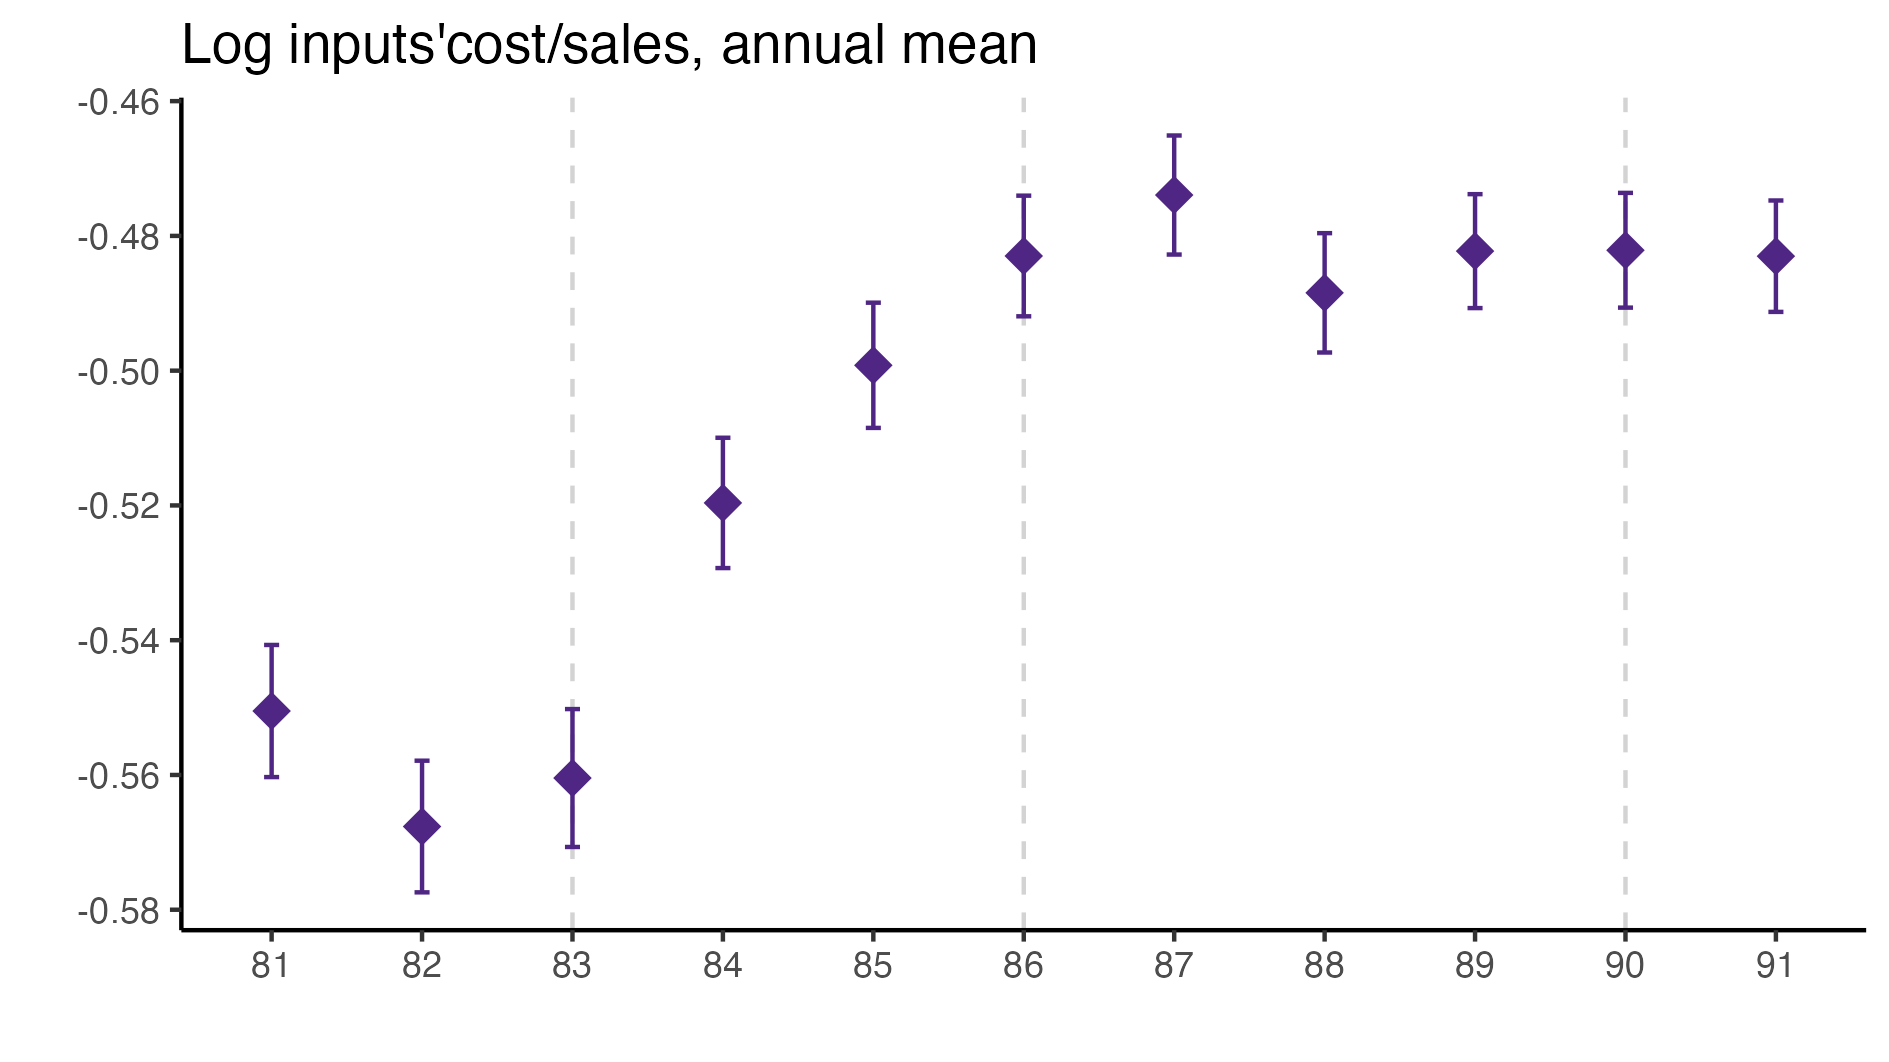
\includegraphics[width=1\textwidth,height=\textheight]{../Results/Figures/Colombia/log_share_byy.png}

}

\caption{\label{fig-logshare}Input's cost share of sales, average by
year of the logs.}

\end{figure}%

As a validation exercise, we can see that the VAT changes induced by the
three fiscal reforms are captured in the dataset. Figure~\ref{fig-vat}
shows that the sales tax increased to 10\% after the 1983 reform, and
then around 12\% after the 1990 reform.

\begin{figure}

\centering{

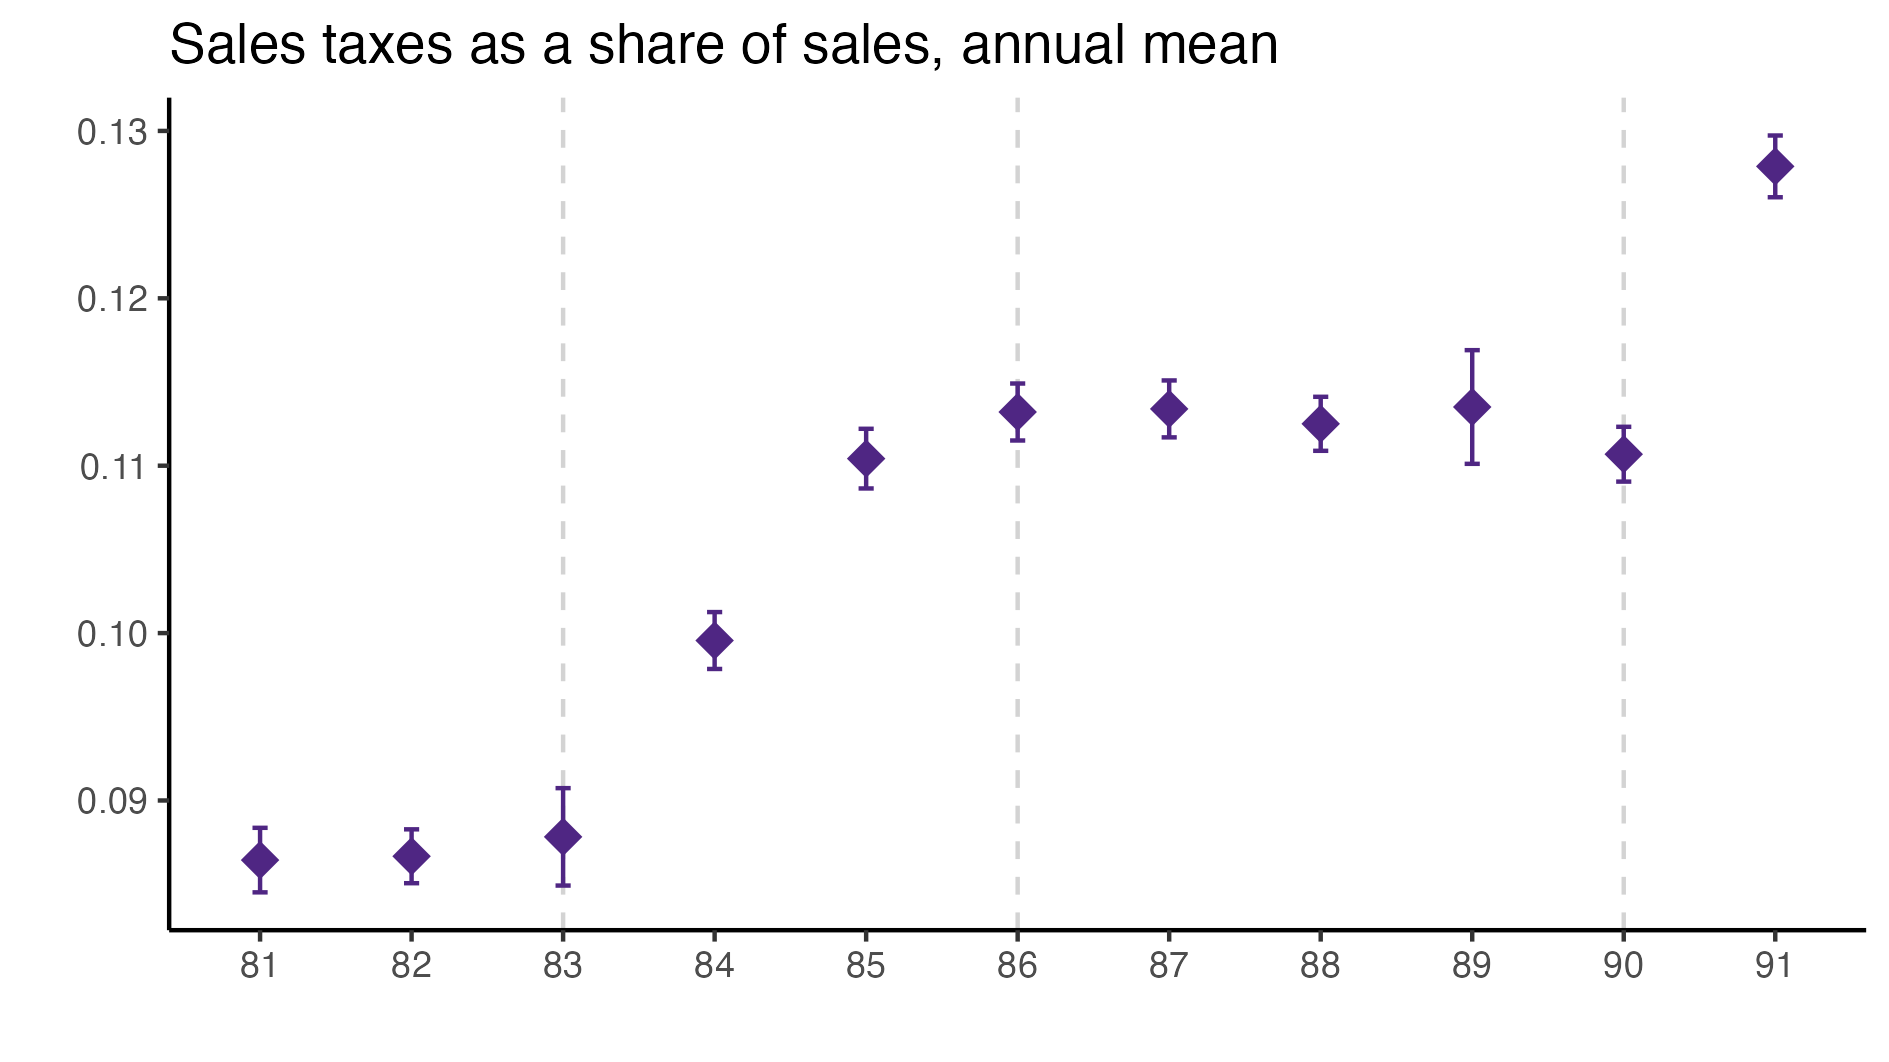
\includegraphics[width=1\textwidth,height=\textheight]{../Results/Figures/Colombia/share_sales_tax_byy.png}

}

\caption{\label{fig-vat}Sale taxes paid as share of sales, average by
year.}

\end{figure}%

Just as an exercise to see if other economic changes in this period were
driving the apparent changes in overreporting, Figure~\ref{fig-logsales}
shows that sales, for instance, were not exactly following the changes
in fiscal policy. Sales started to grow during 1983, the year of the
reform, whereas the cost share of sales started to grow the year after.
Likewise, sales fell in 1986, while the cost share seems to reduce its
growth after 1986.

\begin{figure}

\centering{

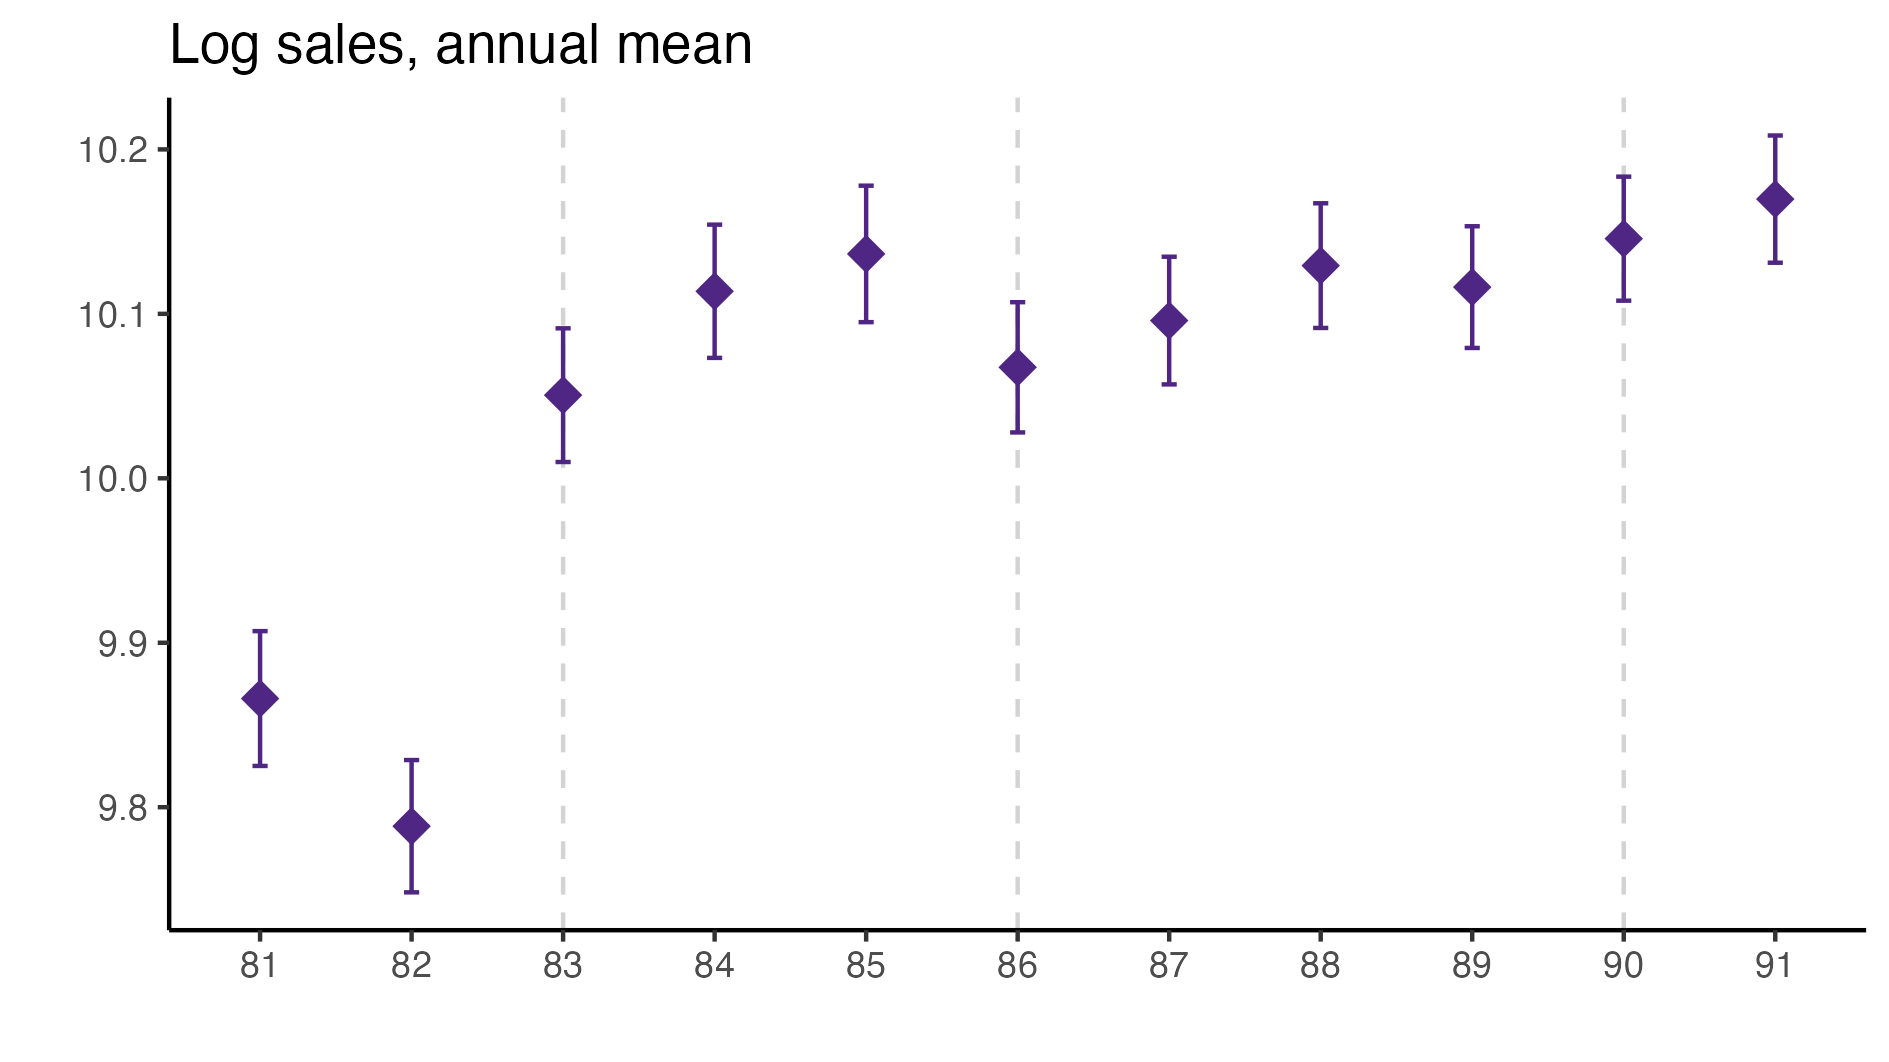
\includegraphics[width=1\textwidth,height=\textheight]{../Results/Figures/Colombia/log_sales_byy.png}

}

\caption{\label{fig-logsales}Sales in logs, annual mean.}

\end{figure}%

Finally, in a preliminary empirical assessment, I observe that the sales
tax rate is a significant determinant of the log share of revenue and
that non-corporations consistently use 13-17 percent more intermediates
than Corporations for a rich set of controls Table~\ref{tbl-reg-jo-tax}.
The results were estimated following Equation~\ref{eq-reg-tax-jo}

\begin{equation}\phantomsection\label{eq-reg-tax-jo}{
log(s_{it})= \alpha_1Tax_{it}+\beta_1'JurOrg_i + \beta_2'JurOrg_i\times\gamma_t+ \gamma_t + \gamma_{ind} +\gamma_{metro} + \beta_3'Z+ \varepsilon_{it}
}\end{equation}

\begin{table}

\caption{\label{tbl-reg-jo-tax}Effect of the Juridical Organization Type
and Sales Tax on the Log Share of Intermediate Inputs.}

\begin{minipage}{\linewidth}

\begingroup
\centering
\begin{tabular}{lccc}
   \tabularnewline \midrule \midrule
   Dependent Variable: & \multicolumn{3}{c}{Interm.}\\
   Model:         & (1)            & (2)            & (3)\\  
   \midrule
   \emph{Variables}\\
   Sales Tax Rate & 0.3898$^{**}$  & 0.4936$^{***}$ & 0.4597$^{***}$\\   
                  & (0.1334)       & (0.1283)       & (0.1302)\\   
   Proprietorship & 0.1626$^{***}$ & 0.1306$^{***}$ & 0.1279$^{***}$\\   
                  & (0.0243)       & (0.0178)       & (0.0170)\\   
   LLC            & 0.1720$^{***}$ & 0.1434$^{***}$ & 0.1386$^{***}$\\   
                  & (0.0259)       & (0.0191)       & (0.0189)\\   
   Partnership    & 0.1949$^{***}$ & 0.1666$^{***}$ & 0.1649$^{***}$\\   
                  & (0.0295)       & (0.0221)       & (0.0215)\\   
   \midrule
   \emph{Fixed-effects}\\
   Industry       &                & Yes            & Yes\\  
   Metro Area     &                &                & Yes\\  
   \midrule
   \emph{Fit statistics}\\
   Observations   & 41,830         & 41,830         & 41,830\\  
   R$^2$          & 0.56652        & 0.58206        & 0.58685\\  
   Within R$^2$   &                & 0.52466        & 0.52710\\  
   \midrule \midrule
   \multicolumn{4}{l}{\emph{Clustered (Industry \& Year) standard-errors in parentheses}}\\
   \multicolumn{4}{l}{\emph{Signif. Codes: ***: 0.01, **: 0.05, *: 0.1}}\\
\end{tabular}
\par\endgroup

\end{minipage}%

\end{table}%

Although this is not deterministic evidence, it does not contradict the
hypothesis that firms other than corporations have incentives to
overreport intermediates to evade taxes and that the higher the taxes
the higher the incentives to evade by misreporting.

\subsection{The Fiscal Reform of 1983 by
Industry}\label{the-fiscal-reform-of-1983-by-industry}

\begin{table}

\caption{\label{tbl-1983-by-inds}Fiscal reform of 1983. Sales tax share
of revenue, mean by industry year. Top 20 industries with more firms.}

\centering{

\centering
\begin{tblr}[         %% tabularray outer open
]                     %% tabularray outer close
{                     %% tabularray inner open
colspec={Q[]Q[]Q[]Q[]Q[]Q[]},
column{6}={halign=c,},
}                     %% tabularray inner close
\toprule
SIC & Industry & P&T (1990) & Change & Change Year & Annual Sales Tax (82-86) \\ \midrule %% TinyTableHeader
311 & Food Manufacturing &   & Exempt &  & 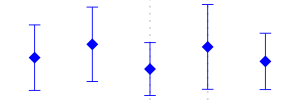
\includegraphics[height=4em]{tinytable_assets/idttwkr9hjm7rqx686gk7r.png} \\
312 & Food Manufacturing &   & Exempt &  & 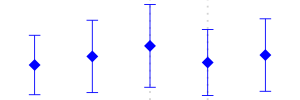
\includegraphics[height=4em]{tinytable_assets/idiyv41im4mg6nkm2wg4gt.png} \\
322 & Wearing Apparel, Except Footwear &   & Increased & 84 & 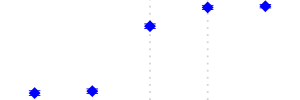
\includegraphics[height=4em]{tinytable_assets/id0izj0yivck85idl9894t.png} \\
381 & Fabricated Metal Products, Except Machinery and Equipment &   & Increased & 85 & 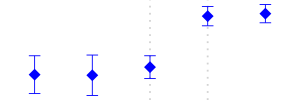
\includegraphics[height=4em]{tinytable_assets/idmb9bqvirpyl3g2fnqhsv.png} \\
321 & Textiles & 6 to 10 & Increased & 84 & 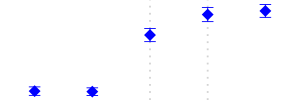
\includegraphics[height=4em]{tinytable_assets/idqrvsi9dg1rkakxbkl2ak.png} \\
382 & Machinery Except Electrical & 6 to 10 & Increased & 85 & 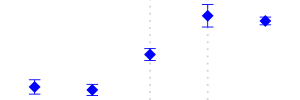
\includegraphics[height=4em]{tinytable_assets/id65qloayop02n5otw2kc2.png} \\
384 & Transport Equipment & 6 to 10 & Increased & 85 & 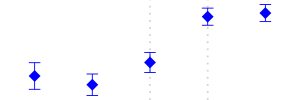
\includegraphics[height=4em]{tinytable_assets/id63m5wheliu93wgnkd6ia.png} \\
383 & Electrical Machinery Apparatus, Appliances and Supplies & 6 to 10 & Increased & 85 & 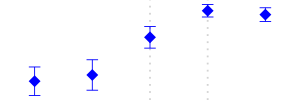
\includegraphics[height=4em]{tinytable_assets/idvtyb6gag43x9ashr5sw9.png} \\
313 & Beverage Industries & - to 35;10 & Increased & 85 & 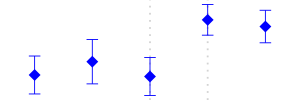
\includegraphics[height=4em]{tinytable_assets/id95qd82bfkig1u7s2ouw7.png} \\
341 & Paper and Paper Products & 15 to 10 & Increased & 84 & 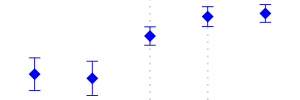
\includegraphics[height=4em]{tinytable_assets/idvxhezzfrlg694u4gppog.png} \\
324 & Footwear, Except Vulcanized or Moulded Rubber or Plastic Footwear &   & Increased & 84 & 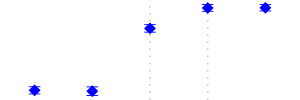
\includegraphics[height=4em]{tinytable_assets/idm2ag5i9o2erxypa0xsro.png} \\
342 & Printing, Publishing and Allied Industries &   & Decreased & 84 & 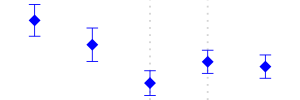
\includegraphics[height=4em]{tinytable_assets/idbdl71j3hcq5t8n2j2fxs.png} \\
369 & Other Non-Metallic Mineral Products &   & Decreased & 84 & 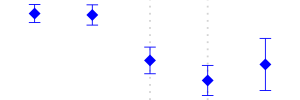
\includegraphics[height=4em]{tinytable_assets/idpd48np4fvzkrj9kq3trl.png} \\
390 & Other Manufacturing Industries &   & Decreased & 84 & 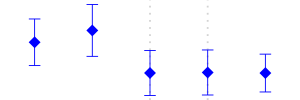
\includegraphics[height=4em]{tinytable_assets/id1zp3rcsgi53xyf3kcuy9.png} \\
332 & Furniture and Fixtures, Except Primarily of Metal &   & Decreased & 84 & 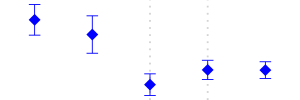
\includegraphics[height=4em]{tinytable_assets/id8pczr1flnu8yne8ok3xb.png} \\
351 & Industrial Chemicals & 15 to 10 & Decreased & 84 & 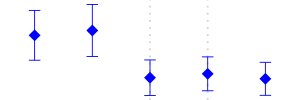
\includegraphics[height=4em]{tinytable_assets/idh8gqp4x0wnu8xvioljde.png} \\
352 & Other Chemical Products & 6;15 to 10 & No Change &  & 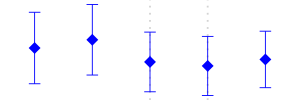
\includegraphics[height=4em]{tinytable_assets/id9dwht9hvtgli29fm8tej.png} \\
356 & Plastic Products Not Elsewhere Classified & 15 to 10 & No Change &  & 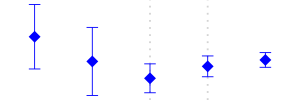
\includegraphics[height=4em]{tinytable_assets/idcc5hj2wlkutxf0b9rmqc.png} \\
331 & Wood and Wood and Cork Products, Except Furniture &   & No Change &  & 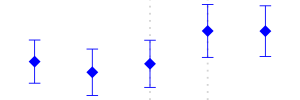
\includegraphics[height=4em]{tinytable_assets/idzsfrio7wx9fect1hws8u.png} \\
323 & Leather and Products of Leather, Leather Substitutes and Fur, Except Footwear and Wearing Apparel &   & No Change &  & 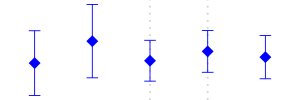
\includegraphics[height=4em]{tinytable_assets/id9ybj04uwfk06vij5ifap.png} \\
\bottomrule
\end{tblr}

}

\end{table}%

\section{Empirical Application}\label{empirical-application}

Given the fiscal reforms of 1983 and 1986 in Colombia, it is natural to
think in a difference-in-difference empirical application to test if the
fiscal reforms induced any change in the tax evasion behavior of the
firms. We can expect that an increase in either the sales tax or
corporate income tax rate would lead to higher levels of evasion.

Among other changes, the fiscal law of 1983 tried to homogenize the
sales taxes of the manufacturing industry. The reform reduced from 15 to
10\% for some industries; for others, it increased the sales tax from 6
to 10\%. Still, some others, like the Food Products industry were exempt
and certain others were not affected. See Table~\ref{tbl-vat-summary}
for a description of the changes documented in \citet{Perry1990}.

The 1983 reform also adjusted the income tax rates for limited liability
companies and individuals. For individuals, the income tax rate
increased by 8\% in most scales, while the maximum was reduced from 56
to 49\%. For limited liability companies, the CIT was reduced from 10 to
18\%.

To evaluate the change in tax evasion by input cost overreporting due to
the change in the sales tax, I apply a triple difference approach. I use
corporations in the industries exempted from sales taxes the year before
the policy change as the control group.

Formally, non-corporations in industry \(k\), which might have received
an increment or decrement in their sales tax rate,

\[
s_{1,j,t}^k=\lambda^k_t+\mu^k_1+e^{VAT}_{j,t}+e^{CIT}_{j,t}+\varepsilon_{jt}
\]

Corporations in industry \(k\), \[
s_{0,j,t}^k=\lambda^k_t+\mu^k_0+\varepsilon_{jt}
\]

Likewise, Non-corporations and Corporations in an industry exempt from
sales taxes

\[
\begin{aligned}
    s_{1,j,t}^{E}&=\lambda^{E}_t+\mu^E_1+e^{CIT}_{j,t}+\varepsilon_{jt}\\
    s_{0,j,t}^E&=\lambda^E_t+\mu^E_0+\varepsilon_{jt}
\end{aligned}
\]

Taking the difference between time \(t'\) and \(t\) in industry \(k\)
for both, corporations and non-corporations,

\[
\begin{aligned}
    \mathbb{E}[s_{1,j,t'}^k]-\mathbb{E}[s_{1,j,t}^k]&=\Delta_\lambda^k+\Delta_e^{VAT}+\Delta_e^{CIT}\\
    \mathbb{E}[s_{0,j,t'}^k]-\mathbb{E}[s_{0,j,t}^k]&=\Delta_\lambda^k
\end{aligned}
\]

The diff-in-diff method will recover the joint effect of both policy
changes, \[
\mathbb{E}[s_{1,j,t'}^k]-\mathbb{E}[s_{1,j,t}^k]-\left(\mathbb{E}[s_{0,j,t'}^k]-\mathbb{E}[s_{0,j,t}^k]\right)=\Delta_e^{VAT}+\Delta_e^{CIT}
\]

The joint effect might be ambiguous because an increase in the sales tax
rate will increase the incentive to overreport inputs cost but a
decrease in the CIT might decrease the incentive.

To recover the effect of the change in the sales tax rate, we can use
the firms of the industries that are exempted from the sales tax.
Intuitively, exempted firms would not react to the change in the sales
tax ---which is industry-specific---, but only to the CIT ---which
affects all industries.

So we have,

\[
\begin{aligned}    
    \mathbb{E}[s_{1,j,t'}^k]&-\mathbb{E}[s_{1,j,t}^k]-\left(\mathbb{E}[s_{0,j,t'}^k]-\mathbb{E}[s_{0,j,t}^k]\right)\\ 
    &- \left[\mathbb{E}[s_{1,j,t'}^{E}]-\mathbb{E}[s_{1,j,t}^{E}]-\left(\mathbb{E}[s_{0,j,t'}^{E}]-\mathbb{E}[s_{0,j,t}^{E}]\right)\right]=\Delta_e^{VAT}
\end{aligned}
\]

In regression form,

\[
s_{jt}=\alpha \left[ \mathbb{1}\{t=t'\}\times\mathbb{1}\{\text{treat}=\text{Non-Corp}\}\times\mathbb{1}\{k\not=E\} \right]+\beta'_ZZ_{jt}+\gamma_j+\gamma_t+\varepsilon_{jt}
\]

\begin{table}

\caption{\label{tbl-reg-didid}Log of Inputs Cost Share of Revenue by
Industry. Triple diff-in-diff. The reference group is Corporations in
industries exempted from the Tax Rate the year before the Reform of 1983
(1982).}

\begin{minipage}{\linewidth}

\begingroup
\centering
\begin{tabular}{lcccc}
   \tabularnewline \midrule \midrule
   Dependent Variables:                                    & log\_mats\_share   & log\_energy\_share   & log\_fuels\_share   & log\_repair\_maint\_share\\     
   Industry & \multicolumn{4}{c}{Wearing Apparel, Except Footwe...} \\ 
   Tax Change & \multicolumn{4}{c}{Increased} \\ 
   Model:                                                  & (1)                & (2)                  & (3)                 & (4)\\  
   \midrule
   \emph{Variables}\\
   1984 $\times$ Non-Corp. $\times$ treat\_3tax\_treat     & 0.0842$^{**}$      & -0.0708              & -0.0235             & 0.0130\\   
                                                           & (0.0315)           & (0.0496)             & (0.0571)            & (0.0754)\\   
   1985 $\times$ Non-Corp. $\times$ treat\_3tax\_treat     & 0.3449$^{***}$     & 0.0248               & 0.2256$^{**}$       & 0.0416\\   
                                                           & (0.0628)           & (0.0621)             & (0.0871)            & (0.0966)\\   
   1986 $\times$ Non-Corp. $\times$ treat\_3tax\_treat     & 0.1842$^{***}$     & 0.0385               & 0.1604$^{*}$        & -0.1082\\   
                                                           & (0.0495)           & (0.0733)             & (0.0802)            & (0.0957)\\   
   \midrule
   \emph{Fixed-effects}\\
   plant                                                   & Yes                & Yes                  & Yes                 & Yes\\  
   Year                                                    & Yes                & Yes                  & Yes                 & Yes\\  
   \midrule
   \emph{Fit statistics}\\
   Observations                                            & 10,399             & 10,410               & 9,320               & 9,069\\  
   R$^2$                                                   & 0.77685            & 0.85498              & 0.83131             & 0.61253\\  
   Within R$^2$                                            & 0.01625            & 0.01232              & 0.01154             & 0.00610\\  
   \midrule \midrule
   \multicolumn{5}{l}{\emph{Clustered (Year) standard-errors in parentheses}}\\
   \multicolumn{5}{l}{\emph{Signif. Codes: ***: 0.01, **: 0.05, *: 0.1}}\\
\end{tabular}
\par\endgroup
\begingroup
\centering
\begin{tabular}{lcccc}
   \tabularnewline \midrule \midrule
   Dependent Variables:                                    & log\_mats\_share   & log\_energy\_share   & log\_fuels\_share   & log\_repair\_maint\_share\\     
   Industry & \multicolumn{4}{c}{Fabricated Metal Products, Exc...} \\ 
   Tax Change & \multicolumn{4}{c}{Increased} \\ 
   Model:                                                  & (1)                & (2)                  & (3)                 & (4)\\  
   \midrule
   \emph{Variables}\\
   1984 $\times$ Non-Corp. $\times$ treat\_3tax\_treat     & 0.0365$^{*}$       & 0.0836               & 0.0492$^{*}$        & -0.0882\\   
                                                           & (0.0172)           & (0.0529)             & (0.0264)            & (0.0657)\\   
   1985 $\times$ Non-Corp. $\times$ treat\_3tax\_treat     & 0.2405$^{***}$     & 0.1020$^{***}$       & 0.1184$^{***}$      & 0.3603$^{***}$\\   
                                                           & (0.0339)           & (0.0247)             & (0.0355)            & (0.0702)\\   
   1986 $\times$ Non-Corp. $\times$ treat\_3tax\_treat     & 0.0379             & 0.0538               & 0.0660$^{*}$        & 0.2295$^{***}$\\   
                                                           & (0.0256)           & (0.0519)             & (0.0331)            & (0.0711)\\   
   \midrule
   \emph{Fixed-effects}\\
   plant                                                   & Yes                & Yes                  & Yes                 & Yes\\  
   Year                                                    & Yes                & Yes                  & Yes                 & Yes\\  
   \midrule
   \emph{Fit statistics}\\
   Observations                                            & 9,687              & 9,665                & 9,126               & 8,304\\  
   R$^2$                                                   & 0.73677            & 0.85826              & 0.78781             & 0.59819\\  
   Within R$^2$                                            & 0.00880            & 0.01441              & 0.00850             & 0.00999\\  
   \midrule \midrule
   \multicolumn{5}{l}{\emph{Clustered (Year) standard-errors in parentheses}}\\
   \multicolumn{5}{l}{\emph{Signif. Codes: ***: 0.01, **: 0.05, *: 0.1}}\\
\end{tabular}
\par\endgroup
\begingroup
\centering
\begin{tabular}{lcccc}
   \tabularnewline \midrule \midrule
   Dependent Variables:                                    & log\_mats\_share   & log\_energy\_share   & log\_fuels\_share   & log\_repair\_maint\_share\\     
   Industry & \multicolumn{4}{c}{Textiles...} \\ 
   Tax Change & \multicolumn{4}{c}{Increased} \\ 
   Model:                                                  & (1)                & (2)                  & (3)                 & (4)\\  
   \midrule
   \emph{Variables}\\
   1984 $\times$ Non-Corp. $\times$ treat\_3tax\_treat     & -0.0220            & 0.0899$^{***}$       & -0.0840$^{*}$       & -0.0682\\   
                                                           & (0.0246)           & (0.0110)             & (0.0423)            & (0.0430)\\   
   1985 $\times$ Non-Corp. $\times$ treat\_3tax\_treat     & 0.0114             & 0.2372$^{***}$       & 0.3169$^{***}$      & 0.1221$^{***}$\\   
                                                           & (0.0263)           & (0.0213)             & (0.0606)            & (0.0286)\\   
   1986 $\times$ Non-Corp. $\times$ treat\_3tax\_treat     & 0.0532             & 0.2808$^{***}$       & 0.2053$^{**}$       & 0.1147$^{**}$\\   
                                                           & (0.0352)           & (0.0287)             & (0.0656)            & (0.0414)\\   
   \midrule
   \emph{Fixed-effects}\\
   plant                                                   & Yes                & Yes                  & Yes                 & Yes\\  
   Year                                                    & Yes                & Yes                  & Yes                 & Yes\\  
   \midrule
   \emph{Fit statistics}\\
   Observations                                            & 8,777              & 8,751                & 8,298               & 7,704\\  
   R$^2$                                                   & 0.74339            & 0.86051              & 0.81090             & 0.60366\\  
   Within R$^2$                                            & 0.00745            & 0.01116              & 0.01961             & 0.00974\\  
   \midrule \midrule
   \multicolumn{5}{l}{\emph{Clustered (Year) standard-errors in parentheses}}\\
   \multicolumn{5}{l}{\emph{Signif. Codes: ***: 0.01, **: 0.05, *: 0.1}}\\
\end{tabular}
\par\endgroup
\begingroup
\centering
\begin{tabular}{lcccc}
   \tabularnewline \midrule \midrule
   Dependent Variables:                                    & log\_mats\_share   & log\_energy\_share   & log\_fuels\_share   & log\_repair\_maint\_share\\     
   Industry & \multicolumn{4}{c}{Other Chemical Products...} \\ 
   Tax Change & \multicolumn{4}{c}{No Change} \\ 
   Model:                                                  & (1)                & (2)                  & (3)                 & (4)\\  
   \midrule
   \emph{Variables}\\
   1984 $\times$ Non-Corp. $\times$ treat\_3tax\_treat     & 0.0656             & 0.0769$^{***}$       & -0.3550$^{***}$     & -0.1721$^{***}$\\   
                                                           & (0.0443)           & (0.0120)             & (0.0406)            & (0.0473)\\   
   1985 $\times$ Non-Corp. $\times$ treat\_3tax\_treat     & 0.1058$^{*}$       & 0.2417$^{***}$       & 0.0808              & 0.0690$^{*}$\\   
                                                           & (0.0541)           & (0.0132)             & (0.0535)            & (0.0357)\\   
   1986 $\times$ Non-Corp. $\times$ treat\_3tax\_treat     & 0.0358             & 0.1365$^{***}$       & 0.1978$^{***}$      & 0.3642$^{***}$\\   
                                                           & (0.0467)           & (0.0293)             & (0.0621)            & (0.0449)\\   
   \midrule
   \emph{Fixed-effects}\\
   plant                                                   & Yes                & Yes                  & Yes                 & Yes\\  
   Year                                                    & Yes                & Yes                  & Yes                 & Yes\\  
   \midrule
   \emph{Fit statistics}\\
   Observations                                            & 8,232              & 8,229                & 7,683               & 7,327\\  
   R$^2$                                                   & 0.75077            & 0.87588              & 0.81684             & 0.60844\\  
   Within R$^2$                                            & 0.00673            & 0.01677              & 0.01136             & 0.00932\\  
   \midrule \midrule
   \multicolumn{5}{l}{\emph{Clustered (Year) standard-errors in parentheses}}\\
   \multicolumn{5}{l}{\emph{Signif. Codes: ***: 0.01, **: 0.05, *: 0.1}}\\
\end{tabular}
\par\endgroup
\begingroup
\centering
\begin{tabular}{lcccc}
   \tabularnewline \midrule \midrule
   Dependent Variables:                                    & log\_mats\_share   & log\_energy\_share   & log\_fuels\_share   & log\_repair\_maint\_share\\     
   Industry & \multicolumn{4}{c}{Machinery Except Electrical...} \\ 
   Tax Change & \multicolumn{4}{c}{Increased} \\ 
   Model:                                                  & (1)                & (2)                  & (3)                 & (4)\\  
   \midrule
   \emph{Variables}\\
   1984 $\times$ Non-Corp. $\times$ treat\_3tax\_treat     & 0.0101             & -0.0281              & -0.4425$^{***}$     & -0.2643$^{***}$\\   
                                                           & (0.0095)           & (0.0372)             & (0.0560)            & (0.0787)\\   
   1985 $\times$ Non-Corp. $\times$ treat\_3tax\_treat     & 0.1142$^{***}$     & -0.0040              & -0.4888$^{***}$     & -0.3648$^{***}$\\   
                                                           & (0.0328)           & (0.0439)             & (0.0781)            & (0.0819)\\   
   1986 $\times$ Non-Corp. $\times$ treat\_3tax\_treat     & 0.0002             & 0.0835               & -0.2281$^{*}$       & -0.3348$^{***}$\\   
                                                           & (0.0286)           & (0.0555)             & (0.1151)            & (0.0665)\\   
   \midrule
   \emph{Fixed-effects}\\
   plant                                                   & Yes                & Yes                  & Yes                 & Yes\\  
   Year                                                    & Yes                & Yes                  & Yes                 & Yes\\  
   \midrule
   \emph{Fit statistics}\\
   Observations                                            & 8,162              & 8,159                & 7,757               & 7,097\\  
   R$^2$                                                   & 0.75493            & 0.86454              & 0.80169             & 0.61290\\  
   Within R$^2$                                            & 0.00914            & 0.01112              & 0.00827             & 0.01111\\  
   \midrule \midrule
   \multicolumn{5}{l}{\emph{Clustered (Year) standard-errors in parentheses}}\\
   \multicolumn{5}{l}{\emph{Signif. Codes: ***: 0.01, **: 0.05, *: 0.1}}\\
\end{tabular}
\par\endgroup
\begingroup
\centering
\begin{tabular}{lcccc}
   \tabularnewline \midrule \midrule
   Dependent Variables:                                    & log\_mats\_share   & log\_energy\_share   & log\_fuels\_share   & log\_repair\_maint\_share\\     
   Industry & \multicolumn{4}{c}{Printing, Publishing and Allie...} \\ 
   Tax Change & \multicolumn{4}{c}{Decreased} \\ 
   Model:                                                  & (1)                & (2)                  & (3)                 & (4)\\  
   \midrule
   \emph{Variables}\\
   1984 $\times$ Non-Corp. $\times$ treat\_3tax\_treat     & -0.0175            & 0.0755$^{***}$       & -0.2410$^{***}$     & 0.2644$^{**}$\\   
                                                           & (0.0177)           & (0.0193)             & (0.0423)            & (0.0994)\\   
   1985 $\times$ Non-Corp. $\times$ treat\_3tax\_treat     & 0.1218$^{***}$     & 0.2200$^{***}$       & 0.1060              & 0.3960$^{***}$\\   
                                                           & (0.0381)           & (0.0214)             & (0.0734)            & (0.0640)\\   
   1986 $\times$ Non-Corp. $\times$ treat\_3tax\_treat     & 0.0509             & 0.2090$^{***}$       & 0.0624              & 0.1649\\   
                                                           & (0.0390)           & (0.0407)             & (0.0836)            & (0.1020)\\   
   \midrule
   \emph{Fixed-effects}\\
   plant                                                   & Yes                & Yes                  & Yes                 & Yes\\  
   Year                                                    & Yes                & Yes                  & Yes                 & Yes\\  
   \midrule
   \emph{Fit statistics}\\
   Observations                                            & 8,011              & 7,995                & 7,581               & 7,202\\  
   R$^2$                                                   & 0.75331            & 0.86250              & 0.81356             & 0.62650\\  
   Within R$^2$                                            & 0.00755            & 0.01452              & 0.01240             & 0.01063\\  
   \midrule \midrule
   \multicolumn{5}{l}{\emph{Clustered (Year) standard-errors in parentheses}}\\
   \multicolumn{5}{l}{\emph{Signif. Codes: ***: 0.01, **: 0.05, *: 0.1}}\\
\end{tabular}
\par\endgroup
\begingroup
\centering
\begin{tabular}{lcccc}
   \tabularnewline \midrule \midrule
   Dependent Variables:                                    & log\_mats\_share   & log\_energy\_share   & log\_fuels\_share   & log\_repair\_maint\_share\\     
   Industry & \multicolumn{4}{c}{Other Non-Metallic Mineral Pro...} \\ 
   Tax Change & \multicolumn{4}{c}{Decreased} \\ 
   Model:                                                  & (1)                & (2)                  & (3)                 & (4)\\  
   \midrule
   \emph{Variables}\\
   1984 $\times$ Non-Corp. $\times$ treat\_3tax\_treat     & 0.1175$^{*}$       & -0.0031              & -0.0256             & 0.2628$^{***}$\\   
                                                           & (0.0536)           & (0.0210)             & (0.0426)            & (0.0495)\\   
   1985 $\times$ Non-Corp. $\times$ treat\_3tax\_treat     & -0.0790            & 0.1781$^{***}$       & 0.2629$^{***}$      & 0.1275$^{**}$\\   
                                                           & (0.0556)           & (0.0305)             & (0.0367)            & (0.0409)\\   
   1986 $\times$ Non-Corp. $\times$ treat\_3tax\_treat     & 0.1110             & 0.1261$^{***}$       & 0.3077$^{***}$      & -0.0063\\   
                                                           & (0.0917)           & (0.0289)             & (0.0395)            & (0.0563)\\   
   \midrule
   \emph{Fixed-effects}\\
   plant                                                   & Yes                & Yes                  & Yes                 & Yes\\  
   Year                                                    & Yes                & Yes                  & Yes                 & Yes\\  
   \midrule
   \emph{Fit statistics}\\
   Observations                                            & 7,855              & 7,899                & 7,608               & 7,053\\  
   R$^2$                                                   & 0.78671            & 0.88390              & 0.84337             & 0.66387\\  
   Within R$^2$                                            & 0.01981            & 0.01099              & 0.01145             & 0.01233\\  
   \midrule \midrule
   \multicolumn{5}{l}{\emph{Clustered (Year) standard-errors in parentheses}}\\
   \multicolumn{5}{l}{\emph{Signif. Codes: ***: 0.01, **: 0.05, *: 0.1}}\\
\end{tabular}
\par\endgroup
\begingroup
\centering
\begin{tabular}{lcccc}
   \tabularnewline \midrule \midrule
   Dependent Variables:                                    & log\_mats\_share   & log\_energy\_share   & log\_fuels\_share   & log\_repair\_maint\_share\\     
   Industry & \multicolumn{4}{c}{Plastic Products Not Elsewhere...} \\ 
   Tax Change & \multicolumn{4}{c}{No Change} \\ 
   Model:                                                  & (1)                & (2)                  & (3)                 & (4)\\  
   \midrule
   \emph{Variables}\\
   1984 $\times$ Non-Corp. $\times$ treat\_3tax\_treat     & 0.0902$^{***}$     & 0.0050               & -0.2032$^{***}$     & 0.5201$^{***}$\\   
                                                           & (0.0165)           & (0.0227)             & (0.0558)            & (0.0977)\\   
   1985 $\times$ Non-Corp. $\times$ treat\_3tax\_treat     & 0.1940$^{***}$     & 0.0442               & -0.0272             & 0.3438$^{***}$\\   
                                                           & (0.0426)           & (0.0323)             & (0.0881)            & (0.0527)\\   
   1986 $\times$ Non-Corp. $\times$ treat\_3tax\_treat     & 0.1195$^{***}$     & 0.1372$^{***}$       & 0.2778$^{***}$      & -0.0255\\   
                                                           & (0.0300)           & (0.0387)             & (0.0743)            & (0.0803)\\   
   \midrule
   \emph{Fixed-effects}\\
   plant                                                   & Yes                & Yes                  & Yes                 & Yes\\  
   Year                                                    & Yes                & Yes                  & Yes                 & Yes\\  
   \midrule
   \emph{Fit statistics}\\
   Observations                                            & 7,640              & 7,641                & 7,246               & 6,685\\  
   R$^2$                                                   & 0.74766            & 0.86716              & 0.82520             & 0.61785\\  
   Within R$^2$                                            & 0.00493            & 0.00891              & 0.01282             & 0.00817\\  
   \midrule \midrule
   \multicolumn{5}{l}{\emph{Clustered (Year) standard-errors in parentheses}}\\
   \multicolumn{5}{l}{\emph{Signif. Codes: ***: 0.01, **: 0.05, *: 0.1}}\\
\end{tabular}
\par\endgroup
\begingroup
\centering
\begin{tabular}{lcccc}
   \tabularnewline \midrule \midrule
   Dependent Variables:                                    & log\_mats\_share   & log\_energy\_share   & log\_fuels\_share   & log\_repair\_maint\_share\\     
   Industry & \multicolumn{4}{c}{Transport Equipment...} \\ 
   Tax Change & \multicolumn{4}{c}{Increased} \\ 
   Model:                                                  & (1)                & (2)                  & (3)                 & (4)\\  
   \midrule
   \emph{Variables}\\
   1984 $\times$ Non-Corp. $\times$ treat\_3tax\_treat     & 0.1127$^{***}$     & -0.0499$^{**}$       & -0.1458$^{**}$      & 0.0081\\   
                                                           & (0.0120)           & (0.0194)             & (0.0509)            & (0.0486)\\   
   1985 $\times$ Non-Corp. $\times$ treat\_3tax\_treat     & 0.0477             & -0.0041              & 0.1727$^{***}$      & 0.4006$^{***}$\\   
                                                           & (0.0351)           & (0.0145)             & (0.0294)            & (0.0774)\\   
   1986 $\times$ Non-Corp. $\times$ treat\_3tax\_treat     & -0.0323            & -0.0749$^{**}$       & 0.0406              & 0.2173$^{**}$\\   
                                                           & (0.0263)           & (0.0311)             & (0.0602)            & (0.0746)\\   
   \midrule
   \emph{Fixed-effects}\\
   plant                                                   & Yes                & Yes                  & Yes                 & Yes\\  
   Year                                                    & Yes                & Yes                  & Yes                 & Yes\\  
   \midrule
   \emph{Fit statistics}\\
   Observations                                            & 7,442              & 7,439                & 7,101               & 6,543\\  
   R$^2$                                                   & 0.74608            & 0.86173              & 0.81971             & 0.62395\\  
   Within R$^2$                                            & 0.00853            & 0.01940              & 0.01192             & 0.01368\\  
   \midrule \midrule
   \multicolumn{5}{l}{\emph{Clustered (Year) standard-errors in parentheses}}\\
   \multicolumn{5}{l}{\emph{Signif. Codes: ***: 0.01, **: 0.05, *: 0.1}}\\
\end{tabular}
\par\endgroup
\begingroup
\centering
\begin{tabular}{lcccc}
   \tabularnewline \midrule \midrule
   Dependent Variables:                                    & log\_mats\_share   & log\_energy\_share   & log\_fuels\_share   & log\_repair\_maint\_share\\     
   Industry & \multicolumn{4}{c}{Electrical Machinery Apparatus...} \\ 
   Tax Change & \multicolumn{4}{c}{Increased} \\ 
   Model:                                                  & (1)                & (2)                  & (3)                 & (4)\\  
   \midrule
   \emph{Variables}\\
   1984 $\times$ Non-Corp. $\times$ treat\_3tax\_treat     & 0.0541$^{***}$     & 0.0296               & -0.0559             & -0.0221\\   
                                                           & (0.0107)           & (0.0219)             & (0.0412)            & (0.0709)\\   
   1985 $\times$ Non-Corp. $\times$ treat\_3tax\_treat     & 0.1140$^{***}$     & 0.1462$^{***}$       & 0.2673$^{***}$      & 0.3297$^{***}$\\   
                                                           & (0.0263)           & (0.0321)             & (0.0586)            & (0.0845)\\   
   1986 $\times$ Non-Corp. $\times$ treat\_3tax\_treat     & 0.1197$^{***}$     & 0.0433               & 0.3565$^{***}$      & 0.3712$^{***}$\\   
                                                           & (0.0212)           & (0.0320)             & (0.0596)            & (0.0633)\\   
   \midrule
   \emph{Fixed-effects}\\
   plant                                                   & Yes                & Yes                  & Yes                 & Yes\\  
   Year                                                    & Yes                & Yes                  & Yes                 & Yes\\  
   \midrule
   \emph{Fit statistics}\\
   Observations                                            & 7,400              & 7,398                & 6,995               & 6,532\\  
   R$^2$                                                   & 0.74902            & 0.85999              & 0.81695             & 0.60898\\  
   Within R$^2$                                            & 0.00479            & 0.01269              & 0.00640             & 0.01019\\  
   \midrule \midrule
   \multicolumn{5}{l}{\emph{Clustered (Year) standard-errors in parentheses}}\\
   \multicolumn{5}{l}{\emph{Signif. Codes: ***: 0.01, **: 0.05, *: 0.1}}\\
\end{tabular}
\par\endgroup

\end{minipage}%

\end{table}%

\subsection{Changes in Composition of Total
Expenditure}\label{changes-in-composition-of-total-expenditure}

Depending on the industry, firms might be adjusting different margins,
raw materials or other expenses. For example, firms in the non-metallic
mineral products industry might not fake raw materials but they can
adjust deductible expenses. Another example might be the textile
industry. Although the available records and data might not allow for
separating expenditures precisely, the evidence shows that firms are
significantly adjusting these margins.

\citet{Gandhi2020} defines services as general expenditures minus
machinery rental and interest payments. The Colombian survey uses
industrial expenditure to calculate intermediate consumption. I
identified potentially deductible expenses with information from
\citet{Perry1990}.

\begin{table}

\caption{\label{tbl-expenses-type}Classifications of Expenditure.}

\centering{

\centering
\begin{tabular}[t]{l|c|c|c|c}
\hline
Expenditure & Code & Services & Industrial & Deductible\\
\hline
Purchases of accessories and replacement parts of less than one year duration & c1 &  & \$+\$ & \\
\hline
Purchases of fuels and lubricants consumed by the establishment & c2 &  & \$+\$ & \$+\$\\
\hline
Payments for industrial work by other establishments & c3 &  & \$+\$ & \\
\hline
Payment of domestic workers & c4 &  & \$+\$ & \\
\hline
Payments of third parties for repairs and maintenance & c5 &  & \$+\$ & \$+\$\\
\hline
Purchases of raw materials and goods sold without transformation & c6 &  & \$+\$ & \$+\$\\
\hline
\textbf{TOTAL Industrial Expenditures (c1:c6)} & \textbf{c7} & \textbf{} & \textbf{} & \textbf{}\\
\hline
\hline
Rent of fixed property & c8 & \$+\$ &  & \\
\hline
Payments for professional services & c9 & \$+\$ &  & \\
\hline
Machinery rental & c10 &  &  & \$+\$\\
\hline
Insurance, excl. employe benefits & c11 & \$+\$ &  & \$+\$\\
\hline
Water, mail, telephone, etc. & c12 & \$+\$ &  & \$+\$\\
\hline
Publicity and advertising & c13 & \$+\$ &  & \\
\hline
Interest payments & c14 &  &  & \\
\hline
Royalty payments & c15 & \$+\$ &  & \\
\hline
Other expenditures & c16 & \$+\$ &  & \\
\hline
\textbf{TOTAL General Expenditures (c8:c16)} & \textbf{c17} & \textbf{} & \textbf{} & \textbf{}\\
\hline
\hline
\textbf{TOTAL Expenditure (c7+c17)} & \textbf{} & \textbf{} & \textbf{} & \textbf{}\\
\hline
\hline
\end{tabular}

}

\end{table}%

\begin{table}

\caption{\label{tbl-reg-exp-inds}Log of Types of Expenses Share of Total
Expenses by Industry. Triple diff-in-diff. The reference group is
Corporations in industries exempted from the Tax Rate the year before
the Reform of 1983 (1982).}

\begin{minipage}{\linewidth}

\begingroup
\centering
\begin{tabular}{lcc}
   \tabularnewline \midrule \midrule
   Dependent Variables:                                    & log\_services\_share   & log\_inds\_nded\_share\\     
   Industry & \multicolumn{2}{c}{322–Wearing Apparel, Except Fo...} \\ 
   Tax Change & \multicolumn{2}{c}{Increased} \\ 
   Model:                                                  & (1)                    & (2)\\  
   \midrule
   \emph{Variables}\\
   1984 $\times$ Non-Corp. $\times$ treat\_3tax\_treat     & -0.1164$^{**}$         & -0.7212$^{***}$\\   
                                                           & (0.0469)               & (0.0901)\\   
   1985 $\times$ Non-Corp. $\times$ treat\_3tax\_treat     & 0.0751                 & -0.3606$^{***}$\\   
                                                           & (0.0560)               & (0.0900)\\   
   1986 $\times$ Non-Corp. $\times$ treat\_3tax\_treat     & 0.0201                 & -0.4297$^{***}$\\   
                                                           & (0.0503)               & (0.0946)\\   
   \midrule
   \emph{Fixed-effects}\\
   plant                                                   & Yes                    & Yes\\  
   Year                                                    & Yes                    & Yes\\  
   \midrule
   \emph{Fit statistics}\\
   Observations                                            & 10,508                 & 10,120\\  
   R$^2$                                                   & 0.72910                & 0.65397\\  
   Within R$^2$                                            & 0.01639                & 0.01278\\  
   \midrule \midrule
   \multicolumn{3}{l}{\emph{Clustered (Year) standard-errors in parentheses}}\\
   \multicolumn{3}{l}{\emph{Signif. Codes: ***: 0.01, **: 0.05, *: 0.1}}\\
\end{tabular}
\par\endgroup
\begingroup
\centering
\begin{tabular}{lcc}
   \tabularnewline \midrule \midrule
   Dependent Variables:                                    & log\_services\_share   & log\_inds\_nded\_share\\     
   Industry & \multicolumn{2}{c}{381–Fabricated Metal Products,...} \\ 
   Tax Change & \multicolumn{2}{c}{Increased} \\ 
   Model:                                                  & (1)                    & (2)\\  
   \midrule
   \emph{Variables}\\
   1984 $\times$ Non-Corp. $\times$ treat\_3tax\_treat     & 0.0434$^{**}$          & -0.3378$^{***}$\\   
                                                           & (0.0166)               & (0.0453)\\   
   1985 $\times$ Non-Corp. $\times$ treat\_3tax\_treat     & 0.1703$^{***}$         & -0.2469$^{***}$\\   
                                                           & (0.0275)               & (0.0653)\\   
   1986 $\times$ Non-Corp. $\times$ treat\_3tax\_treat     & 0.0412                 & -0.2238$^{***}$\\   
                                                           & (0.0285)               & (0.0639)\\   
   \midrule
   \emph{Fixed-effects}\\
   plant                                                   & Yes                    & Yes\\  
   Year                                                    & Yes                    & Yes\\  
   \midrule
   \emph{Fit statistics}\\
   Observations                                            & 9,741                  & 9,340\\  
   R$^2$                                                   & 0.74553                & 0.68307\\  
   Within R$^2$                                            & 0.01784                & 0.00741\\  
   \midrule \midrule
   \multicolumn{3}{l}{\emph{Clustered (Year) standard-errors in parentheses}}\\
   \multicolumn{3}{l}{\emph{Signif. Codes: ***: 0.01, **: 0.05, *: 0.1}}\\
\end{tabular}
\par\endgroup
\begingroup
\centering
\begin{tabular}{lcc}
   \tabularnewline \midrule \midrule
   Dependent Variables:                                    & log\_services\_share   & log\_inds\_nded\_share\\     
   Industry & \multicolumn{2}{c}{321–Textiles...} \\ 
   Tax Change & \multicolumn{2}{c}{Increased} \\ 
   Model:                                                  & (1)                    & (2)\\  
   \midrule
   \emph{Variables}\\
   1984 $\times$ Non-Corp. $\times$ treat\_3tax\_treat     & -0.0914$^{***}$        & -0.2771$^{***}$\\   
                                                           & (0.0171)               & (0.0205)\\   
   1985 $\times$ Non-Corp. $\times$ treat\_3tax\_treat     & 0.0668$^{*}$           & -0.5449$^{***}$\\   
                                                           & (0.0312)               & (0.0218)\\   
   1986 $\times$ Non-Corp. $\times$ treat\_3tax\_treat     & 0.0588$^{*}$           & -0.5935$^{***}$\\   
                                                           & (0.0314)               & (0.0330)\\   
   \midrule
   \emph{Fixed-effects}\\
   plant                                                   & Yes                    & Yes\\  
   Year                                                    & Yes                    & Yes\\  
   \midrule
   \emph{Fit statistics}\\
   Observations                                            & 8,843                  & 8,502\\  
   R$^2$                                                   & 0.72990                & 0.69068\\  
   Within R$^2$                                            & 0.02038                & 0.01407\\  
   \midrule \midrule
   \multicolumn{3}{l}{\emph{Clustered (Year) standard-errors in parentheses}}\\
   \multicolumn{3}{l}{\emph{Signif. Codes: ***: 0.01, **: 0.05, *: 0.1}}\\
\end{tabular}
\par\endgroup
\begingroup
\centering
\begin{tabular}{lcc}
   \tabularnewline \midrule \midrule
   Dependent Variables:                                    & log\_services\_share   & log\_inds\_nded\_share\\     
   Industry & \multicolumn{2}{c}{352–Other Chemical Products...} \\ 
   Tax Change & \multicolumn{2}{c}{No Change} \\ 
   Model:                                                  & (1)                    & (2)\\  
   \midrule
   \emph{Variables}\\
   1984 $\times$ Non-Corp. $\times$ treat\_3tax\_treat     & -0.0904$^{***}$        & -0.0398\\   
                                                           & (0.0114)               & (0.0376)\\   
   1985 $\times$ Non-Corp. $\times$ treat\_3tax\_treat     & 0.0727$^{***}$         & 0.0248\\   
                                                           & (0.0206)               & (0.0313)\\   
   1986 $\times$ Non-Corp. $\times$ treat\_3tax\_treat     & -0.0192                & -0.2581$^{***}$\\   
                                                           & (0.0152)               & (0.0352)\\   
   \midrule
   \emph{Fixed-effects}\\
   plant                                                   & Yes                    & Yes\\  
   Year                                                    & Yes                    & Yes\\  
   \midrule
   \emph{Fit statistics}\\
   Observations                                            & 8,287                  & 7,840\\  
   R$^2$                                                   & 0.78714                & 0.66136\\  
   Within R$^2$                                            & 0.01307                & 0.01108\\  
   \midrule \midrule
   \multicolumn{3}{l}{\emph{Clustered (Year) standard-errors in parentheses}}\\
   \multicolumn{3}{l}{\emph{Signif. Codes: ***: 0.01, **: 0.05, *: 0.1}}\\
\end{tabular}
\par\endgroup
\begingroup
\centering
\begin{tabular}{lcc}
   \tabularnewline \midrule \midrule
   Dependent Variables:                                    & log\_services\_share   & log\_inds\_nded\_share\\     
   Industry & \multicolumn{2}{c}{382–Machinery Except Electrica...} \\ 
   Tax Change & \multicolumn{2}{c}{Increased} \\ 
   Model:                                                  & (1)                    & (2)\\  
   \midrule
   \emph{Variables}\\
   1984 $\times$ Non-Corp. $\times$ treat\_3tax\_treat     & -0.1191$^{***}$        & -0.1360\\   
                                                           & (0.0332)               & (0.0785)\\   
   1985 $\times$ Non-Corp. $\times$ treat\_3tax\_treat     & 0.0147                 & -0.6766$^{***}$\\   
                                                           & (0.0456)               & (0.0490)\\   
   1986 $\times$ Non-Corp. $\times$ treat\_3tax\_treat     & 0.0015                 & -0.4079$^{***}$\\   
                                                           & (0.0468)               & (0.0749)\\   
   \midrule
   \emph{Fixed-effects}\\
   plant                                                   & Yes                    & Yes\\  
   Year                                                    & Yes                    & Yes\\  
   \midrule
   \emph{Fit statistics}\\
   Observations                                            & 8,217                  & 7,852\\  
   R$^2$                                                   & 0.75790                & 0.69263\\  
   Within R$^2$                                            & 0.01829                & 0.01033\\  
   \midrule \midrule
   \multicolumn{3}{l}{\emph{Clustered (Year) standard-errors in parentheses}}\\
   \multicolumn{3}{l}{\emph{Signif. Codes: ***: 0.01, **: 0.05, *: 0.1}}\\
\end{tabular}
\par\endgroup
\begingroup
\centering
\begin{tabular}{lcc}
   \tabularnewline \midrule \midrule
   Dependent Variables:                                    & log\_services\_share   & log\_inds\_nded\_share\\     
   Industry & \multicolumn{2}{c}{342–Printing, Publishing and A...} \\ 
   Tax Change & \multicolumn{2}{c}{Decreased} \\ 
   Model:                                                  & (1)                    & (2)\\  
   \midrule
   \emph{Variables}\\
   1984 $\times$ Non-Corp. $\times$ treat\_3tax\_treat     & -0.0601$^{**}$         & 0.4216$^{***}$\\   
                                                           & (0.0222)               & (0.0401)\\   
   1985 $\times$ Non-Corp. $\times$ treat\_3tax\_treat     & 0.0598$^{***}$         & 0.3464$^{***}$\\   
                                                           & (0.0184)               & (0.0564)\\   
   1986 $\times$ Non-Corp. $\times$ treat\_3tax\_treat     & -0.0592$^{**}$         & 0.7188$^{***}$\\   
                                                           & (0.0194)               & (0.0636)\\   
   \midrule
   \emph{Fixed-effects}\\
   plant                                                   & Yes                    & Yes\\  
   Year                                                    & Yes                    & Yes\\  
   \midrule
   \emph{Fit statistics}\\
   Observations                                            & 8,066                  & 7,722\\  
   R$^2$                                                   & 0.74816                & 0.69038\\  
   Within R$^2$                                            & 0.01252                & 0.01965\\  
   \midrule \midrule
   \multicolumn{3}{l}{\emph{Clustered (Year) standard-errors in parentheses}}\\
   \multicolumn{3}{l}{\emph{Signif. Codes: ***: 0.01, **: 0.05, *: 0.1}}\\
\end{tabular}
\par\endgroup
\begingroup
\centering
\begin{tabular}{lcc}
   \tabularnewline \midrule \midrule
   Dependent Variables:                                    & log\_services\_share   & log\_inds\_nded\_share\\     
   Industry & \multicolumn{2}{c}{369–Other Non-Metallic Mineral...} \\ 
   Tax Change & \multicolumn{2}{c}{Decreased} \\ 
   Model:                                                  & (1)                    & (2)\\  
   \midrule
   \emph{Variables}\\
   1984 $\times$ Non-Corp. $\times$ treat\_3tax\_treat     & -0.1226$^{***}$        & 0.1371$^{***}$\\   
                                                           & (0.0211)               & (0.0425)\\   
   1985 $\times$ Non-Corp. $\times$ treat\_3tax\_treat     & 0.1084$^{***}$         & 0.2114$^{***}$\\   
                                                           & (0.0319)               & (0.0446)\\   
   1986 $\times$ Non-Corp. $\times$ treat\_3tax\_treat     & 0.1139$^{***}$         & 0.2280$^{***}$\\   
                                                           & (0.0350)               & (0.0510)\\   
   \midrule
   \emph{Fixed-effects}\\
   plant                                                   & Yes                    & Yes\\  
   Year                                                    & Yes                    & Yes\\  
   \midrule
   \emph{Fit statistics}\\
   Observations                                            & 7,995                  & 7,635\\  
   R$^2$                                                   & 0.73697                & 0.73609\\  
   Within R$^2$                                            & 0.01250                & 0.01491\\  
   \midrule \midrule
   \multicolumn{3}{l}{\emph{Clustered (Year) standard-errors in parentheses}}\\
   \multicolumn{3}{l}{\emph{Signif. Codes: ***: 0.01, **: 0.05, *: 0.1}}\\
\end{tabular}
\par\endgroup
\begingroup
\centering
\begin{tabular}{lcc}
   \tabularnewline \midrule \midrule
   Dependent Variables:                                    & log\_services\_share   & log\_inds\_nded\_share\\     
   Industry & \multicolumn{2}{c}{356–Plastic Products Not Elsew...} \\ 
   Tax Change & \multicolumn{2}{c}{No Change} \\ 
   Model:                                                  & (1)                    & (2)\\  
   \midrule
   \emph{Variables}\\
   1984 $\times$ Non-Corp. $\times$ treat\_3tax\_treat     & -0.0279                & 0.1307$^{***}$\\   
                                                           & (0.0189)               & (0.0343)\\   
   1985 $\times$ Non-Corp. $\times$ treat\_3tax\_treat     & 0.2413$^{***}$         & 0.1419$^{**}$\\   
                                                           & (0.0301)               & (0.0493)\\   
   1986 $\times$ Non-Corp. $\times$ treat\_3tax\_treat     & 0.1604$^{***}$         & 0.4299$^{***}$\\   
                                                           & (0.0325)               & (0.0441)\\   
   \midrule
   \emph{Fixed-effects}\\
   plant                                                   & Yes                    & Yes\\  
   Year                                                    & Yes                    & Yes\\  
   \midrule
   \emph{Fit statistics}\\
   Observations                                            & 7,695                  & 7,390\\  
   R$^2$                                                   & 0.73829                & 0.68986\\  
   Within R$^2$                                            & 0.01725                & 0.01088\\  
   \midrule \midrule
   \multicolumn{3}{l}{\emph{Clustered (Year) standard-errors in parentheses}}\\
   \multicolumn{3}{l}{\emph{Signif. Codes: ***: 0.01, **: 0.05, *: 0.1}}\\
\end{tabular}
\par\endgroup
\begingroup
\centering
\begin{tabular}{lcc}
   \tabularnewline \midrule \midrule
   Dependent Variables:                                    & log\_services\_share   & log\_inds\_nded\_share\\     
   Industry & \multicolumn{2}{c}{384–Transport Equipment...} \\ 
   Tax Change & \multicolumn{2}{c}{Increased} \\ 
   Model:                                                  & (1)                    & (2)\\  
   \midrule
   \emph{Variables}\\
   1984 $\times$ Non-Corp. $\times$ treat\_3tax\_treat     & 0.0219                 & -0.0191\\   
                                                           & (0.0192)               & (0.0292)\\   
   1985 $\times$ Non-Corp. $\times$ treat\_3tax\_treat     & -0.0134                & -0.2710$^{***}$\\   
                                                           & (0.0229)               & (0.0166)\\   
   1986 $\times$ Non-Corp. $\times$ treat\_3tax\_treat     & 0.1012$^{**}$          & -0.2969$^{***}$\\   
                                                           & (0.0347)               & (0.0546)\\   
   \midrule
   \emph{Fixed-effects}\\
   plant                                                   & Yes                    & Yes\\  
   Year                                                    & Yes                    & Yes\\  
   \midrule
   \emph{Fit statistics}\\
   Observations                                            & 7,496                  & 7,172\\  
   R$^2$                                                   & 0.73265                & 0.68068\\  
   Within R$^2$                                            & 0.02365                & 0.01226\\  
   \midrule \midrule
   \multicolumn{3}{l}{\emph{Clustered (Year) standard-errors in parentheses}}\\
   \multicolumn{3}{l}{\emph{Signif. Codes: ***: 0.01, **: 0.05, *: 0.1}}\\
\end{tabular}
\par\endgroup
\begingroup
\centering
\begin{tabular}{lcc}
   \tabularnewline \midrule \midrule
   Dependent Variables:                                    & log\_services\_share   & log\_inds\_nded\_share\\     
   Industry & \multicolumn{2}{c}{383–Electrical Machinery Appar...} \\ 
   Tax Change & \multicolumn{2}{c}{Increased} \\ 
   Model:                                                  & (1)                    & (2)\\  
   \midrule
   \emph{Variables}\\
   1984 $\times$ Non-Corp. $\times$ treat\_3tax\_treat     & -0.1202$^{***}$        & 0.0900\\   
                                                           & (0.0163)               & (0.0545)\\   
   1985 $\times$ Non-Corp. $\times$ treat\_3tax\_treat     & 0.0850$^{***}$         & 0.0336\\   
                                                           & (0.0256)               & (0.0671)\\   
   1986 $\times$ Non-Corp. $\times$ treat\_3tax\_treat     & -0.0107                & -0.0427\\   
                                                           & (0.0342)               & (0.0600)\\   
   \midrule
   \emph{Fixed-effects}\\
   plant                                                   & Yes                    & Yes\\  
   Year                                                    & Yes                    & Yes\\  
   \midrule
   \emph{Fit statistics}\\
   Observations                                            & 7,454                  & 7,097\\  
   R$^2$                                                   & 0.75157                & 0.67119\\  
   Within R$^2$                                            & 0.01143                & 0.00907\\  
   \midrule \midrule
   \multicolumn{3}{l}{\emph{Clustered (Year) standard-errors in parentheses}}\\
   \multicolumn{3}{l}{\emph{Signif. Codes: ***: 0.01, **: 0.05, *: 0.1}}\\
\end{tabular}
\par\endgroup

\end{minipage}%

\end{table}%

\subsection{Parallel Trends}\label{parallel-trends}

\begin{figure}

\begin{minipage}{\linewidth}

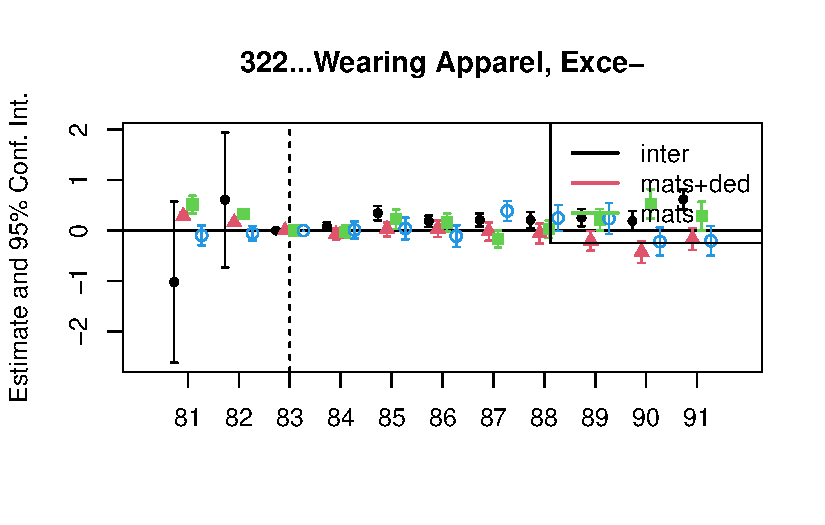
\includegraphics{Tax-Prod_files/figure-pdf/unnamed-chunk-11-1.pdf}

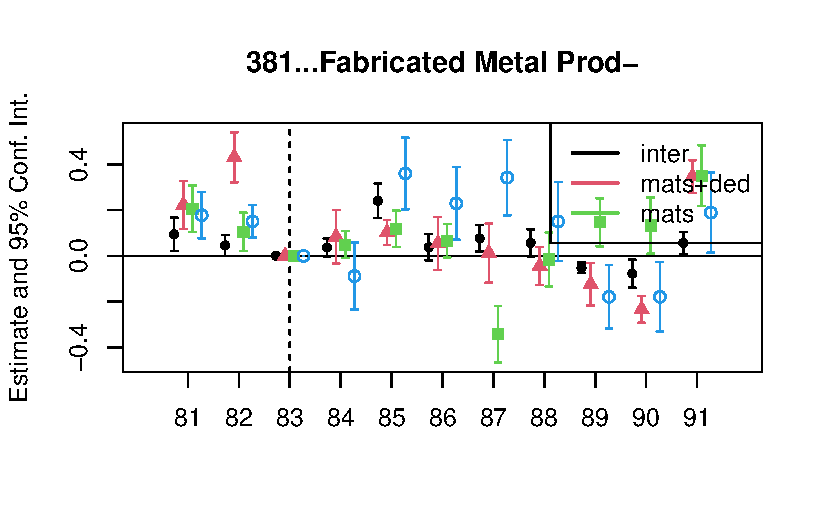
\includegraphics{Tax-Prod_files/figure-pdf/unnamed-chunk-11-2.pdf}

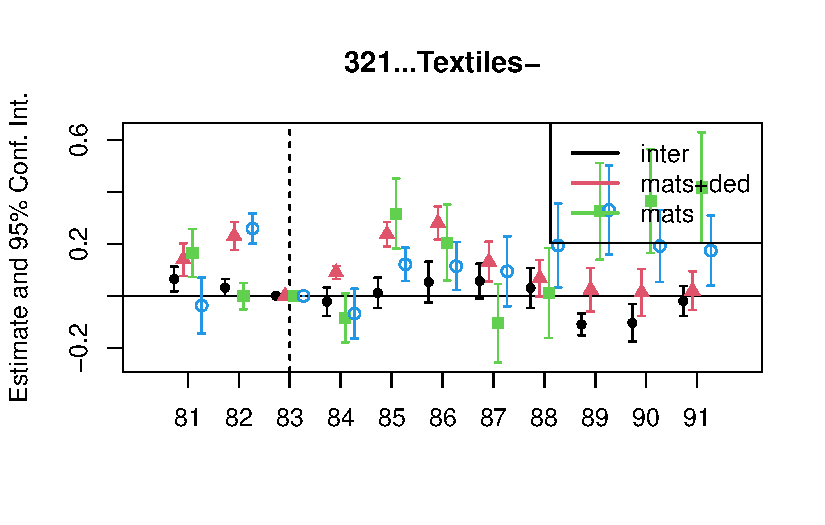
\includegraphics{Tax-Prod_files/figure-pdf/unnamed-chunk-11-3.pdf}

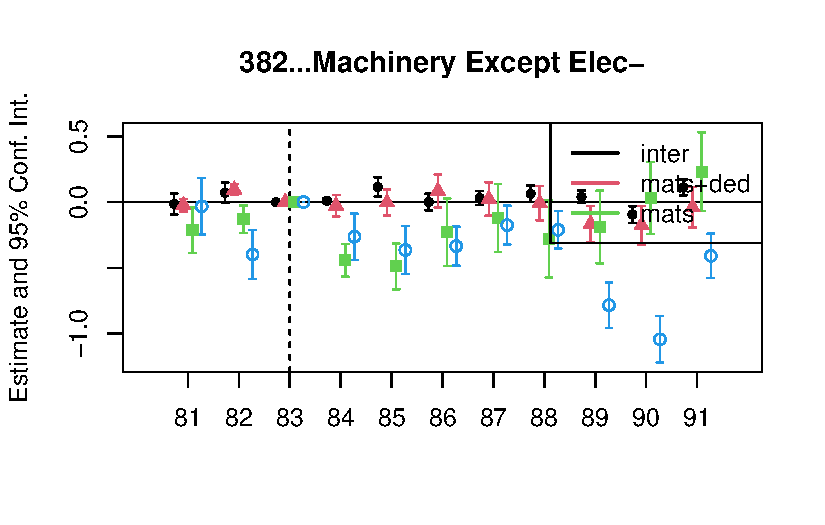
\includegraphics{Tax-Prod_files/figure-pdf/unnamed-chunk-11-4.pdf}

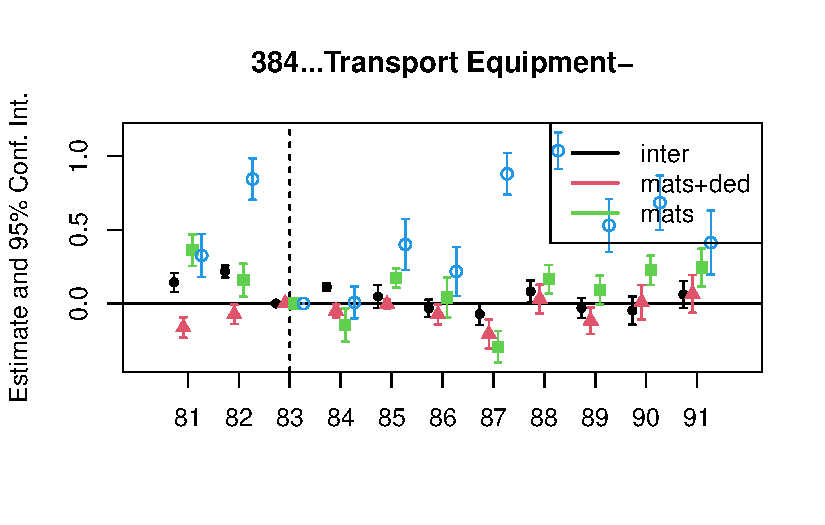
\includegraphics{Tax-Prod_files/figure-pdf/unnamed-chunk-11-5.pdf}

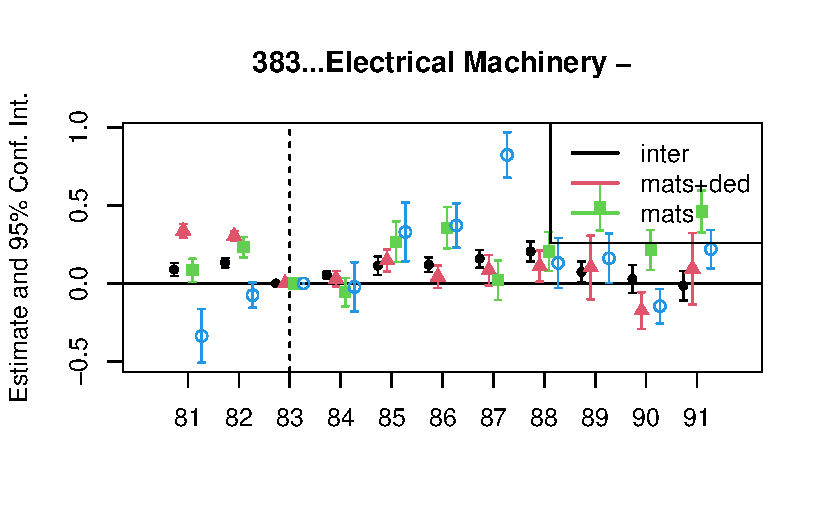
\includegraphics{Tax-Prod_files/figure-pdf/unnamed-chunk-11-6.pdf}

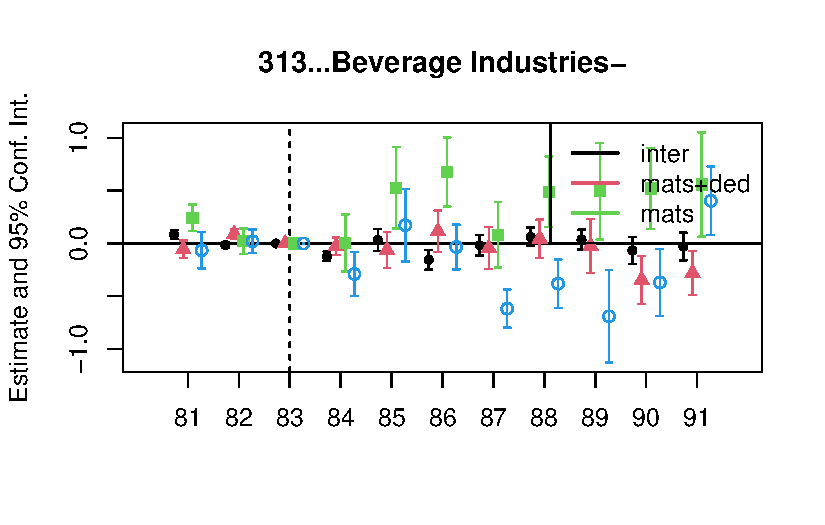
\includegraphics{Tax-Prod_files/figure-pdf/unnamed-chunk-11-7.pdf}

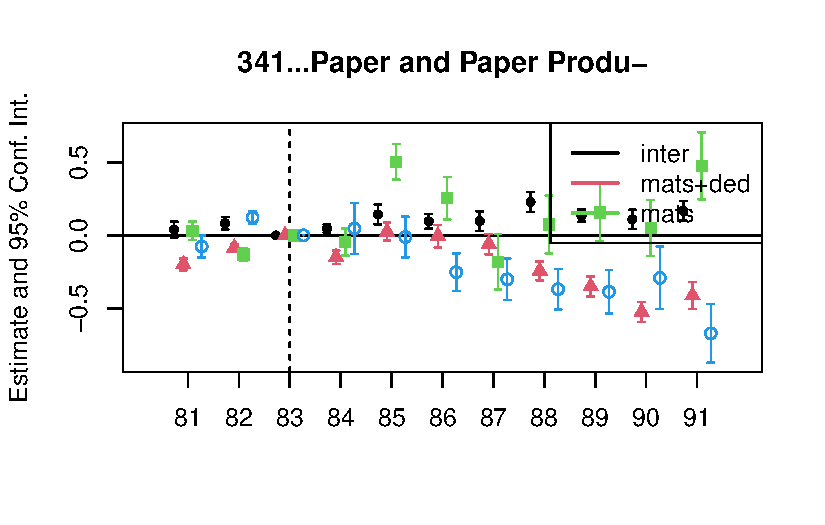
\includegraphics{Tax-Prod_files/figure-pdf/unnamed-chunk-11-8.pdf}

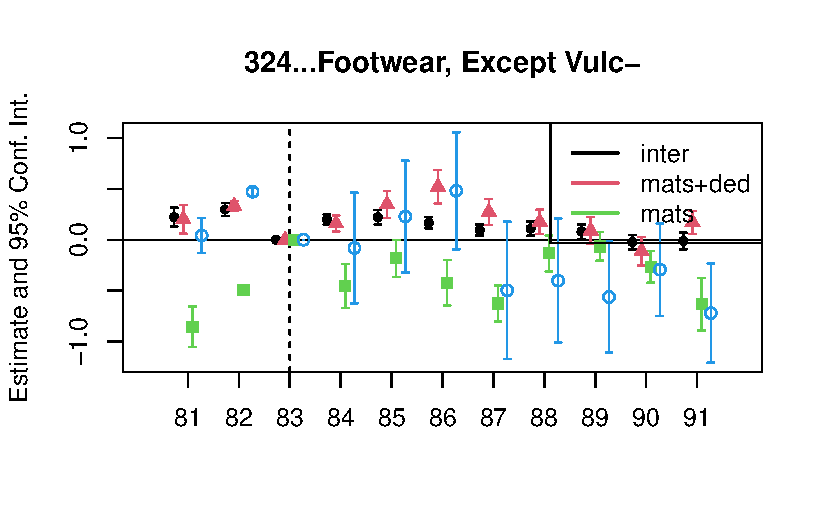
\includegraphics{Tax-Prod_files/figure-pdf/unnamed-chunk-11-9.pdf}

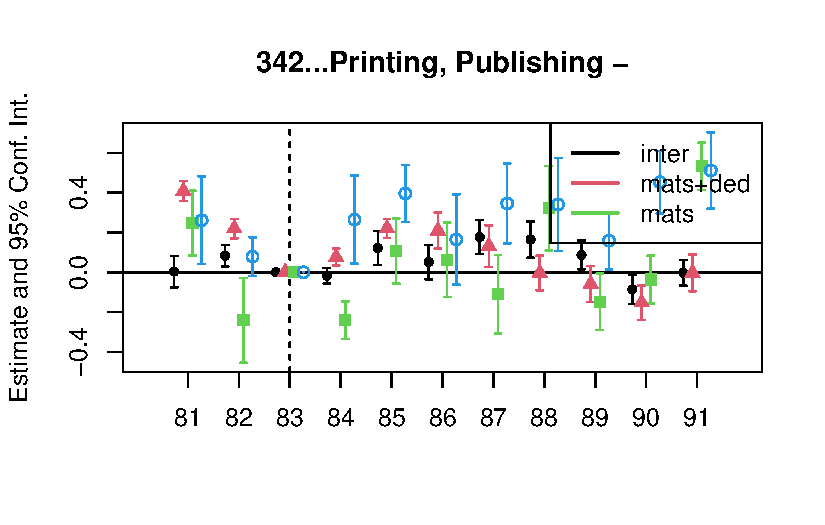
\includegraphics{Tax-Prod_files/figure-pdf/unnamed-chunk-11-10.pdf}

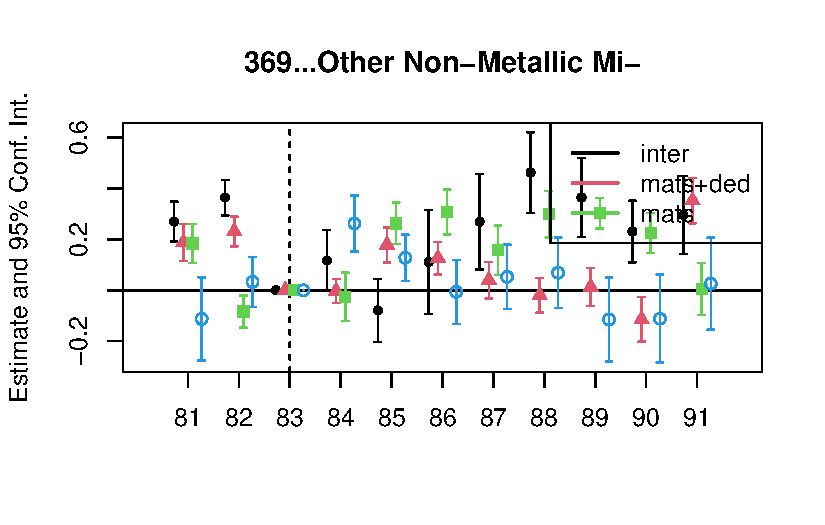
\includegraphics{Tax-Prod_files/figure-pdf/unnamed-chunk-11-11.pdf}

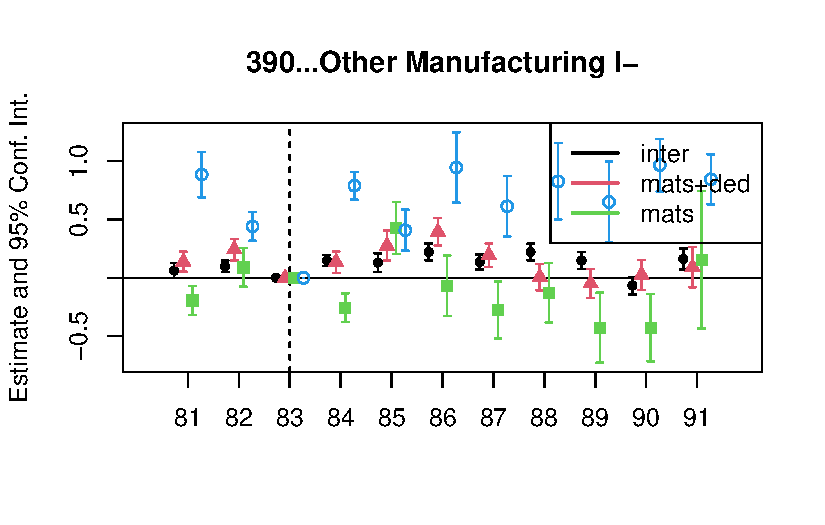
\includegraphics{Tax-Prod_files/figure-pdf/unnamed-chunk-11-12.pdf}

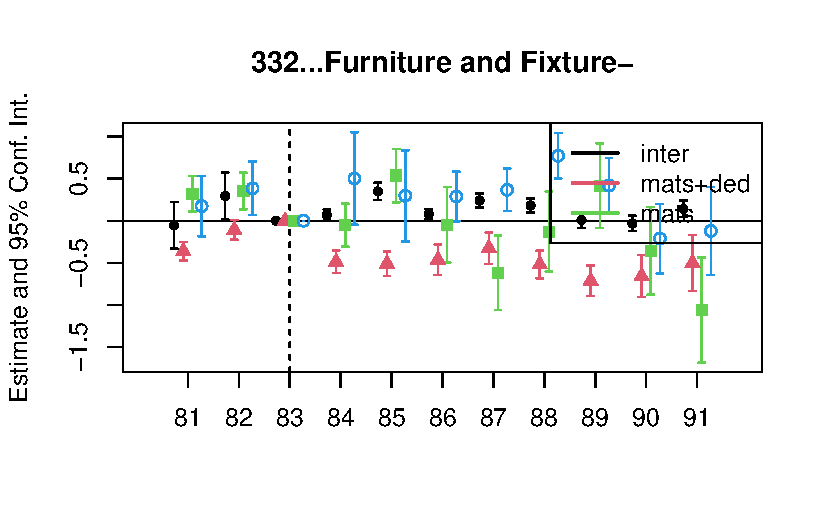
\includegraphics{Tax-Prod_files/figure-pdf/unnamed-chunk-11-13.pdf}

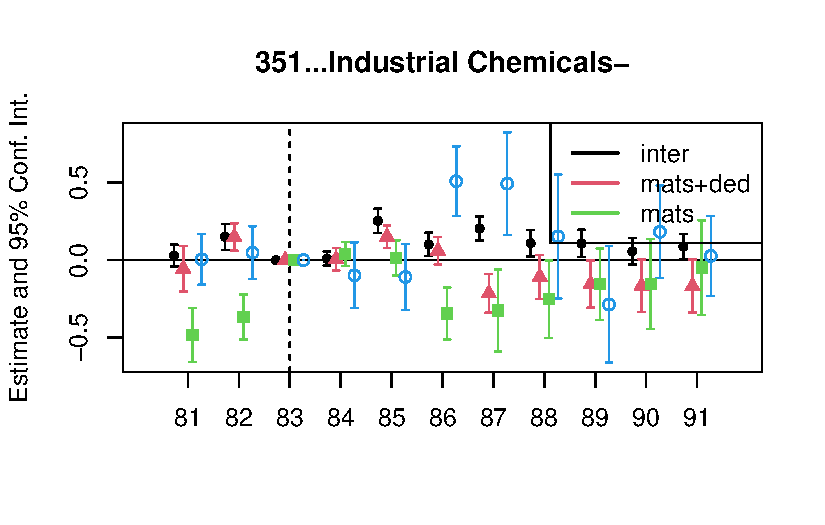
\includegraphics{Tax-Prod_files/figure-pdf/unnamed-chunk-11-14.pdf}

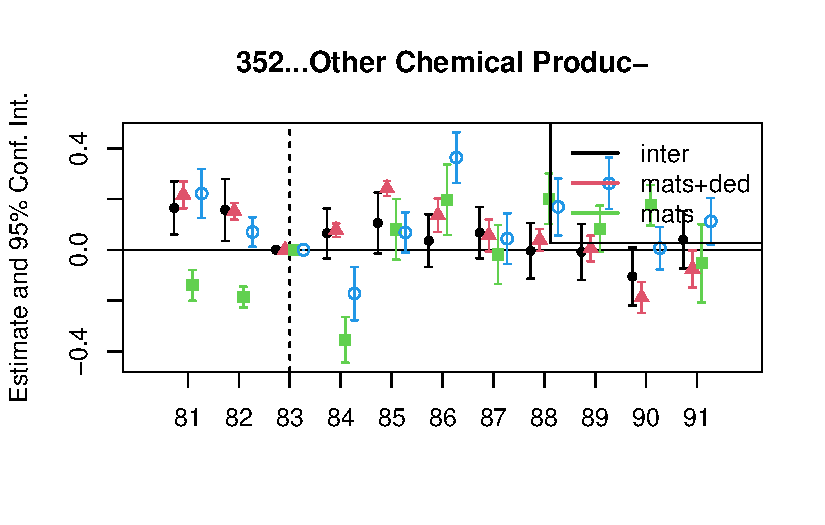
\includegraphics{Tax-Prod_files/figure-pdf/unnamed-chunk-11-15.pdf}

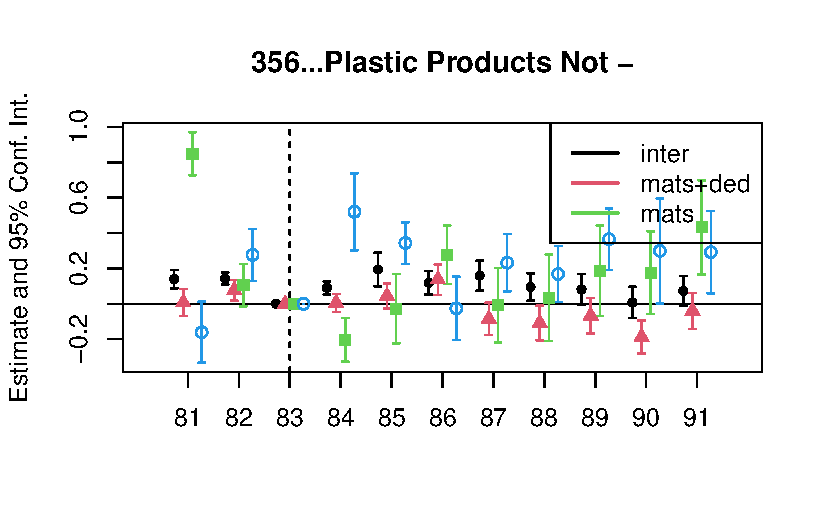
\includegraphics{Tax-Prod_files/figure-pdf/unnamed-chunk-11-16.pdf}

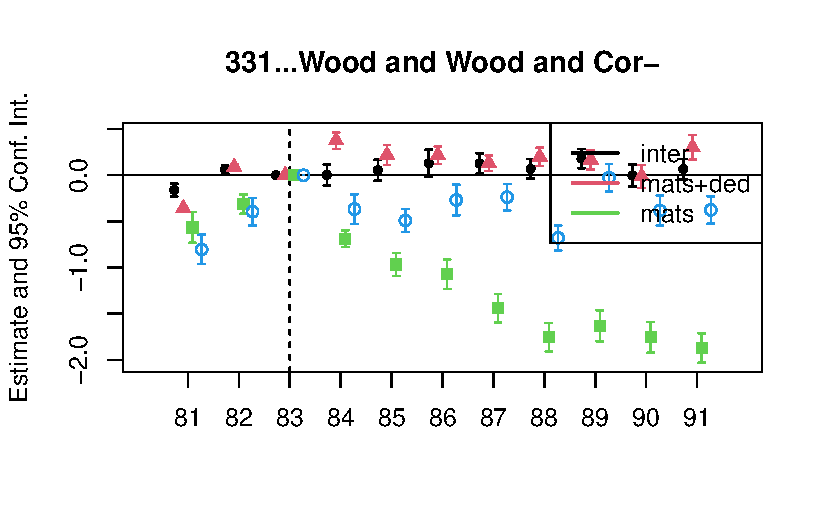
\includegraphics{Tax-Prod_files/figure-pdf/unnamed-chunk-11-17.pdf}

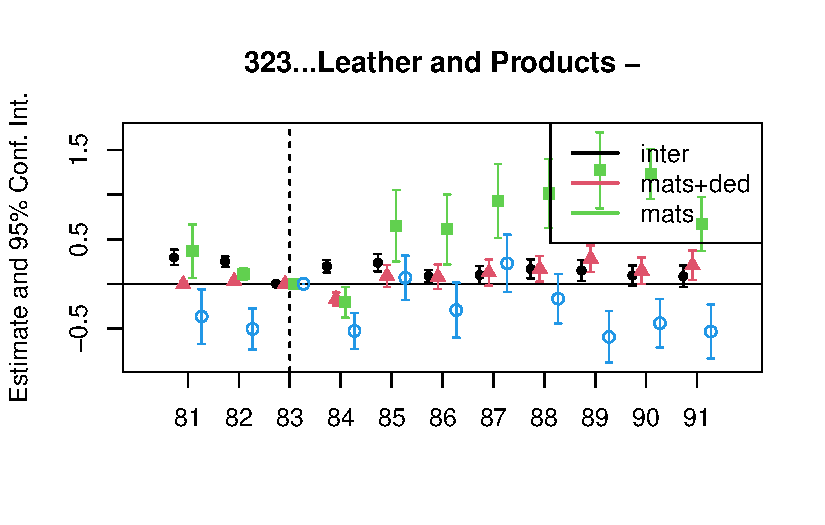
\includegraphics{Tax-Prod_files/figure-pdf/unnamed-chunk-11-18.pdf}

\end{minipage}%

\end{figure}%

\section{Empirical Appendix}\label{empirical-appendix}

\subsection{Changes in Sales Tax}\label{changes-in-sales-tax}

\begin{table}

\caption{\label{tbl-reg-did-inds}DiD on Sales Taxes by Industry. The
Control Group is Corporations in 1983 (1982).}

\begin{minipage}{\linewidth}

\begingroup
\centering
\begin{tabular}{lcccc}
   \tabularnewline \midrule \midrule
   Dependent Variable: & \multicolumn{4}{c}{Sales Tax Rate}\\
   Industry                 & 311                     & 312                     & 322             & 381 \\   
   Tax Change & \multicolumn{2}{c}{exempt} & \multicolumn{2}{c}{increased} \\ 
   Model:                   & (1)                     & (2)                     & (3)             & (4)\\  
   \midrule
   \emph{Variables}\\
   1984                     & -0.0001                 & -0.0007$^{***}$         & 0.0351$^{***}$  & -0.0018$^{**}$\\   
                            & ($8.27\times 10^{-5}$)  & ($5.57\times 10^{-5}$)  & (0.0012)        & (0.0007)\\   
   1985                     & -0.0005$^{***}$         & -0.0017$^{***}$         & 0.0408$^{***}$  & -0.0014$^{*}$\\   
                            & (0.0002)                & (0.0002)                & (0.0017)        & (0.0007)\\   
   1986                     & -0.0005$^{**}$          & -0.0026$^{***}$         & 0.0382$^{***}$  & 0.0017\\   
                            & (0.0002)                & (0.0002)                & (0.0020)        & (0.0011)\\   
   Non-Corp.                & 0.0015                  & -0.0020$^{***}$         & 0.0009          & 0.0076\\   
                            & (0.0008)                & (0.0006)                & (0.0026)        & (0.0056)\\   
   1984 $\times$ Non-Corp.  & -0.0004$^{**}$          & -0.0001                 & -0.0038$^{***}$ & 0.0020$^{**}$\\   
                            & (0.0001)                & (0.0002)                & (0.0012)        & (0.0007)\\   
   1985 $\times$ Non-Corp.  & -0.0003                 & 0.0018$^{***}$          & -0.0021         & 0.0101$^{***}$\\   
                            & (0.0003)                & (0.0003)                & (0.0018)        & (0.0006)\\   
   1986 $\times$ Non-Corp.  & $8.2\times 10^{-5}$     & 0.0036$^{***}$          & 0.0013          & 0.0083$^{***}$\\   
                            & (0.0002)                & (0.0001)                & (0.0021)        & (0.0011)\\   
   \midrule
   \emph{Fixed-effects}\\
   plant                    & Yes                     & Yes                     & Yes             & Yes\\  
   \midrule
   \emph{Fit statistics}\\
   Observations             & 6,074                   & 1,207                   & 4,445           & 3,678\\  
   R$^2$                    & 0.83275                 & 0.82556                 & 0.81582         & 0.59553\\  
   Within R$^2$             & 0.00900                 & 0.02030                 & 0.67843         & 0.08036\\  
   \midrule \midrule
   \multicolumn{5}{l}{\emph{Clustered (Year) standard-errors in parentheses}}\\
   \multicolumn{5}{l}{\emph{Signif. Codes: ***: 0.01, **: 0.05, *: 0.1}}\\
\end{tabular}
\par\endgroup
\begingroup
\centering
\begin{tabular}{lcccc}
   \tabularnewline \midrule \midrule
   Dependent Variable: & \multicolumn{4}{c}{Sales Tax Rate}\\
   Industry                 & 321            & 382            & 384            & 383 \\   
   Tax Change & \multicolumn{4}{c}{increased} \\ 
   Model:                   & (1)            & (2)            & (3)            & (4)\\  
   \midrule
   \emph{Variables}\\
   1984                     & 0.0243$^{***}$ & 0.0091$^{***}$ & 0.0062$^{***}$ & 0.0140$^{***}$\\   
                            & (0.0009)       & (0.0008)       & (0.0014)       & (0.0014)\\   
   1985                     & 0.0341$^{***}$ & 0.0347$^{***}$ & 0.0284$^{***}$ & 0.0182$^{***}$\\   
                            & (0.0009)       & (0.0014)       & (0.0013)       & (0.0013)\\   
   1986                     & 0.0344$^{***}$ & 0.0407$^{***}$ & 0.0359$^{***}$ & 0.0200$^{***}$\\   
                            & (0.0010)       & (0.0018)       & (0.0021)       & (0.0010)\\   
   Non-Corp.                & -0.0030$^{*}$  & -0.0038        & -0.0117$^{*}$  & -0.0041\\   
                            & (0.0015)       & (0.0040)       & (0.0054)       & (0.0025)\\   
   1984 $\times$ Non-Corp.  & 0.0036$^{***}$ & 0.0126$^{***}$ & 0.0079$^{***}$ & 0.0003\\   
                            & (0.0009)       & (0.0007)       & (0.0015)       & (0.0012)\\   
   1985 $\times$ Non-Corp.  & 0.0048$^{***}$ & 0.0113$^{***}$ & 0.0104$^{***}$ & 0.0062$^{***}$\\   
                            & (0.0009)       & (0.0013)       & (0.0011)       & (0.0012)\\   
   1986 $\times$ Non-Corp.  & 0.0043$^{***}$ & 0.0006         & 0.0059$^{***}$ & 0.0027$^{***}$\\   
                            & (0.0009)       & (0.0014)       & (0.0018)       & (0.0007)\\   
   \midrule
   \emph{Fixed-effects}\\
   plant                    & Yes            & Yes            & Yes            & Yes\\  
   \midrule
   \emph{Fit statistics}\\
   Observations             & 2,784          & 2,154          & 1,433          & 1,391\\  
   R$^2$                    & 0.82334        & 0.58862        & 0.73492        & 0.61201\\  
   Within R$^2$             & 0.68415        & 0.36100        & 0.36902        & 0.28558\\  
   \midrule \midrule
   \multicolumn{5}{l}{\emph{Clustered (Year) standard-errors in parentheses}}\\
   \multicolumn{5}{l}{\emph{Signif. Codes: ***: 0.01, **: 0.05, *: 0.1}}\\
\end{tabular}
\par\endgroup
\begingroup
\centering
\begin{tabular}{lcccc}
   \tabularnewline \midrule \midrule
   Dependent Variable: & \multicolumn{4}{c}{Sales Tax Rate}\\
   Industry                 & 313             & 341            & 324             & 342 \\   
   Tax Change & \multicolumn{3}{c}{increased} & decreased \\ 
   Model:                   & (1)             & (2)            & (3)             & (4)\\  
   \midrule
   \emph{Variables}\\
   1984                     & -0.0011         & 0.0145$^{***}$ & 0.0351$^{***}$  & -0.0061$^{***}$\\   
                            & (0.0006)        & (0.0008)       & (0.0019)        & (0.0010)\\   
   1985                     & 0.0641$^{***}$  & 0.0218$^{***}$ & 0.0527$^{***}$  & -0.0158$^{***}$\\   
                            & (0.0009)        & (0.0015)       & (0.0027)        & (0.0018)\\   
   1986                     & 0.0504$^{***}$  & 0.0206$^{***}$ & 0.0504$^{***}$  & -0.0123$^{***}$\\   
                            & (0.0018)        & (0.0009)       & (0.0029)        & (0.0028)\\   
   Non-Corp.                & 0.0251$^{*}$    & 0.0021         & 0.0118$^{**}$   & -0.0066$^{**}$\\   
                            & (0.0131)        & (0.0034)       & (0.0050)        & (0.0026)\\   
   1984 $\times$ Non-Corp.  & -0.0213$^{***}$ & 0.0021$^{*}$   & -0.0061$^{***}$ & -0.0089$^{***}$\\   
                            & (0.0012)        & (0.0011)       & (0.0018)        & (0.0010)\\   
   1985 $\times$ Non-Corp.  & -0.0657$^{***}$ & 0.0029         & -0.0139$^{***}$ & 0.0073$^{***}$\\   
                            & (0.0026)        & (0.0017)       & (0.0025)        & (0.0018)\\   
   1986 $\times$ Non-Corp.  & -0.0443$^{***}$ & 0.0061$^{***}$ & -0.0115$^{***}$ & 0.0033\\   
                            & (0.0027)        & (0.0014)       & (0.0025)        & (0.0030)\\   
   \midrule
   \emph{Fixed-effects}\\
   plant                    & Yes             & Yes            & Yes             & Yes\\  
   \midrule
   \emph{Fit statistics}\\
   Observations             & 978             & 1,072          & 1,074           & 2,003\\  
   R$^2$                    & 0.83712         & 0.68799        & 0.79885         & 0.86316\\  
   Within R$^2$             & 0.57436         & 0.40323        & 0.66598         & 0.11522\\  
   \midrule \midrule
   \multicolumn{5}{l}{\emph{Clustered (Year) standard-errors in parentheses}}\\
   \multicolumn{5}{l}{\emph{Signif. Codes: ***: 0.01, **: 0.05, *: 0.1}}\\
\end{tabular}
\par\endgroup
\begingroup
\centering
\begin{tabular}{lcccc}
   \tabularnewline \midrule \midrule
   Dependent Variable: & \multicolumn{4}{c}{Sales Tax Rate}\\
   Industry                 & 369             & 390             & 332             & 351 \\   
   Tax Change & \multicolumn{4}{c}{decreased} \\ 
   Model:                   & (1)             & (2)             & (3)             & (4)\\  
   \midrule
   \emph{Variables}\\
   1984                     & -0.0266$^{***}$ & -0.0189$^{***}$ & -0.0386$^{***}$ & -0.0192$^{***}$\\   
                            & (0.0010)        & (0.0026)        & (0.0059)        & (0.0008)\\   
   1985                     & -0.0294$^{***}$ & -0.0189$^{***}$ & -0.0378$^{***}$ & -0.0203$^{***}$\\   
                            & (0.0020)        & (0.0027)        & (0.0046)        & (0.0007)\\   
   1986                     & -0.0249$^{***}$ & -0.0169$^{***}$ & -0.0172$^{**}$  & -0.0254$^{***}$\\   
                            & (0.0026)        & (0.0029)        & (0.0064)        & (0.0014)\\   
   Non-Corp.                & -0.0102$^{*}$   & 0.0367$^{***}$  & -0.0086         & 0.0040\\   
                            & (0.0053)        & (0.0103)        & (0.0075)        & (0.0055)\\   
   1984 $\times$ Non-Corp.  & 0.0184$^{***}$  & 0.0045          & 0.0109$^{**}$   & 0.0020$^{**}$\\   
                            & (0.0009)        & (0.0028)        & (0.0044)        & (0.0007)\\   
   1985 $\times$ Non-Corp.  & 0.0143$^{***}$  & 0.0034          & 0.0128$^{***}$  & 0.0077$^{***}$\\   
                            & (0.0022)        & (0.0032)        & (0.0028)        & (0.0018)\\   
   1986 $\times$ Non-Corp.  & 0.0203$^{***}$  & 0.0017          & -0.0058         & 0.0095$^{***}$\\   
                            & (0.0031)        & (0.0031)        & (0.0042)        & (0.0025)\\   
   \midrule
   \emph{Fixed-effects}\\
   plant                    & Yes             & Yes             & Yes             & Yes\\  
   \midrule
   \emph{Fit statistics}\\
   Observations             & 1,932           & 998             & 992             & 787\\  
   R$^2$                    & 0.50882         & 0.68447         & 0.60906         & 0.81895\\  
   Within R$^2$             & 0.07690         & 0.12984         & 0.21598         & 0.12312\\  
   \midrule \midrule
   \multicolumn{5}{l}{\emph{Clustered (Year) standard-errors in parentheses}}\\
   \multicolumn{5}{l}{\emph{Signif. Codes: ***: 0.01, **: 0.05, *: 0.1}}\\
\end{tabular}
\par\endgroup

\end{minipage}%

\end{table}%

\section{Changes in Relative Prices}\label{changes-in-relative-prices}

An alternative hypothesis is that changes in the sales taxes change the
relative prices of inputs. It could be that the regressions are
capturing not the changes in evasion by overreporting but the changes in
relative prices.

Suppose we have two flexible inputs \(M\) and \(L\). \(M\) is deductible
but \(L\) is not. Equation~\ref{eq-eva} becomes then,

\begin{equation}\phantomsection\label{eq-eva-non-deduct}{
\begin{aligned}
  \max_{M_{it}, L_{it},e_{it}\in [0,\infty), } [1-q(e_{it}|\theta_{it})]&\left[P_t\mathbb{E}[Y_{it}]-\rho_{t} M_{it}-w_{t} L_{it}-\tau\left(P_t\mathbb{E}[Y_{it}]-\rho_{t} (M_{it}+e_{it})\right)\right]\\
  +q(e_{it}|\theta_{it})&\left[(1-\tau)(P_t\mathbb{E}[Y_{it}]-\rho_{t} M_{it})-w_{t} L_{it}-\kappa(e)\right] \\
  \text{s.t. }\; Y_{it}=G(M_{it})&\exp(\omega_{it}+\varepsilon_{it})
\end{aligned}
}\end{equation}

In the case of Colombia, \(\theta\) is their juridical organization.
Assume firms choose their \(\theta\) before the start of the period.
I'll come to this decision later, but for now, it follows that
\(q(e|\theta)=q(e)\). In other words, firms cannot affect their
detection probability when choosing inputs.

The first-order conditions now yield the following. For deductible
flexible inputs, the optimality condition remains the same as
Equation~\ref{eq-foc:ind},

\begin{equation}\phantomsection\label{eq-foc:deduct}{
G_M(M_{it}, L_{it})\exp(\omega_{it})\mathcal{E}=\frac{\rho_{t}}{P_t}
}\end{equation}

However, for non-deductible flexible inputs, the sales tax induces a
distortion in the optimality condition.

\begin{equation}\phantomsection\label{eq-foc:non-deduct}{
G_L(M_{it}, L_{it})\exp(\omega_{it})\mathcal{E}=\frac{w_{t}}{(1-\tau)P_t}
}\end{equation}

Finally, the optimality condition for tax evasion becomes,

\begin{equation}\phantomsection\label{eq-foc-cont-e}{
[1-q(e_{it})]\frac{\rho_t}{P_t}\tau-q(e_{it})\kappa'(e_{it})=q'(e_{it})\left[\frac{\rho_t}{P_t}\tau e_{it} + \kappa(e_{it})\right]
}\end{equation}

What can we conclude? First, if the production function is a
Cobb-Douglas, then we can independently solve for each input. In this
case, changes in VAT or CIT would not affect the optimality condition of
deductible flexible inputs because it would not affect the relative
prices. Therefore, changes in the consumption of deductible flexible
inputs due to changes in VAT or CIT can only be explained by an increase
in the incentives to evade taxes by overreporting.

On the other hand, an increase in the VAT or CIT would increase the
relative prices of non-deductible flexible inputs, leading to a decrease
in their consumption.

Alternatively, if non-deductible flexible inputs become deductible the
distortion in the optimality condition induced by the VAT and CIT would
be eliminated. Eliminating the distortion would lead to a reduction of
the relative prices inducing a higher consumption of these inputs.

Second, if the production function is not Cobb-Douglas, then the firm
has to solve the system of equations. Theoretically, the changes in the
relative prices of the non-deductible flexible inputs might affect the
consumption of the deductible flexible inputs depending on whether these
inputs are complements or substitutes.

Empirically, however, if I can observe deductible inputs separately from
non-deductible inputs, I can still be able to run the share regression
to recover the input elasticity of output. The observed consumed
non-deductible inputs will capture the changes in relative prices.

If I want to run the share regression using the non-deductible flexible
inputs, I have to be careful to account for the distortion induced by
the changes in taxes. If I observe the sales taxes, I can still be able
to control for changes in sales taxes and run this regression.

Theoretically, we would have,

\[
\begin{aligned}
    \ln\left(\frac{\rho_{t}M_{it}}{P_tY_{it}}\right)&=\ln D^{\mathcal{E}}_M(M_{it}, L_{it})-\varepsilon_{it} \\
    \ln\left(\frac{w_{t}L_{it}}{(1-\tau)P_tY_{it}}\right)&=\ln D^{\mathcal{E}}_L(M_{it}, L_{it})-\varepsilon_{it}
\end{aligned}
\]

Note that while we can use the gross revenue of sales for deductible
flexible inputs, we would have to use the net of tax sales revenues for
non-deductible flexible inputs.

More imporantly, note that the practicioner observes only
\(\ln M=\ln M^*+e\) but not \(M^*\). In section
Section~\ref{sec-id-strat}, I show how to recover these functions.

\section{Do Corporations in Colombia have different technologies than
other juridical
organizations?}\label{do-corporations-in-colombia-have-different-technologies-than-other-juridical-organizations}

An implicit assumption in the identification strategy is that the subset
of non-evaders has the same common technology as evaders. In the case of
Colombia, this implies that Corporations have the same common technology
as Proprietorships, Limited Companies, and Partnerships. However, we can
think that firms with better technology are self-selecting into
corporations, and thus, firms with low-performance technology will be
mislabeled as evaders.

The key question is how firms are choosing their juridical organization,
and in particular, how firms are choosing to become corporations. I
argue that choosing the juridical organization is a result of the
capital needs of the firm and it is affected by the preferences of the
owners over their corporate liability and their social connections.

From the definitions of the juridical organizations, we can expect
corporations to be the largests in terms of capital, followed by LLCs
and Partnerships, and Proprietorships to be smallest. The reason is
simply that more people can participate by contributing their capital to
the firm. This ordering in turn would suggest a growth path for the
firms.

Turning to the data, I find some firms change their juridical
organization type. I build a juridical organization transition matrix
from the previous year to the next one at the firm level.
Table~\ref{tbl-trans-mat} shows the transition matrix. Although the
transition matrix suggests that firms mostly stay in their juridical
organization, a growth trend emerges. It looks like proprietorships turn
into LLCs, and LLCs into Corporations.

\begin{table}

\caption{\label{tbl-trans-mat}Transition Matrix}

\centering{

\centering
\begin{tabular}[t]{l|r|r|r|r|r}
\hline
  & Proprietorship & Partnership & Ltd. Co. & Corporation & Total\\
\hline
Proprietorship & 94.8 & 0.7 & 4.5 & 0.1 & 4404\\
\hline
Partnership & 0.5 & 92.7 & 5.6 & 1.3 & 1241\\
\hline
Ltd. Co. & 0.2 & 0.1 & 98.6 & 1.0 & 22154\\
\hline
Corporation & 0.0 & 0.1 & 0.5 & 99.4 & 7805\\
\hline
\end{tabular}

}

\end{table}%

Looking into the capital distributions of proprietorships, LLCs, and
corporations we find that corporations are the largest, followed by
LLCs, and proprietorships are the smallest
Figure~\ref{fig-k-rev-hist-1}. However, there are considerable overlaps.
The same is true for revenues (in logs) Figure~\ref{fig-k-rev-hist-2}.
This is not surprising, as the need for larger capital increases, the
more people would need to participate.

However, when we look at the frequency distributions of the capital over
revenue ratio in logs, the distributions perfectly overlap
Figure~\ref{fig-k-rev-hist-3}. If corporations had different
technologies we would expect to see two different distributions. In
particular, the distribution of corporations would have been farther to
the right than the distributions of proprietorships and LLCs.

These patterns remain even after controlling for industry, metropolitan
area, and year Table~\ref{tbl-reg-choosing-jo}.

\begin{figure}

\begin{minipage}{0.50\linewidth}

\centering{

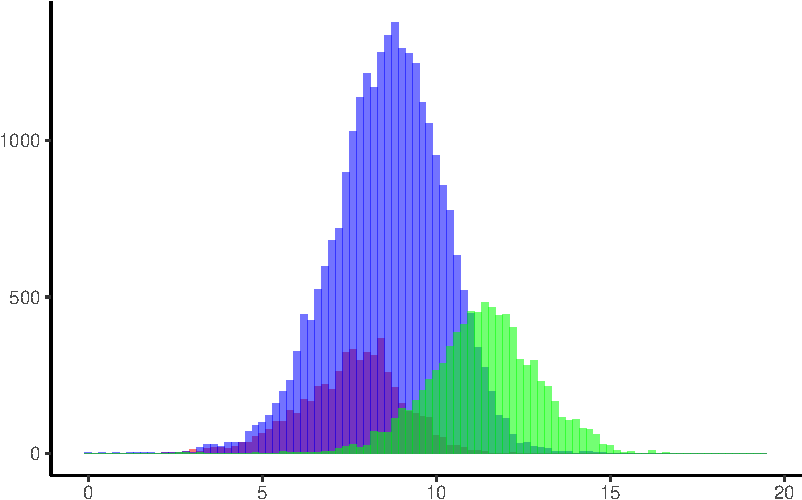
\includegraphics{Tax-Prod_files/figure-pdf/fig-k-rev-hist-1.pdf}

}

\subcaption{\label{fig-k-rev-hist-1}Capital}

\end{minipage}%
%
\begin{minipage}{0.50\linewidth}

\centering{

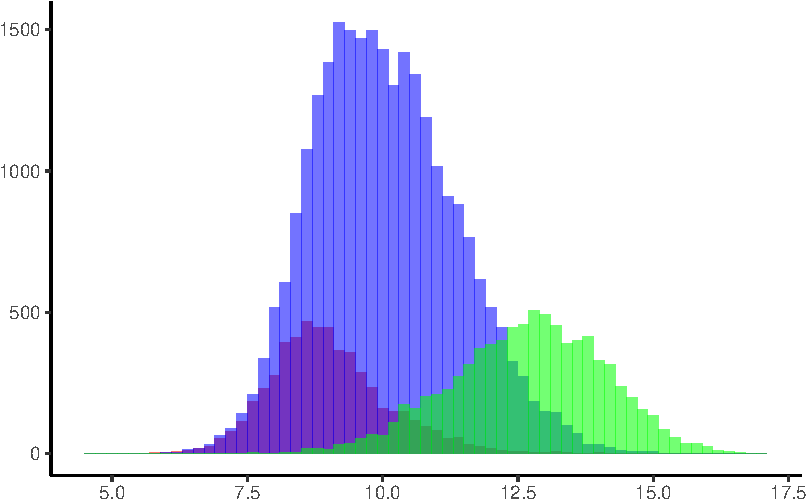
\includegraphics{Tax-Prod_files/figure-pdf/fig-k-rev-hist-2.pdf}

}

\subcaption{\label{fig-k-rev-hist-2}Revenue}

\end{minipage}%
\newline
\begin{minipage}{\linewidth}

\centering{

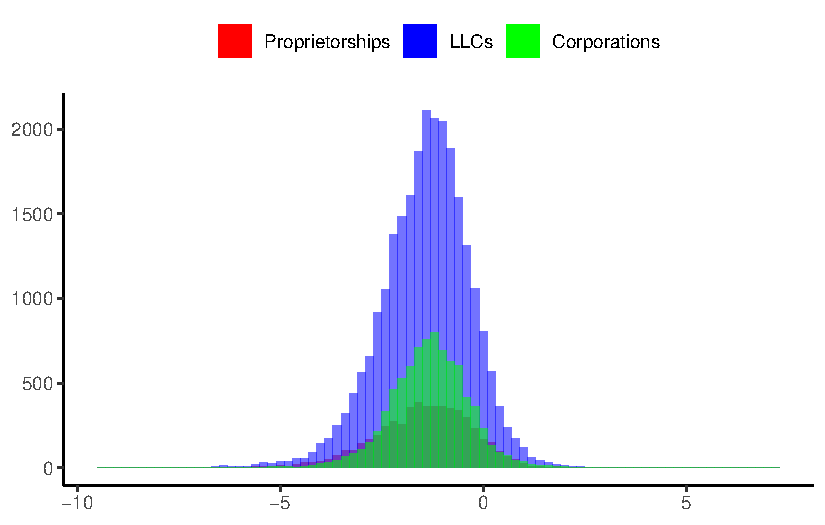
\includegraphics{Tax-Prod_files/figure-pdf/fig-k-rev-hist-3.pdf}

}

\subcaption{\label{fig-k-rev-hist-3}Capital/Revenue}

\end{minipage}%

\caption{\label{fig-k-rev-hist}Frequency historgrams of capital, revenue
and capital/revenue (in logs) of Corporations, LLCs, and
Proprietorships.}

\end{figure}%

\begin{table}

\caption{\label{tbl-reg-choosing-jo}Testing Differences in the log of
Capital, Revenue, and Capital/Revenue for Corporations and Other
Juridical Organizations}

\begin{minipage}{\linewidth}

\begingroup
\centering
\begin{tabular}{lccc}
   \tabularnewline \midrule \midrule
   Dependent Variables: & log(capital)   & log(sales)     & log(capital/sales)\\  
   Model:               & (1)            & (2)            & (3)\\  
   \midrule
   \emph{Variables}\\
   LLC                  & -2.446$^{***}$ & -2.424$^{***}$ & -0.0212\\   
                        & (0.0743)       & (0.0639)       & (0.0601)\\   
   Proprietorship       & -3.346$^{***}$ & -3.372$^{***}$ & 0.0265\\   
                        & (0.1672)       & (0.1220)       & (0.0897)\\   
   \midrule
   \emph{Fixed-effects}\\
   Industry             & Yes            & Yes            & Yes\\  
   Metro Area           & Yes            & Yes            & Yes\\  
   Year                 & Yes            & Yes            & Yes\\  
   \midrule
   \emph{Fit statistics}\\
   Observations         & 39,628         & 39,628         & 39,628\\  
   R$^2$                & 0.44574        & 0.51147        & 0.12003\\  
   Within R$^2$         & 0.31430        & 0.39972        & 0.00025\\  
   \midrule \midrule
   \multicolumn{4}{l}{\emph{Clustered (Industry \& Year) standard-errors in parentheses}}\\
   \multicolumn{4}{l}{\emph{Signif. Codes: ***: 0.01, **: 0.05, *: 0.1}}\\
\end{tabular}
\par\endgroup

\end{minipage}%

\end{table}%

\subsubsection{Model of firm (capital) growth
(sketch)}\label{model-of-firm-capital-growth-sketch}

A limited liability company looking to acquire more capital had three
options.

First, partners can increase their capital participation, using personal
wealth or through a bank credit. This option however will increase the
partners' liability. The more capital I bring the greater my liability
is.

Second, the LLC might increase its capital by inviting additional
partners. As the firm increases its capital, inviting more partners will
become more difficult. The funding partners risk losing control of their
firm, as more people participate in the firm's management and
decision-making.

Third, the firm can incorporate. This will bring capital to the firm.
Anyone in the market for the shares of the firm can participate. Shares
can be traded. A CEO reporting to the shareholders might be appointed.
Liability is limited to shares.

The decision to incorporate is a decision on how to acquire capital.
Firms still need to consider the stream of future productivity shocks,
but the decision also depends on other unobservables such as
risk-aversion (increasing the partners' liability), the partners'
ability to convince more partners to join the LLC, and preferences over
the control of the firm's management.

Assume there's an unobserved scalar \(\zeta_i\) that captures all of the
owners' heterogeneity in preferences over liability risk, access to
networks of potential investors, and preferences over the control of the
firm's management. Let a higher value of \(\zeta\) capture less risk
aversion, a wider network of potential investors, or a higher preference
for retaining control over the firm. Consider the case in which two LLCs
firms are looking to optimally increase their capital by the same
quantity, but the owners are different in \(\zeta\). In particular, let
the owner of firm 1 have a higher \(\zeta_1>\zeta_2\) than the owner of
firm 2. The firms also have the same technology and productivity shocks.
The owner of firm 1 \(\zeta_1\) would be able to convince additional
investors to join their LLC, but the owner 2 \(\zeta_2\) would not.
\(\zeta_2\) owner would have to choose to incorporate to get the capital
for his firm or forgo growth.

The 20 pp difference in CIT rate between LLCs and Corporations might
have deterred firm growth. The CIT was homogenized to 30\% in 1986. What
was the capital misallocation due to the tax rate differential? Are more
firms incorporating after the reform?

\subsubsection{Evasion vs.~Production
Technology}\label{evasion-vs.-production-technology}

Production technology is industry-specific, but evasion technology is
the same across industries.

Take the face value of the regressions and assume, without conceding,
that corporations have different technologies. This will imply that
corporations have technologies that are consistently 15\% more
productive than non-corporations regardless of the industry. In other
words, it does not matter if the firms produce canned food, shoes or
furniture, corporations have technologies consistently more productive.
However, this is difficult to believe because there could be industries
in which such an improvement in technology is difficult to imagine. For
example, coffee grain mills (food products), steel foundries (steel
basic products), plastic molding and extrusion (plastic products), or
cement (non-metallic mineral products).

However, these cross-sectional differences across industries could be
better explained by the evasion technology. We would expect the evasion
technology to be the same across industries. It does not matter what I
produce and what technology my firm employs, to overreport inputs all
that is needed is a fake invoice.

\subsubsection{Inputs Cost Share of
Revenues}\label{inputs-cost-share-of-revenues}

The evidence suggests that Corporations have similar technologies to the
rest of the firms. I look at the share of revenues of different input
costs. In doing so, I consider the incentives generated by the fiscal
environment in Colombia. Firms had the lowest incentives to evade taxes
by misreporting capital, consumed energy, and skilled labor. The cost
share of revenue of these inputs suggests that Corporations and the rest
of the firms had the same technologies.

\paragraph{Capital}\label{capital}

Firms could not deduct capital goods from sales taxes. However, firms of
capital-intensive industries might have had incentives to underreport
capital because capital was used to set the minimum income tax. Income
tax could not be less than 8 percent of the capital.

\paragraph{Energy}\label{energy}

Before the electrical energy reform in 1994, the power market was almost
exclusively supplied by public companies with negligible participation
from private firms. The public companies were inefficient and suffered
financial distress due to poor management and low tariffs set by
political actors. Two major blackouts in 1983 and 1992-1993 led to the
1994 reform that opened the sector to private participation.

It is unlikely that firms overreported energy, as they have to purchase
from a Corporation or a public company. Both of those organizations had
no incentives to cooperate and provide fake invoices.

In the data, energy sold by corporations accounted on average for 73\%
of the total energy sold, but only 1.7\% of the total energy purchased.
In addition, corporations sold energy at 12 times the market price on
average Table~\ref{tbl-energy}. The high price might suggest
corporations had market power in the electric energy market, however,
this is unlikely to be relevant to affect any estimations as their
overall market share is small.

\begin{table}

\caption{\label{tbl-energy}Electric energy market in Colombia
(1981-1991).}

\centering{

\centering
\begin{tabular}[t]{l|r|r|r|r}
\hline
 & Sold/Purchased Price Ratio & Sold Energy (\% of Total Sold Energy) & Sold Energy (\% of Total Purchased Energy) & Generated Energy (\% of Consumed Energy)\\
\hline
Corporation & 11.9 & 74.8 & 2.0 & 2.9\\
\hline
Ltd. Co. & 7.4 & 2.7 & 0.1 & 0.1\\
\hline
Other & 2.5 & 22.4 & 0.6 & 3.4\\
\hline
Partnership & 1.0 & 0.0 & 0.0 & 0.6\\
\hline
Proprietorship & 1.0 & 0.0 & 0.0 & 0.0\\
\hline
\end{tabular}

}

\end{table}%

\paragraph{Labor}\label{labor}

Firms might have incentives to underreport labor to evade Payroll Taxes
(PRT) if the expected benefits of evading the PRT outweigh the
opportunity costs of evading Corporate Income Tax (CIT) by overreporting
labor costs and the expected cost of evading PRT \citep{Almunia2018}.

Firms are more likely to underreport unskilled rather than skilled
labor. Skilled employees are less likely to cooperate with firms in
underreporting their wages. Firms might offer employees cash
compensations in order for employees to accept lower reported wages or
report their wages at all. The cost for employees is that these payroll
taxes provide them with social benefits such as social security or
public health access. These benefits are not obvious in the short run.
It is more likely that unskilled labor to be short-sighted and accept to
cooperate with firms to underreport their wages. Skilled workers, on the
other hand, are less likely to accept these conditions and to have
outside options and move if the conditions are not favorable to them.

\paragraph{Services and other
expenditures}\label{services-and-other-expenditures}

The Colombian dataset allows, to some extent, separating expenditures,
including services, into deductible and non-deductible expenses. In
contrast to non-evading firms, evading firms should use a higher share
of deductible expenses. The reason is that firms have incentives to
overreport deductible expenditure to evade ICT and VAT.

The Colombian data separates firms' total expenditures into general and
industrial expenditures. Industrial expenditure is defined as the
indirect costs and expenditures incurred by the firm in order to perform
its industrial activity. The data lists the purchase of accessories and
replacement parts, fuels and lubricants consumed by the establishment,
industrial work by other establishments, and third-party repairs and
maintenance, among others, as industrial expenditures\footnote{After
  1992, industrial expenditure included rent of machinery and property,
  payment for professional services, insurance (excluding employee
  benefits), water, mail, and telephone.}. All other expenses, including
insurance (excluding employee benefits) and machinery rentals, are
considered general expenses.

Most services were excluded from sales taxes. Some non-excluded services
in this period were insurance premiums (excluding life insurance),
repair and maintenance, national and international telegrams, telex, and
telephone, and rental of goods and chattels, including financial
leasing.

I classify as deductible expenses the following industrial expenditures:
purchase of fuels and lubricants, payments to third parties for repair
and maintenance, purchase of raw materials and goods sold without
transformation; and the following general expenditures: machinery
rental, insurance excluding employee benefits, and water, mail and
telephone expenses.

\paragraph{Technical note}\label{technical-note}

According to the notes on the dataset, the quantity of energy consumed
by firms is estimated as the difference between purchased plus generated
energy and sold energy. In contrast, the value of consumed energy is the
difference between the value of purchased and sold energy. Consequently,
using the calculated value over the calculated quantity of consumed
energy ignores the quantity of generated energy and the increase in the
price of sold energy by corporations.

In \citet{Gandhi2020}, services are defined as general expenditures
minus machinery rental and interest payments. However, this approach
does not include industrial expenditures which are closely linked to the
production process. In the Colombian data, the intermediate consumption
is defined as raw materials, purchased electric energy, and industrial
expenditure. This definition is close to what is commonly defined as
intermediate inputs.

\paragraph{Results}\label{results}

Table~\ref{tbl-reg-shares} shows that in terms of the capital and
consumed energy share of revenue, corporations are not different from
other types of juridical organizations. Capital and consumed energy are
reliable indicators that Corporations have similar technologies to other
firms because firms have no incentives to overreport capital or consumed
energy. On the other hand, the raw materials share of revenues is 3
percent higher for non-corporations. Firms have incentives to overreport
raw materials to evade sales taxes and CIT. Hence, materials are not a
good reference to compare technology between Corporations and other
types of firms.

Table~\ref{tbl-reg-shares-2} shows that the skilled labor share of
revenue for corporations is not statistically different from other types
of firms. On the other hand, unskilled labor is significantly lower for
non-corporations. Unskilled workers are more likely to cooperate with
non-corporations to underreport their employment/wages. An alternative
explanation is that corporations employ more unskilled workers because
they are bigger. Therefore, skilled labor is a more reliable indicator
of technology and shows that corporations have similar technology to
other firms.

Table~\ref{tbl-reg-shares-2} also shows that the total expenditure share
of revenue is 8 percent lower for non-corporations on average. On one
hand, this might be due to size. Corporations tend to be larger than
non-corporations. However, the composition of the expenditure matters.

Table~\ref{tbl-reg-shares-3} shows that the deductible expenses share of
total expenditure is 6 percent significantly higher for
non-corporations. This is not the case if we classify expenditures by
industrial and general expenses. Services as defined in GNR, that is
general expenses minus machinery rental and interest payments, as a
share of total expenditure is 5 percent higher for non-corporations.
Services include deductible expenses such as insurance excluding
employee benefits, and telegrams and telephone services.

In summary, looking at the inputs that firms are less likely to
misreport due to tax evasion incentives, the evidence suggests that
Corporations have similar technologies to the other types of firms. In
addition, I find that the cost share of inputs that are likely to be
misreported due to tax evasion incentives are significantly different
from corporations and in the expected direction. In particular, it looks
like firms overreport materials and deductible expenses, and underreport
unskilled labor.

\begin{table}

\caption{\label{tbl-reg-shares}Shares of Revenue for different inputs by
Corporations and Non-Corporation.}

\begin{minipage}{\linewidth}

\begingroup
\centering
\begin{tabular}{lccc}
   \tabularnewline \midrule \midrule
   Dependent Variables: & Capital               & energy\_share  & Materials\\  
   Model:               & (1)                   & (2)            & (3)\\  
   \midrule
   \emph{Variables}\\
   Non-Corporation      & 0.1524                & 0.0010         & 0.0252$^{**}$\\   
                        & (0.1063)              & (0.0019)       & (0.0092)\\   
   \midrule
   \emph{Fixed-effects}\\
   Industry             & Yes                   & Yes            & Yes\\  
   Metro Area           & Yes                   & Yes            & Yes\\  
   Year                 & Yes                   & Yes            & Yes\\  
   \midrule
   \emph{Fit statistics}\\
   Observations         & 42,145                & 41,774         & 42,145\\  
   R$^2$                & 0.00180               & 0.22196        & 0.01744\\  
   Within R$^2$         & $5.74\times 10^{-5}$  & 0.00011        & 0.00021\\  
   \midrule \midrule
   \multicolumn{4}{l}{\emph{Clustered (Industry \& Year) standard-errors in parentheses}}\\
   \multicolumn{4}{l}{\emph{Signif. Codes: ***: 0.01, **: 0.05, *: 0.1}}\\
\end{tabular}
\par\endgroup

\end{minipage}%

\end{table}%

\begin{table}

\caption{\label{tbl-reg-shares-2}Shares of Revenue for different inputs
by Corporations and Non-Corporation.}

\begin{minipage}{\linewidth}

\begingroup
\centering
\begin{tabular}{lccc}
   \tabularnewline \midrule \midrule
   Dependent Variables: & Skilled Labor         & Unskilled Labor & fuels\_share\\   
   Model:               & (1)                   & (2)             & (3)\\  
   \midrule
   \emph{Variables}\\
   Non-Corporation      & 0.2052                & 0.0740$^{***}$  & $-8.16\times 10^{-6}$\\    
                        & (0.2082)              & (0.0090)        & (0.0011)\\   
   \midrule
   \emph{Fixed-effects}\\
   Industry             & Yes                   & Yes             & Yes\\  
   Metro Area           & Yes                   & Yes             & Yes\\  
   Year                 & Yes                   & Yes             & Yes\\  
   \midrule
   \emph{Fit statistics}\\
   Observations         & 42,145                & 42,145          & 42,145\\  
   R$^2$                & 0.00186               & 0.02102         & 0.20652\\  
   Within R$^2$         & $1.91\times 10^{-5}$  & 0.00288         & $1.46\times 10^{-8}$\\   
   \midrule \midrule
   \multicolumn{4}{l}{\emph{Clustered (Industry \& Year) standard-errors in parentheses}}\\
   \multicolumn{4}{l}{\emph{Signif. Codes: ***: 0.01, **: 0.05, *: 0.1}}\\
\end{tabular}
\par\endgroup

\end{minipage}%

\end{table}%

\begin{table}

\caption{\label{tbl-reg-shares-3}Shares of Total Expenses for different
classifications of expenses by Corporations and Non-Corporation.}

\begin{minipage}{\linewidth}

\begingroup
\centering
\begin{tabular}{lccc}
   \tabularnewline \midrule \midrule
   Dependent Variables: & repair\_maint\_share   & services\_share  & inds\_nded\_share\\    
   Model:               & (1)                    & (2)              & (3)\\  
   \midrule
   \emph{Variables}\\
   Non-Corporation      & -0.0013                & -0.0341$^{***}$  & -0.0079$^{***}$\\   
                        & (0.0008)               & (0.0052)         & (0.0021)\\   
   \midrule
   \emph{Fixed-effects}\\
   Industry             & Yes                    & Yes              & Yes\\  
   Metro Area           & Yes                    & Yes              & Yes\\  
   Year                 & Yes                    & Yes              & Yes\\  
   \midrule
   \emph{Fit statistics}\\
   Observations         & 42,145                 & 42,145           & 42,145\\  
   R$^2$                & 0.07343                & 0.03208          & 0.06137\\  
   Within R$^2$         & 0.00112                & 0.00575          & 0.00607\\  
   \midrule \midrule
   \multicolumn{4}{l}{\emph{Clustered (Industry \& Year) standard-errors in parentheses}}\\
   \multicolumn{4}{l}{\emph{Signif. Codes: ***: 0.01, **: 0.05, *: 0.1}}\\
\end{tabular}
\par\endgroup

\end{minipage}%

\end{table}%

\section{Identification Strategy}\label{sec-id-strat}

Because the firms' optimization decisions depend on the fiscal
environment, the identification strategy should be motivated by the
fiscal environment \(\Gamma\). In particular, the identification
strategy will be as good as how well we can tell apart a subset of firms
that have the highest incentive to not evade. For example, in the case
of Spain, the firms above the revenue LTU threshold. In the case of
Colombia, the corporations.

\phantomsection\label{ass-non-ev}
\begin{fbx}{Assumption}{Assumption 8.1: }{Non-Evaders}
\phantomsection\label{ass-non-ev}
Based on the fiscal environment \(\Gamma\), the researcher can identify
a subset of firms \(\theta_i\in\Theta^{NE}\subset \Theta\) that does not
evade taxes by overreporting inputs.

\end{fbx}

For those firms, then \(\mathbb{E}[e_{it}|\theta_i\in\Theta^{NE}]=0\)

In addition, I impose the following timing assumption.

\phantomsection\label{ass-ind}
\begin{fbx}{Assumption}{Assumption 8.2: }{Independence}
\phantomsection\label{ass-ind}
Firms choose overreporting \(e_{it}\) \emph{before }the output shock
\(\varepsilon_{it}\)

\end{fbx}

Assumption \hyperref[ass-ind]{8.2} implies that input overreporting is
independent of the current period output shock,
\(e_{it} \perp \varepsilon_{it}\). In the literature is not rare to
assume that the output shock is not part of the information set of the
firms, \(\varepsilon_{it}\not\in \mathcal{I}_t\) \citep{Gandhi2020}.
Timing and information set assumptions are not uncommon for
identification strategies in production functions and demand estimation
\citep{Ackerberg2021, Ackerberg2019}.

\subsection{Identifying the production function
parameters}\label{identifying-the-production-function-parameters}

The econometrician observes then the overreported inputs in the data,
\(M_{it}=M^*_{it}\exp(e_{it})\)\footnote{Note we can always rewrite
  \(M^*+e=M^*\exp\{a\}\), then \(\exp\{a\}=\frac{e}{M^*}+1\).}. Assume
the production function is Cobb-Douglas,
\(G(M^*_{it}, K_{it}, L_{it})\exp(\omega_{it}+\varepsilon_{it})=M^{*\beta}_{it}K_{it}^{\alpha_K}L_{it}^{\alpha_L}\exp(\omega_{it}+\varepsilon_{it})\).
Then, for the case of Colombia, Equation~\ref{eq-foc:ind} applies since
the type of firms is the juridical organization and the non-evaders are
Corporations. By multiplying both sides by the intermediate inputs and
dividing by the output, we get

\begin{equation}\phantomsection\label{eq-foc-cd}{
\begin{aligned}
    \ln\left(\frac{\rho_t M^*_{it}}{P_{t}Y_{it}}\right)+e_{it}&=\ln\beta + \ln \mathcal{E}- \varepsilon_{it} \\
    &\equiv \ln D^{\mathcal{E}}- \varepsilon_{it} 
\end{aligned}
}\end{equation}

where,
\(\mathcal{E}\equiv \mathbb{E}[\exp(\varepsilon_{it})|\mathcal{I}_{it}]=\mathbb{E}[\exp(\varepsilon_{it})]\).

We can use Equation~\ref{eq-foc-cd} and assumption
\hyperref[ass-non-ev]{8.1} to recover the production function parameter
\(\beta\)

\begin{equation}\phantomsection\label{eq-foc-cd-exp}{
    \mathbb{E}\left[\ln\left(\frac{\rho_t M^*_{it}}{P_{t}Y_{it}}\right)\Bigg| \Theta^{NE}\right]=\ln D^{\mathcal{E}}
}\end{equation}

The constant \(\mathcal{E}\) is also identified \citep{Gandhi2020},

\begin{equation}\phantomsection\label{eq-id-E}{
\mathcal{E}=\mathbb{E}\left[\exp\left(\ln D^{\mathcal{E}}- \ln\left(\frac{\rho_t M^*_{it}}{P_{t}Y_{it}}\right)\right)|\theta^{NE}\right]=\mathbb{E}\left[\exp(\varepsilon_{it})|\theta^{NE}\right]=\mathbb{E}[\exp(\varepsilon_{it})]
}\end{equation}

and, thus, the output elasticity of input, \(\beta\), is also
identified,

\begin{equation}\phantomsection\label{eq-id-beta}{
\beta=\exp\left(\ln D^{\mathcal{E}}-\ln\mathcal{E}\right).
}\end{equation}

\subsection{Identifying Tax Evasion}\label{identifying-tax-evasion}

Having recovered both the flexible input elasticity, \(\beta\), and the
constant \(\mathcal{E}\), for all firms, I can form the following
variable using observed data.

\begin{equation}\phantomsection\label{eq-ob-ev}{
\begin{aligned}
    \mathcal V_{it}\equiv&\ln\left(\frac{\rho_t M_{it}}{P_{t}Y_{it}}\right)-\ln\beta -\ln\mathcal{E}\notag \\
    &=\ln\left(\frac{\rho_tM^*_{it}}{P_{t}Y_{it}}\right)-\ln\beta-\ln\mathcal{E}+e_{it} \notag \\
    &=-\varepsilon_{it} +e_{it}
\end{aligned}
}\end{equation}

Tax evasion therefore can be recovered up to an independent random
variable. We can do better however. By assumption
\hyperref[ass-ind]{8.2}, the tax evasion, \(\varepsilon_{it}\) ,is
independent of \(e_{it}\). Note that, from Equation~\ref{eq-foc-cd}, we
also recovered \(f_{\varepsilon}(\varepsilon)\) the distribution of
\(\varepsilon\). By using deconvolution methods, I can recover the tax
evasion apart from the output shock.

In particular, from probability theory,

\begin{definition}[]\protect\hypertarget{def-conv}{}\label{def-conv}

\begin{fbx}{Definition}{Definition: }{Convolution}
\phantomsection\label{}
The density of the sum of two \textbf{independent} random variables is
equal to the \textbf{convolution} of the densities of both addends;
hence

\[
h = f*m = \int f(\mathcal Z - \varepsilon)m(\varepsilon)d\varepsilon
\]

where \(f\) is the density of \(\mathcal Z\) (Meister, 2009)

\end{fbx}

\end{definition}

\subsection{Identifying Productivity}\label{identifying-productivity}

Here, I show how to recover the rest of the parameters of the production
function, including productivity and its Markov process. We can do it in
several ways, depending on our object of interest.

In the literature, it is not uncommon to assume that productivity
follows a Markov process. That is,

\begin{equation}\phantomsection\label{eq-prod-markov}{
    \omega_{it}=h(\omega_{it-1})+\eta_{it}
}\end{equation}

Let \(\ln X_{it}=x_{it}\). With Equation~\ref{eq-ob-ev}, we can form the
following observed variable,

\begin{equation}\phantomsection\label{eq-big-w}{
\begin{aligned}
    \mathcal W_{it} & \equiv y_{it} - \beta (m_{it}-\mathcal{V}_{it})\\
    & = y_{it} - \beta (m^*_{it}+e_{it}-\mathcal{V}_{it})\\
    & = \alpha_K k_{it}+\alpha_L l_{it}+\omega_{it}+(1-\beta)\varepsilon_{it}
\end{aligned}
}\end{equation}

Here, intuitively, we are trading unobservables, the unobserved tax
evasion for the output shock, just to make our lives easier. We could
have use use directly \(m^*\) since we know the distribution of tax
evasion \(e\), which is equivalent to the distribution of
\(f_{m^*|m}(m^*|m)\). Also note that is it not necessary to learn tax
evasion to recover productivity. This is useful if a practicioner is
only interested in productivity and not on tax evasion.

By replacing \(\omega_{it}\) from Equation~\ref{eq-big-w} in
Equation~\ref{eq-prod-markov}, we get

\begin{equation}\phantomsection\label{eq-big-w-reg}{
\begin{aligned}
    \mathcal W_{it}=(1-\beta)\varepsilon_{it}+\alpha_K k_{it}+\alpha_L l_{it}+h(\mathcal W_{it-1}-(1-\beta)\varepsilon_{it-1}-\alpha_K k_{it-1}-\alpha_L l_{it-1})+\eta_{it}
\end{aligned}
}\end{equation}

To learn \(\alpha\) and \(h\), we need to find instruments \(Z\) such
that, \[
\begin{aligned}    
 \mathbb{E}[&\mathcal{W}_{it}|Z_{it}]\\
 &=\alpha_K k_{it}+\alpha_L l_{it}+\mathbb{E}_{\varepsilon_{t-1}}\left[\mathbb{E}[ h(\mathcal W_{it-1}-(1-\beta)\varepsilon_{it-1}-\alpha_K k_{it-1}-\alpha_L l_{it-1})|Z_{it},\varepsilon_{t-1}]|Z_{it}\right]\\
 &=\alpha_K k_{it}+\alpha_L l_{it}\\
 &+\int\int h(\mathcal W_{it-1}-(1-\beta)\varepsilon_{it-1}-\alpha_K k_{it-1}-\alpha_L l_{it-1})f_{\mathcal{W}_{it}}(\mathcal{W}_{it}|Z_{it})f_{\varepsilon_{it-1}}(\varepsilon_{it-1})d\mathcal{W}_{it}d\varepsilon_{it-1}\\
 &=\alpha_K k_{it}+\alpha_L l_{it}+\mathbb{E}\left[\int h(\mathcal W_{it-1}-(1-\beta)\varepsilon_{it-1}-\alpha_K k_{it-1}-\alpha_L l_{it-1})f_{\varepsilon_{it-1}}(\varepsilon_{it-1})d\varepsilon_{it-1}|Z_{it}\right]\\
&=\alpha_K k_{it}+\alpha_L l_{it}+h(\mathcal W_{it-1}-(1-\beta)\varepsilon_{it-1}-\alpha_K k_{it-1}-\alpha_L l_{it-1})
\end{aligned}
\]

The first line should follow from the orthogonality of the output shock
\(\mathbb{E}[\varepsilon_{it}|Z_{it}]=0\) and the law of iterated
expectations. The second line should follow from the definition of
expectation and the independence of the output shock of the previous
period. The third line follows from the interchangeability of integrals.
Thus, \(\alpha\) and \(h\) are identified.

\begin{longtable}[]{@{}
  >{\raggedright\arraybackslash}p{(\columnwidth - 2\tabcolsep) * \real{0.2174}}
  >{\centering\arraybackslash}p{(\columnwidth - 2\tabcolsep) * \real{0.7826}}@{}}
\toprule\noalign{}
\begin{minipage}[b]{\linewidth}\raggedright
\end{minipage} & \begin{minipage}[b]{\linewidth}\centering
Orthogonality
\end{minipage} \\
\midrule\noalign{}
\endhead
\bottomrule\noalign{}
\endlastfoot
\(\eta_{it}\) & \(k_{it},l_{it},\varepsilon_{it}\)
\(k_{it-1},l_{it-1},\varepsilon_{it-1},\omega_{it-1},\mathcal{W}_{it-1},m_{it-1},m^*_{it-1}\) \\
\(\varepsilon_{it}\) &
\(k_{it},l_{it},\omega_{it},m_{it},m^*_{it},\eta_{it}\)
\(k_{it-1},l_{it-1},\varepsilon_{it-1},\omega_{it-1},\mathcal{W}_{it-1},m_{it-1},m^*_{it-1}\) \\
\(\varepsilon_{it-1}\) &
\(k_{it},l_{it},\omega_{it},\varepsilon_{it},m_{it},m^*_{it},\eta_{it}\)
\(k_{it-1},l_{it-1},\omega_{it-1},\mathcal{W}_{it},m_{it-1},m^*_{it-1}\) \\
\end{longtable}

Orthoganility of \(\eta_{it}\) follows from
(\(k_{it-1},l_{it-1},\mathcal{W}_{it-1}\)) being known to the firm at
period \(t-1\), and (\(k_{it},l_{it}\)) being predetermined.

Let \(Z_{it}=\{k_{it},l_{it},k_{it-1},l_{it-1}\}\)

Clearly, if \(h(\xi)=\delta_0 +\delta_1\xi\), then

\begin{equation}\phantomsection\label{eq-eta-moments}{
\mathbb{E}[\eta_{it}+(1-\beta)\varepsilon_{it}+\delta_1(1-\beta)\varepsilon_{it-1}|Z]=0.
}\end{equation}

\subsection{Translog Production
Function}\label{translog-production-function}

To identify tax evasion and relaxing the assumption of a CD production
function, we would need a flexible input for which firms have no
inventives to overreport. Firms might face flexible inputs that they
cannot deduct from their VAT or CIT, for example. If this is the case,
then firms would have no incentives to overreport non-deductible
flexible inputs.

Assume now that \(L_{it}\) is a non-deductible flexible input and,
without loss of generality, there are only two inputs
(\(L_{it}, M_{it}\)). Let's assume the production function is now
\emph{translog}. We have,

\[
 \ln G(l,m)=\beta_0m_{it}+\beta_1m_{it}l_{it}+\beta_2m_{it}m_{it}+\beta_3l_{it}+\beta_4l_{it}l_{it}
\]

Then, equation Equation~\ref{eq-foc:non-deduct} becomes

\begin{equation}\phantomsection\label{eq-translog-share}{
\begin{aligned}
    s_{it}^{L}&=\ln \left(\beta_3+2\beta_4l_{it}+\beta_1(m^*_{it}+e_{it})\right) + \ln \mathcal{E}- \varepsilon_{it} \\
    &\equiv \ln D^{\mathcal{E}}(l_{it},m^*_{it}+e_{it})- \varepsilon_{it} 
\end{aligned}
}\end{equation}

where
\(s_{it}^{L} \equiv\ln\left(\frac{w_t L_{it}}{(1-\tau)P_{t}Y_{it}}\right)\).

Note that by assumption \hyperref[ass-non-ev]{8.1}, \(D^{\mathcal{E}}\)
and the density of \(\varepsilon\) are still identified.

\subsubsection{Testing for Tax Evasion}\label{testing-for-tax-evasion}

We can design a test for tax evasion by forming the analog of
Equation~\ref{eq-ob-ev},

\[
\begin{aligned}
\mathcal{V}_{it}^{L} =&\ln D^{\mathcal{E}}(l_{it},m_{it}^*+e_{it})-s_{it}^L\\
    =&\ln D^{\mathcal{E}}(l_{it},m_{it}^*+e_{it})-\ln D^{\mathcal{E}}(l_{it},m_{it}^*)+\varepsilon_{it}\\
    =&\ln\left(\frac{D^{\mathcal{E}}(l_{it},m_{it}^*+e_{it})}{D^{\mathcal{E}}(l_{it},m_{it}^*)}\right)+\varepsilon_{it}\\
\end{aligned}
\]

Note that
\(\ln\left(\frac{D^{\mathcal{E}}(l,m^*+e)}{D^{\mathcal{E}}(l,m^*)}\right)\ge0\)
is always positive because \(e_{it}\ge0\) and \(D^{\mathcal{E}}\) is
strictly increasing in \(m\). Thus,
\(\frac{D^{\mathcal{E}}(l,m^*+e)}{D^{\mathcal{E}}(l,m^*)}\ge1\).

\subsubsection{Identifying Tax Evasion}\label{identifying-tax-evasion-1}

Once we recovered the parameters of Equation~\ref{eq-translog-share}, we
can invert it to solve for the true inputs \(m^*\) as a function of
observed data and the output. Then, the difference between the observed
and true inputs is by definition the tax evasion by overreporting.

\[
\begin{aligned}
    m_{it}-&D^{-1}(\exp(s^L_{it}-\ln\mathcal{E}-\varepsilon_{it}),l_{it})\\
    &= m_{it}^*+e_{it} -D^{-1}(\exp(s^L_{it}-\ln\mathcal{E}-\varepsilon_{it}),l_{it})\\
    &= m_{it}^*+e_{it} -D^{-1}(D(l_{it},m_{it}^*),l_{it})\\
    &=e_{it}
\end{aligned}
\]

Again, having recovered the distribution of the output shock
\(f_{\varepsilon}(\varepsilon)\), we can use deconvolution techniques to
learn the distribution of \(e\). In particular, to learn the p.d.f of
tax evasion \(f_e(e)\), we can deconvolute it by

\[
    \int f_e(m_{it}-D^{-1}(\exp(s^L_{it}-\ln\mathcal{E}-\varepsilon_{it}),l_{it})) f_{\varepsilon}(\varepsilon)d\varepsilon
\]

\subsection{Non-Parametric Identification of Tax
Evasion}\label{non-parametric-identification-of-tax-evasion}

The previous result also suggests a non-parametric identification
strategy, as long as \(D^{\mathcal{E}}\) is monotonic in \(m\). This
identification strategy is analogous to \citet{Hu2022b}, where the
authors also require monotonicity and independence to recover a
nonparametric function of \(m^*\) with nonclassical measurement error.

In our case, intuitively, if we know the density of \(\varepsilon\) and
the function \(D^{\mathcal{E}}\), the variation left is due to \(e\),
which can be recovered as long as we can vary \(D^{\mathcal{E}}\) by
moving \(e\).

To see why the non-deductible flexible input is needed to identify tax
evasion consider the following. Suppose that only the input \(M\) is
flexible and deductible.

\[
\ln\left(\frac{\rho M}{PY}\right)=\ln D^{\mathcal{E}}(K,L,M)-\varepsilon
\]

\(D^{\mathcal{E}}(K,L,M)\) is still identified by assumption
\hyperref[ass-non-ev]{8.1}, however, when we form the analogous of
Equation~\ref{eq-ob-ev}, we now have

\[
\begin{aligned}
\ln\left(\frac{\rho M}{PY}\right)-&\ln D^{\mathcal{E}}(K,L,M)=\\
&\ln\left(\frac{\rho(M^*+e)}{PY}\right)-\ln D^{\mathcal{E}}(K,L,M^*+e)\\
=&\ln\left(\frac{\rho(M^*+e)}{PY}\right)-\ln D^{\mathcal{E}}(K,L,M^*+e)\\
&+\left[\ln\left(\frac{\rho M^*}{PY}\right)-\ln D^{\mathcal{E}}(K,L,M^*)\right]\\
&-\left[\ln\left(\frac{\rho M^*}{PY}\right)-\ln D^{\mathcal{E}}(K,L,M^*)\right] \\
=&\ln\left(\frac{\rho M^*}{PY}\right)-\ln D^{\mathcal{E}}(K,L,M^*) \\
&+\left[\ln\left(\frac{\rho(M^*+e)}{PY}\right)-\ln\left(\frac{\rho(M^*)}{PY}\right)\right]\\
&-\left[\ln D^{\mathcal{E}}(K,L,M^*+e)-\ln D^{\mathcal{E}}(K,L,M^*)\right]\\
=& -\varepsilon \\
&+\left[\ln D^{\mathcal{E}}(K,L,M^*+e)-\varepsilon-\ln D^{\mathcal{E}}(K,L,M^*)+\varepsilon\right]\\
&-\left[\ln D^{\mathcal{E}}(K,L,M^*+e)-\ln D^{\mathcal{E}}(K,L,M^*)\right]\\
=& -\varepsilon(K,L,M^*)
\end{aligned}
\]

Now, we are not able to separate the variation of \(\varepsilon\) from
\(e\).

\section{Implementation}\label{implementation}

We are interested in the distribution of tax evasion \(e\) but it cannot
be observed. What is observed is the contaminated version
\(\mathcal{V}\) Equation~\ref{eq-ob-ev}. Evasion \(e\) and the output
shock \(\varepsilon\) are independent {[}\hyperref[ass-ind]{8.2}{]} with
probability density distributions \(f_e\) and \(f_{\varepsilon}\). Then,
from Definition~\ref{def-conv}

\[
f_{\mathcal{V}}(\mathcal{V})=\int f_e(\mathcal{V}+\varepsilon)f_{\varepsilon}(\varepsilon)\text{d}\varepsilon
\]

where \(f_{\mathcal{V}}\) denotes the density of \(\mathcal{V}\).

\subsection{Parametric MLE}\label{parametric-mle}

Assume a functional form for \(f_{\varepsilon}(\cdot;\gamma)\) that
depends on known parameters \(\gamma\). Assume a known functional form
for the density \(f_e(\cdot;\lambda)\) that depends on unknown
parameters \(\lambda\). We can estimate parameters \(\lambda\) by

\begin{equation}\phantomsection\label{eq-mle}{
\hat \lambda = \arg \max_{\lambda}\sum_{i=1}^n \log \left(\int f_e(\mathcal{V}+\varepsilon;\lambda)f_{\varepsilon}(\varepsilon;\gamma)\text{d}\varepsilon\right)
}\end{equation}

Properties of MLE with unobserved scalar heterogeneity have been derived
elsewhere before \citep{Chen2007, Yi2021}.

\subsection{Non-Parametric MLE}\label{non-parametric-mle}

Consider the following log-density model:

\[
f_{e|\Theta}(e)=\exp(s(e;\theta)-C(\theta))
\]

where,

\[
s(e;\theta)=\sum_{j=1}^{k_n}\theta_j B_j(e),
\]

\(\{B_j(E), j=1,2,\dots\}\) is a sequence of known basis functions, and

\[
C(\theta) = \log\left(\int \exp(s(e;\theta)) \text{d}e \right)
\]

The log likelihood of the observed variable \(\mathcal{V}\) is

\[
\begin{aligned}
    l_{\mathcal{V}}(\mathbf{\theta})=&\sum_{i=1}^{n}\log \left(\int f_{\varepsilon}(e-\mathcal{V})\exp(s(e;\theta)-C(\theta))\text{d}e\right)\\
    =&\sum_{i=1}^{n}\log \left(\int f_{\varepsilon}(e-\mathcal{V})\exp(s(e;\theta))\text{d}e\right)-nC(\theta)
\end{aligned}
\]

The usual maximum likelihood estimate \(\hat{\theta}\) is the maximizer
of \(l_{\mathcal{V}}(\theta)\).

Laguerre polynomials can be used to approximate any function
\(L_2([0,\infty), leb)\) \(L_2\) norm relative to the Lebesgue measure
and domain \([0,\infty)\) \citep{Chen2007}.

The EM algorithm \citep{Kang2021} starts with an initial estimate
\(\hat{\mathbf{\theta}}^0\) and iteratively updates the estimate as
follows.

\textbf{Expectation-Step}: Given the current estimate
\(\hat{\mathbf{\theta}}^{(k)}\) of \(\hat{\mathbf{\theta}}\), calculate

\[
 b_j \left(\hat{\mathbf{\theta}}^{(k)}\right) = \sum_{i=1}^{n}\int B_j(e)f_{e|\mathcal{V},\hat{\theta}^{(k)}}(e|\mathcal{V})\text{d}e
\]

where,

\[
f_{e|\mathcal{V},\hat{\theta}}(e|\mathcal{V}) = f_{\varepsilon}(e-\mathcal{V})\exp(s(e;\theta)-C(\theta|\mathcal{V}))
\]

\[
C(\theta|\mathcal{V})=\log\left(\int f_{\varepsilon}(e-\mathcal{V})\exp(s(e;\theta))\text{d}e\right)
\]

\textbf{Maximization-Step}: Determine the updated estimate
\(\hat{\mathbf{\theta}}^{(k+1)}\) by maximizing

\[
Q(\mathbf{\theta}|\mathbf{\theta}^{(k)}) = \sum_{j=1}^{k_n}\theta_j b_j \left(\hat{\mathbf{\theta}}^{(k)}\right) - nC(\mathbf{\theta})
\]

The EM algorithm stops when
\(l_{\mathcal{V}}(\mathbf{\theta}^{(k+1)})-l_{\mathcal{V}}(\mathbf{\theta}^{(k)})<10^{-6}\).

\subsection{Fortran GNR}\label{fortran-gnr}

\begin{table}

\caption{\label{tbl-CD-Stata-Fortran}Cobb-Douglas production function
parameters estimates using GNR Stata data and estimator vs.~the Fortran
GNR estimator.}

\centering{

\centering
\begin{tabular}[t]{r|r|r|r|r|r|r}
\hline
\multicolumn{1}{c|}{ } & \multicolumn{3}{c|}{Stata GNR} & \multicolumn{3}{c}{Fortran GNR} \\
\cline{2-4} \cline{5-7}
Industry & m & k & l & m & k & l\\
\hline
311 & 0.6208 & 0.1962 & 0.2031 & 0.6208 & 0.1962 & 0.2031\\
\hline
321 & 0.5183 & 0.2088 & 0.2658 & 0.5183 & 0.2088 & 0.2658\\
\hline
322 & 0.4374 & 0.1885 & 0.2871 & 0.4374 & 0.1885 & 0.2871\\
\hline
331 & 0.4626 & 0.1002 & 0.4392 & 0.4626 & 0.1002 & 0.4392\\
\hline
381 & 0.5104 & 0.1847 & 0.3602 & 0.5104 & 0.1847 & 0.3602\\
\hline
\end{tabular}

}

\end{table}%

\begin{table}

\caption{\label{tbl-fortran-gnr}GNR Fortran implementation.
Bias-corrected Bootstrap confidence intervals, 95\% significance level,
250 repetitions.}

\centering{

\centering
\begin{tabular}[t]{l|l|l|r|r|r}
\hline
Industry & Implementation & Estimate & m & l & k\\
\hline
 & Stata & mean elasticity & 0.670 & 0.220 & 0.120\\
\cline{2-6}
 &  & mean elasticity & 0.689 & 0.222 & 0.110\\
\cline{3-6}
 &  & LCI & 0.686 & 0.220 & 0.108\\
\cline{3-6}
\multirow[t]{-4}{*}[1\dimexpr\aboverulesep+\belowrulesep+\cmidrulewidth]{\raggedright\arraybackslash 311} & \multirow[t]{-3}{*}{\raggedright\arraybackslash Fortran} & UCI & 0.692 & 0.224 & 0.112\\
\cline{1-6}
 & Stata & mean elasticity & 0.540 & 0.320 & 0.160\\
\cline{2-6}
 &  & mean elasticity & 0.588 & 0.335 & 0.121\\
\cline{3-6}
 &  & LCI & 0.584 & 0.331 & 0.118\\
\cline{3-6}
\multirow[t]{-4}{*}[1\dimexpr\aboverulesep+\belowrulesep+\cmidrulewidth]{\raggedright\arraybackslash 321} & \multirow[t]{-3}{*}{\raggedright\arraybackslash Fortran} & UCI & 0.592 & 0.339 & 0.124\\
\cline{1-6}
 & Stata & mean elasticity & 0.520 & 0.420 & 0.050\\
\cline{2-6}
 &  & mean elasticity & 0.573 & 0.408 & 0.037\\
\cline{3-6}
 &  & LCI & 0.569 & 0.403 & 0.036\\
\cline{3-6}
\multirow[t]{-4}{*}[1\dimexpr\aboverulesep+\belowrulesep+\cmidrulewidth]{\raggedright\arraybackslash 322} & \multirow[t]{-3}{*}{\raggedright\arraybackslash Fortran} & UCI & 0.578 & 0.412 & 0.037\\
\cline{1-6}
 & Stata & mean elasticity & 0.510 & 0.440 & 0.040\\
\cline{2-6}
 &  & mean elasticity & 0.547 & 0.429 & 0.028\\
\cline{3-6}
 &  & LCI & 0.540 & 0.421 & 0.025\\
\cline{3-6}
\multirow[t]{-4}{*}[1\dimexpr\aboverulesep+\belowrulesep+\cmidrulewidth]{\raggedright\arraybackslash 331} & \multirow[t]{-3}{*}{\raggedright\arraybackslash Fortran} & UCI & 0.555 & 0.437 & 0.032\\
\cline{1-6}
 & Stata & mean elasticity & 0.530 & 0.290 & 0.030\\
\cline{2-6}
 &  & mean elasticity & 0.593 & 0.390 & 0.085\\
\cline{3-6}
 &  & LCI & 0.590 & 0.386 & 0.083\\
\cline{3-6}
\multirow[t]{-4}{*}[1\dimexpr\aboverulesep+\belowrulesep+\cmidrulewidth]{\raggedright\arraybackslash 381} & \multirow[t]{-3}{*}{\raggedright\arraybackslash Fortran} & UCI & 0.596 & 0.393 & 0.086\\
\hline
\end{tabular}

}

\end{table}%

\section{Intermediate Inputs}\label{intermediate-inputs}

What are intermediate inputs? Intermediate inputs are flexible and in
our case firms should have incentives to overreport them. Raw materials,
electricity, fuels, and services are what researchers have in mind when
they refer to intermediates. In the context of tax evasion in Colombia,
materials are the input of interest for several reasons.

\begin{longtable}[]{@{}
  >{\centering\arraybackslash}p{(\columnwidth - 2\tabcolsep) * \real{0.3333}}
  >{\raggedright\arraybackslash}p{(\columnwidth - 2\tabcolsep) * \real{0.6667}}@{}}
\toprule\noalign{}
\begin{minipage}[b]{\linewidth}\centering
Study
\end{minipage} & \begin{minipage}[b]{\linewidth}\raggedright
Intermediates
\end{minipage} \\
\midrule\noalign{}
\endhead
\bottomrule\noalign{}
\endlastfoot
Levinsohn and Petrin (2003) & Materials, Electricity, and Fuels \\
Gandhi, Navarro, \& Rivers (2020) & Materials, Electricity, and
Services \\
\end{longtable}

First, firms have incentives to overreport production expenses to evade
CIT, but only VAT deductible intermediates reduce their VAT burden. In
fact, Colombia used system of refunds to companies with VAT tax balances
in their favor. Raw materials are VAT deductible during the whole period
of out data, 1981-1991. In addition, materials are the greater share of
the firm's expenses among the other intermediate inputs.

Electricity was mainly provided by government companies during this
period. Even though there were private participation in the market, the
data shows that corportaions sold most of the private electricity. In
our paper, we argue that Corporations are the firms with the lowest
incentives to misreport their commercial activity. Therefore, it could
have been relatively harder to fake an electric bill than other inputs.
In addition, it is unclear that firms could deduct from their taxes
their electric bill. Finally, electricity is a small share of the firm's
expenses in the data.

Fuels consumed in production were deductible however these represent a
non significant share of the firms' expenses.

Finally, only repair and maintenance services were taxed from the
begining during this period. The authority gradually introduced services
they could control easily like telephone and telecommunication,
insurances, aero tiquets, and parking, among others.

\section{Industries}\label{industries}

Given that I'll focus on materials, the industries I pick would have to
make sense. Meaning, that firms should have nontrivial incentives to
overreport raw materials to evade taxes and raw materials should
represent a nontrivial share of their total production expenses.

To start, unprocessed primary goods such as mining, agricultural,
fishing, and forestry were exempt of sales taxes. If the main raw
materials of an industry is a primary good, then firms in that industry
would have no invcentive to overreport their raw materials because they
are not paying sales taxes on their raw material that could be credited
towards the taxes they have to pay for their sales. Industries like
concrete and clay used in construction (369-Non-Metallic Minerals) and
leather products (323-Leather tanning and dyeing, Furskins) might fall
into this category.

For other industries, few specialized suppliers provide their main raw
materials. These firms might have to import a non-trivial share of their
materials. It would be highly suspicious to fake invoices of raw
materials that come from few known local and international suppliers.
For example, plastic pellets the main raw material in injection molding
and plastic products (356) are supplied internationally by a handful of
suppliers located in the US and Europe.

Finally, industries exempt of sales tax would have relative lower
incentives to evade than non-exempt. In Colombia, firms producing
foodstuffs (311 and 312), drugs, textbooks, transportation equipment
(384), agricultural machinery (382-Non-Electrical Machinery incluiding
Farm Machinery), and equipment (383-Electrical Equipment) were exempt of
sales taxes since 1974. Exemption to Agricultural machinery and
transportation equipment was eliminated in 1984. Almost half-way through
the data.

(In addition, exporters were exempted from sales taxes. )

\section{Results}\label{results-1}

\subsection{Testing for the Presence of Tax Evasion Through
Overreporting}\label{testing-for-the-presence-of-tax-evasion-through-overreporting}

Equation~\ref{eq-ob-ev} suggest a way to test the presence of tax
evasion through cost overreporting. Let
\(\mathbb{E}[\mathcal{V}_{it}]\equiv \mu_{\mathcal{V}}\). Define the the
null hypothesis as the absence of cost overreporting,
\(H_0: \mu_{\mathcal{V}}=0\), and the alternative hypothesis as the
presence of cost overreporting, \(H_1: \mu_{\mathcal{V}}>0\).
Consequently, we can use a one sided t-test to verify for the presence
of tax evasion by overreporting.

I test for the presence of tax evasion for different classifications of
intermediates. Intermediates includes raw materials, energy and
services. Deductibles includes raw materials and deductible expenses.
Materials includes only raw materials. The items included as deductible
expenses or services are detailed in Table~\ref{tbl-expenses-type}

\begin{table}

\caption{\label{tbl-evasion-test-CD}Tax Evasion Through
Cost-Overreporting One-Side t-Test by Industry in Colombia. Under the
null hypothesis, there is no tax evasion. Values of the statistic were
computed from Equation~\ref{eq-ob-ev} for different intermediate inputs.
Standard errors shown in parethesis. Stars indicate significance level
at the 1\% (***), 5\% (**), and 10\% (*).}

\centering{

\centering
\begin{tabular}[t]{r|l|l|l|l}
\hline
SIC & Materials & Electricity & Fuels & R\&M\\
\hline
\multicolumn{5}{l}{\textbf{Specialized Material}}\\
\hline
\hspace{1em}356 & -0.0121 (0.0086) & -0.2083 (0.0226) & 0.0736 (0.0263)** & -0.1325 (0.0242)\\
\hline
\multicolumn{5}{l}{\textbf{Exempt Product}}\\
\hline
\hspace{1em}311 & 0.0458 (0.0097)*** & 0.0012 (0.0136) & 0.1815 (0.0181)*** & -0.0904 (0.0137)\\
\hline
\hspace{1em}312 & -0.1639 (0.0172) & 0.1915 (0.0338)*** & 0.4843 (0.0412)*** & 0.3759 (0.0324)***\\
\hline
\hspace{1em}382 & -0.0119 (0.0098) & 0.2832 (0.0211)*** & 0.8044 (0.0238)*** & -0.0865 (0.026)\\
\hline
\hspace{1em}383 & 0.0244 (0.0103)** & 0.0466 (0.0267)** & 0.1768 (0.0362)*** & 0.0613 (0.0312)**\\
\hline
\hspace{1em}384 & -0.1043 (0.0114) & 0.4465 (0.0265)*** & 0.383 (0.0308)*** & -0.002 (0.0312)\\
\hline
\multicolumn{5}{l}{\textbf{Exempt Material}}\\
\hline
\hspace{1em}323 & -0.1316 (0.0121) & -0.3827 (0.0382) & -0.5128 (0.0588) & -0.0897 (0.0394)\\
\hline
\hspace{1em}369 & -0.1149 (0.0314) & -0.3779 (0.026) & -0.1719 (0.0297) & -0.2678 (0.0233)\\
\hline
\multicolumn{5}{l}{\textbf{Other Industries}}\\
\hline
\hspace{1em}313 & 0.1417 (0.0111)*** & -0.2762 (0.0306) & -0.2045 (0.0369) & -0.3973 (0.0367)\\
\hline
\hspace{1em}321 & 0.0218 (0.0118)** & -0.4018 (0.0207) & -0.6272 (0.0278) & -0.0924 (0.0217)\\
\hline
\hspace{1em}322 & 0.9504 (0.01)*** & -0.072 (0.0118) & -0.3194 (0.0162) & -0.2043 (0.0135)\\
\hline
\hspace{1em}324 & 0.0366 (0.0097)*** & -0.8542 (0.0222) & -0.4394 (0.0251) & -0.7171 (0.0233)\\
\hline
\hspace{1em}331 & 0.1279 (0.0126)*** & -0.5728 (0.0269) & -0.5892 (0.0353) & -0.6069 (0.0296)\\
\hline
\hspace{1em}332 & 0.0243 (0.0094)** & -0.2767 (0.025) & 0.2718 (0.0326)*** & -0.2596 (0.0281)\\
\hline
\hspace{1em}341 & 0.0494 (0.0101)*** & -0.4678 (0.0376) & -0.5457 (0.0429) & -0.0729 (0.0303)\\
\hline
\hspace{1em}342 & 0.1839 (0.0089)*** & 0.0943 (0.0187)*** & 0.1668 (0.0207)*** & -0.0708 (0.0185)\\
\hline
\hspace{1em}351 & 0.1323 (0.0241)*** & -0.1753 (0.045) & 0.1297 (0.0588)** & -0.1136 (0.039)\\
\hline
\hspace{1em}352 & 0.0688 (0.0109)*** & 0.1074 (0.0225)*** & 0.2351 (0.0313)*** & 0.028 (0.0247)\\
\hline
\hspace{1em}381 & 0.021 (0.0065)*** & -0.2478 (0.016) & -0.2081 (0.019) & -0.0705 (0.0177)\\
\hline
\hspace{1em}390 & 0.0751 (0.0111)*** & 0.3639 (0.0326)*** & 0.6697 (0.0378)*** & 0.214 (0.0374)***\\
\hline
\end{tabular}

}

\end{table}%

Table~\ref{tbl-evasion-test-CD} shows that the null hypothesis of no tax
evasion is rejected at the 1\% significance level for twelve of the top
twenty manufacturing industries.

In particular, there is no evidence of tax evasion for most industries
in which products or raw materials are exempt of sales taxes, such as
312 (Other Food Products), 382 (Non-Electrical Machinery), 384
(Transport Equipment), 323 (Leather Products), and 369 (Non-Metallic
Mineral Products); there is also no evidence of materials overreporting
for 356 (Plastic Products)industry, whose main raw materials are likely
to be specialized and supplied by few local and international suppliers.

Among the industries with exempted products, 311 (Food Products) and 383
(Electrical Machinery) there is evidence of tax evasion but as we'll see
later the average overreporting is low compared to other industries.

As expected, the evice is stronger particularly for the other industries
that do not fall in the previous categories. Namely, there is evidence
of tax evasion for industries 313 (Beverages); for 321 (Textiles), 322
(Wearing Apparel), and 324 (Footwear); 331 (Wood Products except
Furniture) and 332 (Wood Furniture); for industry 341 (Paper) and 342
(Publishing); 351 (Industrial Chemicals) and 352 (Other Chemicals); 381
(Metal Products Except Machinery), and 390 (Other Manufacturing
Industries).

\subsection{Expenditure Swapping Tax
Evasion}\label{expenditure-swapping-tax-evasion}

Although we found evidence of evasion through raw materials
overreporting, the previous table would suggest that other intermediate
materials could have been underreported as indicated by the negative
sign and the tight standard errors.

A closer examination reveals that non-deductible intermediates are the
expenses underreported. This could be explained by what I call
expenditure swapping In Colombia, firms were subject to submitting tax
declarations bimonthly. This constant reporting made misreporting
difficult. If firms wanted to fly unnoticed under the authority's radar
their bimonthly reports had to add up as a non-evading firm. Firms could
exchange non-deductible expeneses for deductible expenses. That way, if
the authority challenged their fake expenses, they could come back with
valid unreported expenses and only pay the sales tax owed and leave the
corporate income tax unaffected.

Firms reserving valid expenses is known in the literature. It has been
documented elsewhere, in particular in tax evasion studies focusing on
revenue underreporting, that when authorities challenged firms' records,
firms came back increasing their sales but also their expenses resulting
in a zero net gain in terms of tax revenue for authorities.

\begin{table}

\caption{\label{tbl-evasion-test-CD-gnr}Tax Evasion Through
Cost-Overreporting One-Side t-Test by Industry in Colombia. Under the
null hypothesis, there is no tax evasion. Values of the statistic were
computed from Equation~\ref{eq-ob-ev} for different intermediate inputs.
Standard errors shown in parethesis. Stars indicate significance level
at the 1\% (***), 5\% (**), and 10\% (*).}

\centering{

\centering
\begin{tabular}[t]{r|l|l|l|l}
\hline
SIC & M+E+S & Materials & Electricity & Services\\
\hline
\multicolumn{5}{l}{\textbf{Specialized Material}}\\
\hline
\hspace{1em}356 & -0.0038 (0.0057) & -0.0121 (0.0086) & -0.2083 (0.0226) & -0.1248 (0.0115)\\
\hline
\multicolumn{5}{l}{\textbf{Exempt Product}}\\
\hline
\hspace{1em}311 & -0.0159 (0.0032) & 0.0458 (0.0097)*** & 0.0012 (0.0136) & -0.3493 (0.0085)\\
\hline
\hspace{1em}312 & -0.0344 (0.0066) & -0.1639 (0.0172) & 0.1915 (0.0338)*** & 0.1631 (0.0182)***\\
\hline
\hspace{1em}382 & -0.0682 (0.0058) & -0.0119 (0.0098) & 0.2832 (0.0211)*** & -0.2208 (0.0105)\\
\hline
\hspace{1em}383 & -0.0113 (0.0071) & 0.0244 (0.0103)** & 0.0466 (0.0267)** & -0.1325 (0.0139)\\
\hline
\hspace{1em}384 & -0.1172 (0.0078) & -0.1043 (0.0114) & 0.4465 (0.0265)*** & -0.1998 (0.013)\\
\hline
\multicolumn{5}{l}{\textbf{Exempt Material}}\\
\hline
\hspace{1em}323 & -0.0962 (0.0081) & -0.1316 (0.0121) & -0.3827 (0.0382) & -0.0127 (0.0212)\\
\hline
\hspace{1em}369 & -0.1377 (0.0099) & -0.1149 (0.0314) & -0.3779 (0.026) & -0.3078 (0.0128)\\
\hline
\multicolumn{5}{l}{\textbf{Other Industries}}\\
\hline
\hspace{1em}313 & 0.0653 (0.0089)*** & 0.1417 (0.0111)*** & -0.2762 (0.0306) & -0.1153 (0.0187)\\
\hline
\hspace{1em}321 & 0.0229 (0.0064)*** & 0.0218 (0.0118)** & -0.4018 (0.0207) & -0.2801 (0.0103)\\
\hline
\hspace{1em}322 & 0.3724 (0.0046)*** & 0.9504 (0.01)*** & -0.072 (0.0118) & -0.2457 (0.0066)\\
\hline
\hspace{1em}324 & 0.0156 (0.0052)** & 0.0366 (0.0097)*** & -0.8542 (0.0222) & -0.7448 (0.0122)\\
\hline
\hspace{1em}331 & -0.0427 (0.0085) & 0.1279 (0.0126)*** & -0.5728 (0.0269) & -0.5864 (0.0165)\\
\hline
\hspace{1em}332 & -0.1046 (0.0075) & 0.0243 (0.0094)** & -0.2767 (0.025) & -0.5476 (0.0149)\\
\hline
\hspace{1em}341 & 0.0105 (0.0064)** & 0.0494 (0.0101)*** & -0.4678 (0.0376) & 0.0492 (0.0158)***\\
\hline
\hspace{1em}342 & -0.0465 (0.0049) & 0.1839 (0.0089)*** & 0.0943 (0.0187)*** & -0.4406 (0.0098)\\
\hline
\hspace{1em}351 & 0.0384 (0.0104)*** & 0.1323 (0.0241)*** & -0.1753 (0.045) & -0.073 (0.0215)\\
\hline
\hspace{1em}352 & -0.0191 (0.0054) & 0.0688 (0.0109)*** & 0.1074 (0.0225)*** & -0.2911 (0.0129)\\
\hline
\hspace{1em}381 & -0.0354 (0.0041) & 0.021 (0.0065)*** & -0.2478 (0.016) & -0.3001 (0.0086)\\
\hline
\hspace{1em}390 & -0.0297 (0.0075) & 0.0751 (0.0111)*** & 0.3639 (0.0326)*** & -0.3482 (0.0155)\\
\hline
\end{tabular}

}

\end{table}%

\subsection{Deconvoluting Tax Evasion Using
Moments}\label{deconvoluting-tax-evasion-using-moments}

One simple way to start with the deconvulution is using moments. In
particular, for every \(n\)-th moment
\(\mathbb{E}[\varepsilon_{it}^n|\Theta^{NE}]=\mathbb{E}[\varepsilon_{it}^n|t]=\mathbb{E}[\varepsilon_{it}^n]\)

Therefore, any moment of the tax evasion \(e_{it}\) distribution
\(\forall t\in T\) can be estimated in theory.

Namely, from Equation~\ref{eq-ob-ev}, we can estimate the average tax
evasion by \[
\begin{aligned}
  \mathbb{E}[e_{it}|t]&=\mathbb{E}[\mathcal V_{it}|t]+\mathbb{E}[\varepsilon_{it}]\\
  &=\mathbb{E}[\mathcal V_{it}|t]+\mu_{\varepsilon}
  % \\
  % \mathbb{V}[e_{it}|t]&=\mathbb{V}[\mathcal V_{it}|t]-\mathbb{V}[\varepsilon_{it}]\\
  % &=\mathbb{V}[\mathcal V_{it}|t]-\sigma^2_{\varepsilon}
\end{aligned}
\]

Note that we learned the distribution \(f_\varepsilon(\varepsilon)\) of
\(\varepsilon\) from the first stage, so \(\mu_{\varepsilon}\) and
\(\sigma_{\varepsilon}\) are known.

Table~\ref{tbl-tax-ev-deconv-moments} displays the estimated average of
the log fraction that firms increase their costs of raw materials to
evade taxes by claiming a greater deductible amount of their owed sales
taxes.

\begin{table}

\caption{\label{tbl-tax-ev-deconv-moments}Average tax evasion by
Industry. Estimates show the average tax evasion from the output shock
in Equation~\ref{eq-ob-ev}. LCI and UCI are the bias-corrected bootsrap
confidence intervals at the 95\% significance level with 200 bootstrap
replicates.}

\centering{

\centering
\begin{tabular}[t]{r|r|r|r}
\hline
SIC & \$\textbackslash{}mathbb\{E\}[e\_\{it\}]\$ & LCI & UCI\\
\hline
322 & 0.9504 & 0.5496 & 1.6621\\
\hline
342 & 0.1839 & 0.1250 & 0.2813\\
\hline
313 & 0.1417 & 0.1094 & 0.1828\\
\hline
351 & 0.1323 & 0.0557 & 0.2438\\
\hline
331 & 0.1279 & 0.0097 & 0.2868\\
\hline
\end{tabular}

}

\end{table}%

The top five tax evading industries, 322 (Wearing Apparel), 342
(Publishing), 313 (Beverages), 351 (Industrial Chemicals), and 331 (Wood
Products), display an average tax evasion \(e\) greater than 12\%, which
is non-trivial.

Although deconvolution by moments is the simplest method, it displays
the undesirable characteristic that estimate of variances frequently
result with a negative sign. In the next section, I adress this problem
by using parametric MLE.

\subsection{Deconvoluting by Parametric
MLE}\label{deconvoluting-by-parametric-mle}

I use parametric MLE to obtain better estimates of the variances using
equation Equation~\ref{eq-mle}. I assume that the error term
\(\varepsilon\) follows a normal distribution.

For tax-evasion, theory suggests that firms only have incentives to
overreport costs, not to underreport them. Therefore, as explained
elsewhere, it might be expected that overreporting \(e\ge0\) is
non-negative. In addition, it might also be expected that most firms
overreport a little and a few firms overreport greater amounts.
Therefore, a lognormal or a truncated normal distribution might be more
appropriate.

By definition, if a random variable \(U\) is lognormal distributed, then
\(log(U)\sim N(\mu, \sigma)\). Thus, we cannot directly compare the
parameters of the lognormal distribution to our previous estimates. We
can however, used the parameters to compute any moment of the
log-nomarlly distributed variable \(U\) by

\[
E[U^n]=e^{n\mu+\frac{1}{2}n^2\sigma^2}
\]

In particular, the first moment and the variance are computed as
follows,

\[
\begin{aligned}  
E[U]&=e^{\mu+\frac{1}{2}\sigma^2}\\
Var[U]&=E[U^2]-E[U]^2=e^{2\mu+\sigma^2}(e^{\sigma^2}-1).
\end{aligned}
\]

In addtion, the mode and the mean by

\[
\begin{aligned}
  \text{Mode}[U]&=e^{\mu-\sigma^2} \\
  \text{Med}[U]&=e^{\mu}
\end{aligned}
\]

Likewise, the probability density function of random variable \(U\) with
a normal distribution with parameters \(\tilde\mu\) and \(\tilde\sigma\)
and truncated from below at zero is

\[
  f(u\\;\tilde\mu,\tilde\sigma) = \frac{\varphi(\frac{u-\tilde\mu}{\tilde\sigma})}{\tilde\sigma (1-\Phi(\alpha))}
\]

where

\[
\varphi(\xi)=\frac{1}{2\pi}\exp(-\frac{1}{2}\xi^2)
\]

is the probability density function of the standard normal distribution,
\(\Phi(\centerdot)\) is its cumulative distribution function, and
\(\alpha=-\tilde\mu/\tilde\sigma\)

Then, the mean becomes

\[
E[U|U>0]=\tilde\mu+\tilde\sigma\frac{\varphi(\alpha)}{1-\Phi(\alpha)}
\]

and the variance, median, and mode become

\[
\begin{aligned}  
Var[U|U>0]&=\sigma^2[1+\alpha\varphi(\alpha)/(1-\Phi(\alpha))-(\varphi(\alpha)/[1-\Phi(\alpha)])^2]\\
\text{Median}[U|U>0]&=\tilde\mu+\Phi^{-1}\left(\frac{\Phi(\alpha)+1}{2}\right)\tilde\sigma \\ 
\text{Mode}[U|U>0]&=\tilde\mu
\end{aligned}
\]

Table~\ref{tbl-deconv-mle-both} displays the estimates of the parameters
for both the lognormal and truncated normal distributions using an MLE
approach. Other moments of the densities are computed as explained
previously and shown for reference.

\begin{longtable}[t]{llrrrrrr}

\caption{\label{tbl-deconv-mle-both}Estimates of Deconvoluting Tax
Evasion from the Output Shock in Equation~\ref{eq-ob-ev} by Parametric
MLE Using A Log-Normal and a Truncated-Normal Distribution. \(\mu\) and
\(\sigma\) are the parameters of the densities. Moments displayed are
estimated using the distribution paramters as explained above.}

\tabularnewline

\toprule
SIC & Density & \$\textbackslash{}mu\$ & \$\textbackslash{}sigma\$ & Mean & SD & Mode & Median\\
\midrule
 & lognormal & 0.0556 & 0.5601 & 1.2367 & 0.7508 & 0.7725 & 1.0572\\
\cmidrule{2-8}\nopagebreak
\multirow[t]{-2}{*}{\raggedright\arraybackslash 322} & truncated normal & 1.1612 & 0.2603 & 1.1612 & 0.2603 & 1.1612 & 1.4634\\
\cmidrule{1-8}\pagebreak[0]
 & lognormal & -0.7269 & 0.6470 & 0.5959 & 0.4297 & 0.3181 & 0.4834\\
\cmidrule{2-8}\nopagebreak
\multirow[t]{-2}{*}{\raggedright\arraybackslash 351} & truncated normal & 0.5598 & 0.2011 & 0.5681 & 0.1890 & 0.5598 & 0.6725\\
\cmidrule{1-8}\pagebreak[0]
 & lognormal & -1.1959 & 0.8986 & 0.4529 & 0.5048 & 0.1349 & 0.3024\\
\cmidrule{2-8}\nopagebreak
\multirow[t]{-2}{*}{\raggedright\arraybackslash 331} & truncated normal & 0.3874 & 0.1683 & 0.4158 & 0.1283 & 0.3874 & 0.4529\\
\cmidrule{1-8}\pagebreak[0]
 & lognormal & -1.3097 & 1.0061 & 0.4477 & 0.5926 & 0.0981 & 0.2699\\
\cmidrule{2-8}\nopagebreak
\multirow[t]{-2}{*}{\raggedright\arraybackslash 313} & truncated normal & 0.3660 & 0.1926 & 0.4335 & 0.0885 & 0.3660 & 0.4378\\
\cmidrule{1-8}\pagebreak[0]
 & lognormal & -1.2644 & 0.9285 & 0.4346 & 0.5084 & 0.1192 & 0.2824\\
\cmidrule{2-8}\nopagebreak
\multirow[t]{-2}{*}{\raggedright\arraybackslash 342} & truncated normal & 0.3702 & 0.1628 & 0.4007 & 0.1196 & 0.3702 & 0.4309\\
\bottomrule

\end{longtable}

Table~\ref{tbl-deconv-mle-boot} shows the bias corrected bootstrap
confidence intervals for the mean of each distribution by industry using
200 replicates.

\begin{longtable}[t]{llll}

\caption{\label{tbl-deconv-mle-boot}Estimates of Deconvoluting Tax
Evasion from the Output Shock in Equation~\ref{eq-ob-ev} by Parametric
MLE Using A Log-Normal and a Truncated-Normal Distribution. LCI and UCI
are the bias corrected bootstrap confidence intervals at the 95 percent
significance level using 200 replicates.}

\tabularnewline

\toprule
SIC & Density & Mean & SD\\
\midrule
 & lognormal & 1.2367 [0.9663, 1.8516] & 0.7508 [0.6849, 0.9952]\\
\cmidrule{2-4}\nopagebreak
\multirow[t]{-2}{*}{\raggedright\arraybackslash 322} & truncated normal & 1.1612 [0.8716, 1.7509] & 0.2603 [0.2325, 0.3437]\\
\cmidrule{1-4}\pagebreak[0]
 & lognormal & 0.5959 [0.4453, 0.7282] & 0.4297 [0.2143, 0.5185]\\
\cmidrule{2-4}\nopagebreak
\multirow[t]{-2}{*}{\raggedright\arraybackslash 351} & truncated normal & 0.5681 [0.4587, 0.694] & 0.189 [0.1552, 0.24]\\
\cmidrule{1-4}\pagebreak[0]
 & lognormal & 0.4529 [0.3607, 0.5632] & 0.5048 [0.3781, 0.6431]\\
\cmidrule{2-4}\nopagebreak
\multirow[t]{-2}{*}{\raggedright\arraybackslash 331} & truncated normal & 0.4158 [0.3431, 0.4841] & 0.1283 [0.0938, 0.2148]\\
\cmidrule{1-4}\pagebreak[0]
 & lognormal & 0.4477 [0.3958, 0.5152] & 0.5926 [0.4237, 0.728]\\
\cmidrule{2-4}\nopagebreak
\multirow[t]{-2}{*}{\raggedright\arraybackslash 313} & truncated normal & 0.4335 [0.4074, 0.474] & 0.0885 [0.0536, 0.1532]\\
\cmidrule{1-4}\pagebreak[0]
 & lognormal & 0.4346 [0.3921, 0.5027] & 0.5084 [0.4429, 0.5559]\\
\cmidrule{2-4}\nopagebreak
\multirow[t]{-2}{*}{\raggedright\arraybackslash 342} & truncated normal & 0.4007 [0.3627, 0.4537] & 0.1196 [0.0959, 0.1667]\\
\bottomrule

\end{longtable}

Both distributions show higher estimates of the average overreporting in
logs than using only moments. Now it looks like firms evade taxes by
inflating their cost of their materials by 40 percent or more.

The difference between our previous estimates using moments can be
explained by the fact that the log-normal and runcated distribution are
restricted to positive values while we did not applied the restriction
when using moments. Were we to take the average of only the positive
values the mean of the moments method would be higher and closer to the
log-normal and truncated normal distributions.

From the perspective of theory, firms would have inventives to
overreport their materials. Therefore, using moments to estimate
overreporting without restricting to positive values like in the case of
the MLE method using a lognormal or truncated distribution might
underestimate tax evasion through cost overreporting.

Both the lognormal and the truncated normal distributions point to
similar means. The differences between the other moments of the
distributions can be explained by the differences in the shapes of ther
probability density functions. The standard devitaion is larger in the
lognormal distribution than in the truncated normal distribution which
can be explained by the asymmetry of the log normal distribution which
is skewed to the right. With respect to the mode, it is the same to the
mean in the case of the truncated normal distribution, while it is lower
than the median for the lognormal. Finally, the median is lower than the
mean in the case of the lognormal, but higher than the mean in the case
of the truncated normal because of the truncation from below.

\begin{figure}

\begin{minipage}{\linewidth}

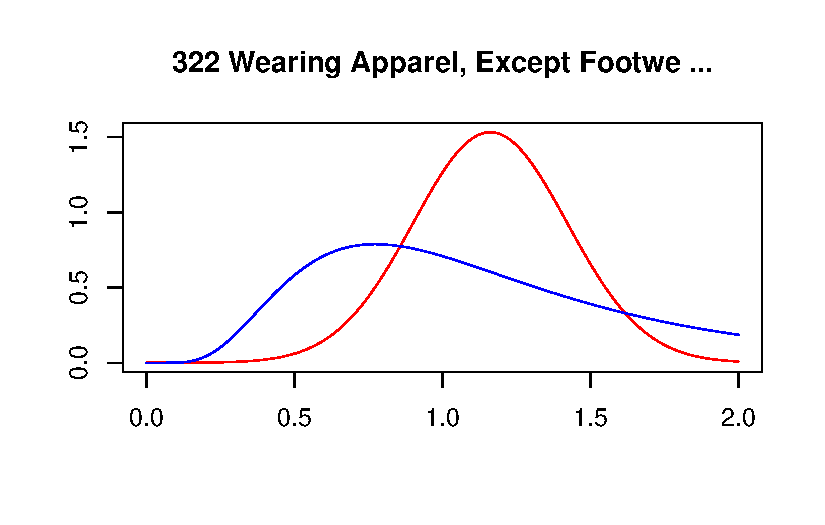
\includegraphics{Tax-Prod_files/figure-pdf/unnamed-chunk-35-1.pdf}

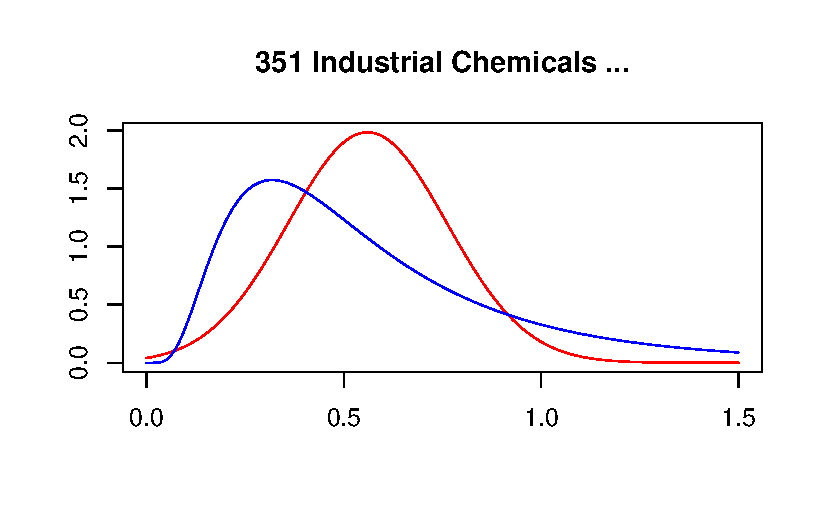
\includegraphics{Tax-Prod_files/figure-pdf/unnamed-chunk-35-2.pdf}

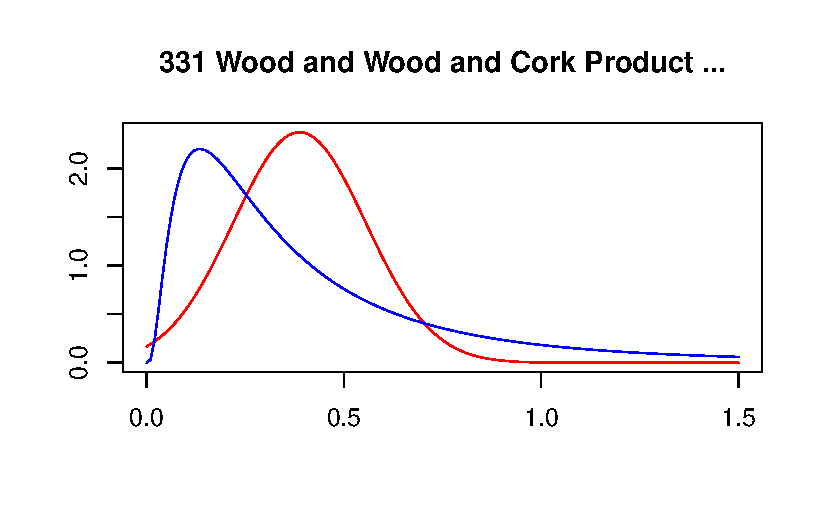
\includegraphics{Tax-Prod_files/figure-pdf/unnamed-chunk-35-3.pdf}

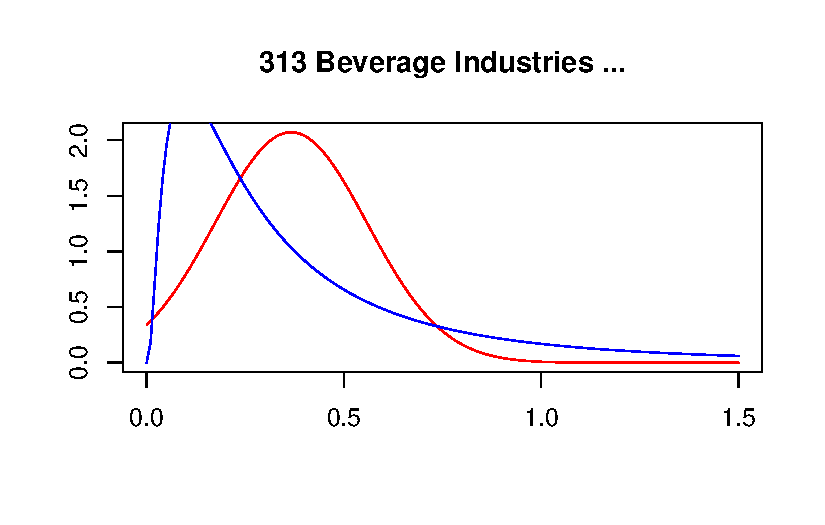
\includegraphics{Tax-Prod_files/figure-pdf/unnamed-chunk-35-4.pdf}

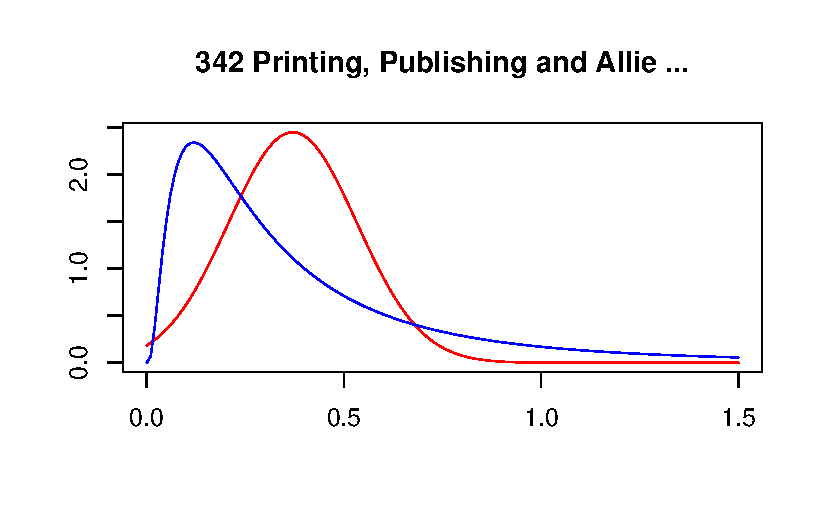
\includegraphics{Tax-Prod_files/figure-pdf/unnamed-chunk-35-5.pdf}

\begin{verbatim}
NULL
NULL
NULL
NULL
NULL
\end{verbatim}

\end{minipage}%

\caption{\label{fig-density-plots}Truncated Normal (red) and Log-Normal
(blue) distribution of the overreporting of raw materials for the top
tax-evading industries.}

\end{figure}%

\subsection{Production Function}\label{production-function}

\begin{table}

\caption{\label{tbl-CD-comparision}Cobb-Douglas production function
parameters estimates, correcting intermediates ---raw materials--- for
tax evasion vs.~naive estimation and OLS. \(h\) is a third degree
polynomial. \(Z={k_{it},l_{it}}\).}

\centering{

\centering
\begin{tabular}[t]{l|r|r|r|r|r|r|r|r|r}
\hline
\multicolumn{1}{c|}{ } & \multicolumn{3}{c|}{Tax Evasion + GNR} & \multicolumn{3}{c|}{GNR} & \multicolumn{3}{c}{OLS} \\
\cline{2-4} \cline{5-7} \cline{8-10}
  & m & k & l & m & k & l & m & k & l\\
\hline
322 & 0.0001 & 0.2464 & 0.6454 & 0.0014 & 0.4090 & 0.4365 & 0.3210 & 0.0693 & 0.6619\\
\hline
342 & 0.0092 & 0.3301 & 0.7470 & 0.3223 & 0.2486 & 0.4721 & 0.5210 & 0.0937 & 0.4569\\
\hline
313 & 0.3054 & 0.5384 & 0.4599 & 0.3316 & 0.3103 & 0.3427 & 0.7505 & 0.1156 & 0.2709\\
\hline
351 & 0.0539 & 0.5632 & 0.5483 & 0.2393 & 0.0169 & 0.2867 & 0.4794 & 0.3105 & 0.2461\\
\hline
331 & 0.3191 & 0.1601 & 0.8776 & 0.1233 & 0.1084 & 0.7333 & 0.4717 & 0.0677 & 0.5209\\
\hline
\end{tabular}

}

\end{table}%

\subsection{By Year}\label{by-year}

\section{References}\label{references}

\renewcommand{\bibsection}{}
\bibliography{biblio/export.bib,biblio/export2.bib,biblio/export3.bib,biblio/export31072022.bib,biblio/b100422.bib,biblio/b270123.bib,biblio/b100424.bib}




\end{document}
